%%%%%%%%%%%%%%%%%%%%%%%%%%%%%%%%%%%%%%%%%%%%%%%%%%%%%%%
%
%                                                       Example IS Template
%
% \documentclass{woosterthesis} must be at the beginning of every IS. Options are the same as
% for the report class with some additional options, abstractonly, blacklinks, code, kaukecopyright, palatino, picins,
% maple, index, verbatim, dropcaps, euler, gauss, alltt,  woolshort, colophon, woosterchicago, and
% achemso. The kaukecopyright option will put the arch symbol with the word mark on the
% copyright page. The woosterthesis class is based on the report class. One thing to note is that
% the ``%'' symbol comments out all characters that follow it on the line.
%
%%%%%%%%%%%%%%%%%%%%%%%%%%%%%%%%%%%%%%%%%%%%%%%%%%%%%%%

%Checked on 9/4/21 and compiles with no fatal errors. Users must have the latest version of the TeXLive software and have installed all available packages from CTAN to ensure this thesis class compiles with no fatal errors

%%%%%%%%%%%%%%%%%%%%%%%%%%%%%%%%%%%%%%%%%%%%%%%%%%%%%%%
% use this declaration for a draft  version of your IS
\documentclass[10pt,palatino,code,picins,kaukecopyright,openright,woolshort,dropcaps,verbatim,index,euler]{woosterthesis}
%\documentclass[10pt,code,picins,kaukecopyright,openright,woolshort,dropcaps,verbatim,euler,index,colophon,blacklinks,twoside]{woosterthesis}
% note that you can specify the woosterchicago option to use Chicago citation style and achemso to use the American Chemical Society citation format
%
%%%%%%%%%%%%%%%%%%%%%%%%%%%%%%%%%%%%%%%%%%%%%%%%%%%%%%%
%
% use this declaration for the print version of your IS
%\documentclass[12pt,code,palatino,picins,blacklinks,kaukecopyright,openright,twoside]{woosterthesis} % probably what most students would use
%
%%%%%%%%%%%%%%%%%%%%%%%%%%%%%%%%%%%%%%%%%%%%%%%%%%%%%%%
%
% use this declaration for the PDF version of your IS
% \documentclass[12pt,code,palatino,picins,kaukecopyright,openright,twoside]{woosterthesis}
%
%%%%%%%%%%%%%%%%%%%%%%%%%%%%%%%%%%%%%%%%%%%%%%%%%%%%%%%

%%%%%%%%%%%%%%%%%%%%%%%%%%%%%%%%%%%%%%%%%%%%%%%%%%%%%%%
%
%                                                       Load Packages
%
%   To load packages in addition to the ones that are loaded by default, please place your
%   usepackage commands in the packages.tex file in the styles folder.
%
%%%%%%%%%%%%%%%%%%%%%%%%%%%%%%%%%%%%%%%%%%%%%%%%%%%%%%%

%%%%%%%%%%%%%%%%%%%%%%%%%%%%%%%%%%%%%%%%%%%%%%%%%%%%%%%%%%%%%%%%%%%%%%%%%%%%%%%%%%%%%%%%%%%%%%
%
%                                                       Packages
%
% Do not add any other packages without consulting with Dr. Breitenbucher as they may break the functionality of the class.
%
%%%%%%%%%%%%%%%%%%%%%%%%%%%%%%%%%%%%%%%%%%%%%%%%%%%%%%%%%%%%%%%%%%%%%%%%%%%%%%%%%%%%%%%%%%%%%%

\ifxetex%
	\defaultfontfeatures{Mapping=tex-text}%
		\setmainfont[Numbers=OldStyle,BoldFont={* Semibold}]{Adobe Garamond Pro}% select the body font other choices would be Baskerville, Optima Regular, Didot, Georgia, Cochin
                      \setmathrm{Adobe Garamond Pro}
                      \setmathfont[Digits,Latin]{Adobe Garamond Pro}
		\setsansfont[Scale=.87,Fractions=On,Numbers=Lining]{Myriad Pro}% select the sans serif font other choices would be Skia, Arial, Helvetica, Helvetica Neue
%		\setmonofont[Scale=.88,Fractions=On]{Prestige Elite Std Bold}% set the mono font other choices would be Courier, Monaco, American Typewriter
	           \setmonofont[Scale=.9]{Courier Std}%
%	    \setromanfont[Fractions=On,Numbers=OldStyle, BoldFont={Warnock Pro Semibold}]{Warnock Pro}%
%	    \setsansfont[Scale=.95,Fractions=On,Numbers=Lining]{Myriad Pro}%
%	    \setmonofont[Scale=.91,Fractions=On]{Courier Std Medium}%
%	    \setmonofont[Scale=.88,Fractions=On]{American Typewriter}%
%		\setmonofont[Scale=.94,Fractions=On]{Prestige Elite Std Bold}
%    		\setromanfont[Fractions=On,Numbers=OldStyle]{Minion Pro}
 %    	\setsansfont[Scale=.9,Fractions=On,Numbers=Lining]{Myriad Pro}
%     	\setmonofont[Scale=.93,Fractions=On]{Courier Std Medium}
%     	\setromanfont[Fractions=On,Numbers=OldStyle]{Minion Pro}
%     	\setsansfont[Scale=.85,Fractions=On,Numbers=Lining]{News Gothic Std}
%    		\setmonofont[Scale=.93,Fractions=On]{Prestige Elite Std}
%		\setromanfont[Fractions=On,Numbers=OldStyle]{Minion Pro}
%		\setsansfont[Scale=.9,Fractions=On,Numbers=Lining]{Bell Gothic Std Bold}
%		\setmonofont[Scale=.95,Fractions=On]{Prestige Elite Std Bold}
\fi
\usepackage{dirtytalk}
\usepackage{color}
\usepackage{xcolor}
\usepackage{array}
\usepackage{listings}
\usepackage{musicography}
\usepackage{listing}
\lstset{
	language=c,
	basicstyle=\ttfamily\small,
	numberstyle=\tiny\color{gray},
	commentstyle=\color{teal},
	stringstyle=\ttfamily, % typewriter type for strings
	showstringspaces=false,
	keywordstyle=\color{blue},
	breaklines=true,
	postbreak=\mbox{\textcolor{red}{$\hookrightarrow$}\space},
	morekeywords={var, play, SynthDef, SinOsc, Sine, Saw, add, arg, EZSlider, EZKnob, controlSpec, initVal, action, label, labelHeight, labelWidth, Button, states_, Synth, MIDIClient, MIDIIn, action_, PinkNoise, Env, attackTime, decayTime, sustainLevel, releaseTime, peakLevel, curve, bias},
	frame=single,
	backgroundcolor=\color{white},
  	numbers=left,
  	stepnumber=1,    
  	firstnumber=1,
  	numberfirstline=true,
  	tabsize=1
}

%%%%%%%%%%%%%%%%%%%%%%%%%%%%%%%%%%%%%%%%%%%%%%%%%%%%%%%
%
%                                                       Load Personal commands
%                                                                    
%  There will be certain commands that you use frequently in the thesis. You can give these
%  commands new names which are easier for you to remember. You can also combine several
%  commands into a new command of your own. See The LaTeX Companion or Guide to LaTeX
%  for examples on defining your own commands. These are commands that I defined to cut
%  down on typing. You can enter your commands in the personal.tex file in the styles folder.
%
%%%%%%%%%%%%%%%%%%%%%%%%%%%%%%%%%%%%%%%%%%%%%%%%%%%%%%%

%%%%%%%%%%%%%%%%%%%%%%%%%%%%%%%%%%%%%%%%%%%%%%%%%%%%%%%%%%%%%%%%%%%%%%%%%%%%%%%%%%%%%%%%%%%%%%
%
%                                                       Personal Commands
%                                                                    
% There will be certain commands that you use frequently in the thesis. You can give these
% commands new names which are easier for you to remember. You can also combine several
% commands into a new command of your own. See The LaTeX Companion or Guide to LaTeX for
% examples on defining your own commands. These are commands that I defined to cut down on typing.
%
%%%%%%%%%%%%%%%%%%%%%%%%%%%%%%%%%%%%%%%%%%%%%%%%%%%%%%%%%%%%%%%%%%%%%%%%%%%%%%%%%%%%%%%%%%%%%%

% \newcommand{\fl}{\ell}
\newcommand{\lt}{\LaTeX\ }
\newcommand{\msw}{Word\texttrademark\ }
\newcommand{\xt}{\ifthenelse{\boolean{xetex}}{\XeTeX\ }{XeTeX} }
%\newcommand{\Cl}{\ensuremath{\textup{C}_\fl}}
%\newcommand{\bCl}{C$_{\ell}$}
%\newcommand{\Al}{\ensuremath{\textup{A}_\fl}}
%\newcommand{\msum}{{(m_1+\cdots+m_\ell)}}
%\newcommand{\Nsum}{{(N_1+\cdots+N_\ell)}}
%\newcommand{\ysum}{{(y_1+\cdots+y_\ell)}}
%\newcommand{\Nsub}{{N_1+\cdots+N_\ell}}
%\newcommand{\ysub}{{y_1+\cdots+y_\ell}}
%\newcommand{\xsub}{{x_1+\cdots+x_\ell}}
%\newcommand{\ysqsum}{{y_1^2+\cdots +y_{\fl}^2}}
%\newcommand{\msqsum}{{m_1^2+\cdots +m_{\fl}^2}}
%\newcommand{\ratio}{\left(\frac{\beta}{\alpha}\right)}
%\newcommand{\LT}{\ensuremath{\LaTeX{}}}

%%%%%%%%%%%%%%%%%%%%%%%%%%%%%%%%%%%%%%%%%%%%%%%%%%%%%%%%%%%%%%%%%%%%%%%%%%%%%%%%%%%%%%%%%%%%%%
% These commands have one argument and are entered as \commandname{argument}.
%%%%%%%%%%%%%%%%%%%%%%%%%%%%%%%%%%%%%%%%%%%%%%%%%%%%%%%%%%%%%%%%%%%%%%%%%%%%%%%%%%%%%%%%%%%%%%

%\newcommand{\bd}[1]{\textbf{#1}}
\newcommand{\mbd}[1]{{\mathbf{#1}}}
%\newcommand{\abs}[1]{\vert{#1}\vert}
\newcommand{\bvec}[1]{{\mbd{#1}}}
%\newcommand{\lvec}[1]{\abs{\bvec{#1}}}
%\newcommand{\nesmallprod}[1]{\prod_{\substack{#1=1\\
%#1\neq p}}^{\fl}}
%\newcommand{\esec}[1]{e_{2}({#1}_1,\ldots ,{#1}_\fl)}
%\newcommand{\smallprod}[1]{\prod_{#1=1}^{\fl}}
%\newcommand{\incsum}[1]{{#1}_2+2{#1}_3+\cdots +(\fl -1){#1}_\fl}
%\newcommand{\binomsum}[1]{\binom{{#1}_1}{2}+\cdots +\binom{{#1}_\fl}{2}}
%\newcommand{\imultsum}[1]{\multsum{{#1}_k\ge 0}{k=1,\ldots ,\fl}}
%\newcommand{\diagsum}[1]{\sum _{\substack{{#1}_k\ge 0\\
%k=1, \ldots ,\fl\\
%\lvec{#1}=m}}}
%\newcommand{\Mb}[1][\fl]{\ensuremath{\textup{\bd{M}}_b^{(#1)}}}
%\newcommand{\HLV}[1]{\ensuremath{\textup{\bd{H}}_{#1}}}
%\newcommand{\Rq}[1][p]{\ensuremath{\textup{R}_q^{(#1)}}}
\newcommand{\degree}[1]{\ensuremath{#1^{\circ}}}
\newcommand{\ip}[1]{\texttt{#1}\index{packages!#1}}
\newcommand{\ic}[1]{\texttt{$\backslash$#1}\index{commands!#1}}
\newcommand{\ie}[1]{#1\index{#1}}

%%%%%%%%%%%%%%%%%%%%%%%%%%%%%%%%%%%%%%%%%%%%%%%%%%%%%%%%%%%%%%%%%%%%%%%%%%%%%%%%%%%%%%%%%%%%%%
% These commands have 2 or more arguments some with default values for the first argument. You
% can learn a lot about constructing complicated equations by studying the commands in this %section.
%%%%%%%%%%%%%%%%%%%%%%%%%%%%%%%%%%%%%%%%%%%%%%%%%%%%%%%%%%%%%%%%%%%%%%%%%%%%%%%%%%%%%%%%%%%%%%

%\newcommand{\qbinom}[2]{\ensuremath{\left[{#1}\atop{#2}\right]_q}}
%\newcommand{\sqprod}[2]{\prod_{#1,#2=1}^{\fl}}
%\newcommand{\triprod}[2]{\prod_{1\le #1<#2\le \fl}}
%\newcommand{\nesqprod}[2]{\prod_{\substack{#1,#2=1\\
%#1,#2\neq p}}^{\fl}}
%\newcommand{\netriprod}[2]{\prod_{\substack{1\le #1<#2\le \fl\\
%#1,#2\neq p}}}
\newcommand{\qrfac}[3][\ ]{\left({#2}\right)_{#3}^{#1}}
%\newcommand{\multsum}[2]{\sum_{\substack{{#1}\\
%\\
%{#2}}}}
%\newcommand{\fmultsum}[2][N]{\multsum{0\le {{#2}_k}\le {{#1}_k}}{k=1,\ldots ,\fl}}
%\newcommand{\pq}[2]{\ _{#1}\varphi_{#2}}
%\newcommand{\mess}[2][y_k]{\frac{\qrfac{\alpha x_k}{#2}\qrfac{qx_k\beta^{-1}}{#2}}{\qrfac{\beta x_k}{#1}
%\qrfac{qx_k\alpha^{-1}}{#1}}}
%\newcommand{\MG}[7][\fl]{\ensuremath{\left[\textup{MG}\right]_{#2}^{(#1)}{#3}q;{#4};{#5}^{#6}{#7}}}

%%%%%%%%%%%%%%%%%%%%%%%%%%%%%%%%%%%%%%%%%%%%%%%%%%%%%%%%%%%%%%%%%%%%%%%%%%%%%%%%%%%%%%%%%%%%%%
% These commands define new environments
%%%%%%%%%%%%%%%%%%%%%%%%%%%%%%%%%%%%%%%%%%%%%%%%%%%%%%%%%%%%%%%%%%%%%%%%%%%%%%%%%%%%%%%%%%%%%%

\newcounter{unnumft}
\setcounter{unnumft}{0}
\newenvironment{unnumft}[2]{\renewcommand{\thefootnote}{}\footnote{#1}\footnote{#2}} {\addtocounter{footnote}{-2}}
\newenvironment{wooexample}{\small
\begin{singlespace}
\begin{example}}{\end{example}
\end{singlespace}}

\graphicspath{{./figures/}}% for setting where to look for figures
\citestyle{wooster}% change the style of citations. Math and CS people should leave this alone.






%%%%%%%%%%%%%%%%%%%%%%%%%%%%%%%%%%%%%%%%%%%%%%%%%%%%%%%
%
%                                                       Load Theorem formatting information
%
%  If you need to define an new theorem style or want to see what theorem like environments 
%  are available please look at the theorems.tex file in the styles folder.
%
%%%%%%%%%%%%%%%%%%%%%%%%%%%%%%%%%%%%%%%%%%%%%%%%%%%%%%%

\input{styles/theorems}

\setcounter{secnumdepth}{5}% controls the numbering of sections
\setcounter{tocdepth}{6}% controls the number of levels in the Contents

%%%%%%%%%%%%%%%%%%%%%%%%%%%%%%%%%%%%%%%%%%%%%%%%%%%%%%%
%
%  This is where one enters the information about the thesis.
%
%%%%%%%%%%%%%%%%%%%%%%%%%%%%%%%%%%%%%%%%%%%%%%%%%%%%%%%


\title{Developing a Virtual Modular Synthesizer for Sound Waves and MIDI}
\thesistype{Independent Study Thesis} % you should make this Independent Study Thesis
\author{Margaret Jagger}
% \presentdegrees{Ph.D.} % you should comment this line
\degreetoobtain{Bachelor of Arts in Computer Science}
\presentschool{The College of Wooster}
\academicprogram{Department of Mathematical \& Computational Sciences}
\gradyear{2022}
\advisor{Drew Guarnera (Mathematical \& Computational Sciences)}
%\secondadvisor{Second Advisor}
%\reader{Reader}
\copyrighted   
%\copyrightdate{}                  
\makeindex % comment this line if you do not have an index

%%%%%%%%%%%%%%%%%%%%%%%%%%%%%%%%%%%%%%%%%%%%%%%%%%%%%%%
%
%  This is where the commands for the document begin. All \LaTeX{} documents must have a
%  \begin{document} text .... \end{document} structure.
%
%%%%%%%%%%%%%%%%%%%%%%%%%%%%%%%%%%%%%%%%%%%%%%%%%%%%%%%

\begin{document}

%%%%%%%%%%%%%%%%%%%%%%%%%%%%%%%%%%%%%%%%%%%%%%%%%%%%%%%
%
%  The front matter includes acknowledgments, dedications, vitas, list of tables, list of figures,
%  copyright, abstract, title page, and contents.
%
%%%%%%%%%%%%%%%%%%%%%%%%%%%%%%%%%%%%%%%%%%%%%%%%%%%%%%%

\frontmatter
\maketitle
% \ClearShipoutPicture
\clearpage\thispagestyle{empty}\null\clearpage
\disscopyright 

%%%%%%%%%%%%%%%%%%%%%%%%%%%%%%%%%%%%%%%%%%%%%%%%%%%%%%%
%                                                                                       
%                                                       Abstract						
%                                                                                       
%%%%%%%%%%%%%%%%%%%%%%%%%%%%%%%%%%%%%%%%%%%%%%%%%%%%%%%

\begin{abstract}
Modular synthesis involves the alteration and modification of digital sound signals. Thus, this modular synthesizer allows a user the option of supplying their own MIDI-compatible controller to serve as an input source, or to use the built-in pure sound waves instead. Either input will be fed into the domain-specific language \textit{SuperCollider} and altered, with specific sound modifications dependent on the input source used. Using theoretical knowledge of the physics behind the motion of sound waves, various \textit{modules} and functionalities are created. Then, with \textit{SuperCollider}, these modules are implemented into a synthesizer which accepts either pure sound waves or MIDI as inputs, in a clean and easy-to-use interface. This modular synthesizer also has the potential to be continually expanded and improved upon beyond this initial version, with the option of adding other functionalities and sound modification options to augment the features currently available.
\end{abstract}

%%%%%%%%%%%%%%%%%%%%%%%%%%%%%%%%%%%%%%%%%%%%%%%%%%%%%%%
%                                                                                       
%                                                       Dedications					
%                                                                                       
%%%%%%%%%%%%%%%%%%%%%%%%%%%%%%%%%%%%%%%%%%%%%%%%%%%%%%%

% \dedication{This work is dedicated to the future generations of Wooster students.}


%%%%%%%%%%%%%%%%%%%%%%%%%%%%%%%%%%%%%%%%%%%%%%%%%%%%%%%
%                                                                                       
%                                                       Acknowledgments					
%                                                                                       
%%%%%%%%%%%%%%%%%%%%%%%%%%%%%%%%%%%%%%%%%%%%%%%%%%%%%%%

\begin{acknowl}  
I would like to acknowledge Prof. Lowell Boone in the Physics Department for his suggestions and code.
\end{acknowl}

%%%%%%%%%%%%%%%%%%%%%%%%%%%%%%%%%%%%%%%%%%%%%%%%%%%%%%%
%                                                                                       
%                                                       Vita					
%                                                                                       
%%%%%%%%%%%%%%%%%%%%%%%%%%%%%%%%%%%%%%%%%%%%%%%%%%%%%%%

%\begin{vita} 
% You talk about yourself and how you got to where you are now. There is a structured form for the Vita that can be used if you want, but I don't encourage it.

%%%%%%%%%%%%%%%%%%%%%%%%%%%%%%%%%%%%%%%%%%%%%%%%%%%%%%%
%
%  The list below is for a thesis that requires a more structured Vita such as a masters or Ph.D.
%
%%%%%%%%%%%%%%%%%%%%%%%%%%%%%%%%%%%%%%%%%%%%%%%%%%%%%%%

%\begin{datelist}
%\item[April 6, 1970]Born-Wooster, Ohio
%\item[August 11, 1990]Chosen to present an undergraduate paper at the 75th meeting of the MAA, Columbus, Ohio
%\item[August 1990--August 1991]President Wooster Student Chapter of the MAA, The College of Wooster, Wooster, Ohio
%\item[August 1991--May 1992]Secretary Wooster Student Chapter of the MAA, The College of Wooster, Wooster, Ohio
%\item[1992]\emph{Phi Beta Kappa} (on junior standing), The College of Wooster, Wooster, Ohio
%\item[1992]Elizabeth Sidwell Wagner Prize in Mathematics, The College of Wooster
%\item[1992]William H. Wilson Prize in Mathematics, The College of Wooster
%\item[May 11, 1992]B.A., Mathematics, The College of Wooster
%\item[1997]Finalist for Graduate Teaching Award, The Ohio State University, Columbus, Ohio
%\item[June 21-25, 1998]Participant in the AMS-IMS-SIAM Summer Research Conferences: q-Series, Combinatorics, and Computer Algebra, Mt. Holyoke, Massachusetts
%\item[October 1998--October 1999]Graduate student representative to The Ohio State University Department of Mathematics Graduate Studies Committee, Columbus, Ohio
%\item[January 1999]q-series seminar address, The Ohio State University, Columbus, Ohio
%\item[2000]Finalist for Departmental Teaching Award, The Ohio State University, Columbus, Ohio
%\item[2000]Nominated for Graduate Teaching Award, The Ohio State University, Columbus, Ohio
%\item[April 2000]Invited colloquium talk at The College of Wooster, Wooster, Ohio
%\item[1992-- present]Graduate Teaching and Research Associate, The Ohio State University
%\end{datelist}
%
%%%This is for any publications you might have.%%%%%

%\begin{publist}  
%\pubitem{\quad}
%\pubitem{\quad}
%\end{publist} 
%
%\begin{fieldsstudy} 
%    \majorfield{Major}
%	\minorfield{Minor}
%    \specialization{Area of IS research}
%    %\begin{studieslist}
%   %\studyitem{Abstract Algebra}{Hampton}
%   %\end{studieslist}
%  \end{fieldsstudy}
%\end{vita}

%%%%%%%%%%%%%%%%%%%%%%%%%%%%%%%%%%%%%%%%%%%%%%%%%%%%%%%
%
%  We now create the contents page and if necessary the list of figures and list of tables.
%
%%%%%%%%%%%%%%%%%%%%%%%%%%%%%%%%%%%%%%%%%%%%%%%%%%%%%%%


\cleardoublepage
\phantomsection
\addcontentsline{toc}{chapter}{Contents}

\tableofcontents
\listoffigures %Use if you have a list of figures.
\listoftables%Use if you have a list of tables.
\lstlistoflistings% Use if you are using the code option

%%%%%%%%%%%%%%%%%%%%%%%%%%%%%%%%%%%%%%%%%%%%%%%%%%%%%%%

%\input{chapters/preface} % most theses do not have a preface so this should be commented

%%%%%%%%%%%%%%%%%%%%%%%%%%%%%%%%%%%%%%%%%%%%%%%%%%%%%%%
\mainmatter

%%%%%%%%%%%%%%%%%%%%%%%%%%%%%%%%%%%%%%%%%%%%%%%%%%%%%%%
%
%                                                       Thesis Chapters
%
% This is where the main text of the thesis goes. I have written this template assuming that
% each chapter is a separate file. You do not have to do this but it makes things easier to find
% for editing. You can use the sample chapters to help you figure out how to type things into
% your thesis. To include a chapter just use the \include{chaptername} command. Chapters are
% included in the order listed.
%
%%%%%%%%%%%%%%%%%%%%%%%%%%%%%%%%%%%%%%%%%%%%%%%%%%%%%%%

%!TEX root = ../username.tex
\chapter{Introduction}\label{chapter:intro}

Within the world of digital signal processing (DSP), digital audio, and physical instruments, there are almost limitless possibilities available now to create sounds through computers, whether through synthesis, production, or mixing. Ultimately, the products which result from explorations between computer science and music are dependent on the creator's familiarity with both fields. Current applications for music synthesis are sufficient in usability, with Helm, an open-source modular synthesizer, as one example. One is easily able to find Helm through an Internet search, download the application, and begin altering an input's sound to their liking, provided they have a MIDI controller on hand to serve as the input device. Thus, the primary goal of this thesis is to create a modular synthesizer with two options for inputs: MIDI and pure sound waveforms, such as sine waves. 

There are three goals that must be accomplished in order to provide a modular synthesizer which utilizes both MIDI and pure sound waveforms: synthesizing (creating) pure sound waveforms through our language of choice \textit{SuperCollider}, accepting MIDI as an input option, and altering either input properly so the sound modification is obvious. So, this project relies on knowledge of both digital signals (the detectable digital impulses through which messages or other information can be transmitted \cite{Rosen_Howell_2011}), for MIDI input, as well as waveforms types, and mathematically, the ways in which we are able to alter these signals. Creating a virtual modular synthesizer requires a significant amount of programming in the domain-specific language SuperCollider, which connects the input from a physical MIDI controller and pure sound waveforms to the desired sound modifications. Thus, there will be a front-end graphical user interface, as well as a back-end which is connected to the signal modification modules. The front-end will provide users with a way to easily interpret and understand the modules of this synthesizer, and the back-end will process the desired sound changes the user has input, and output these alterations. The back-end includes modules typically found in open-source and commercial modular synthesizers, including, but not limited to: volume control, pitch bend, harmonics layering, delay, legato and staccato, distortion, and manual MIDI adjustments. This virtual modular synthesizer successfully completes each of these goals, and will serve as the primary product of this thesis.

Several of these modules, or functionalities which are able to act independently from each other, are self-explanatory; the pitch bend will alter the perceived pitch (frequency) of the input note, and the volume control will adjust the sound's loudness. The other modules mentioned are less intuitive. Harmonics layering involves layering various frequencies, whether the same or slightly different, over one another. Delay affects how early or late a note is perceived to be played. Legato, as defined in music, is the playback of notes in a connected manner, and staccato is the opposite, the playback of notes in a detached and separated way. Distortion typically is a \textit{destructive} effect, in which the sound to be distorted cannot be reverted back to its previous state. For this modular synthesizer, distortion will act as another version of harmonics layering, adding unneeded and unpleasant sounds to a user's input. For MIDI input, there is also an option to manually adjust the sound output a user receives, through adjusting an \textit{ADSR envelope}, or the Attack, Decay, Sustain, and Release of a MIDI note.

First, we will provide an introduction to the field of DSP, sound synthesis, and MIDI, and SuperCollider, the domain-specific programming language used for this project. This discussion will include context on previous developments on modular synthesizers and define the difference between modular sound synthesis and other types of synthesis. The modular synthesizer, specifically, is a type of synthesizer, or electronic instrument, which is able to produce a wide variety of sounds, through sound modifications, in a single unit with a unified control system. Then, we discuss the important mathematical details which are relevant to the creation of this modular synthesizer. Specifically, this will include the various types of waveforms, and the ways in which the waves can be manipulated. After, we go into detail of the process of developing the modular synthesizer, and the step-by-step description of the ways in which each module was developed. Some modules proved to be more challenging to implement than others, and so we also provide context as to how a particular module is developed. Finally, we finish with a conclusion discussing the challenges of implementing this synthesizer, the ways in which this synthesizer could be expanded or improved, and suggestions for future work.
%!TEX root = ../username.tex
\chapter{Background}\label{chapter:background}
% terms mentioned often
% sine wave

\section[History of Modular Synthesizers]{History of Modular Synthesizers}\label{section:mod-synth-history}

The 1950s was a turning point within the field of electronic music and communicational technologies. This marked the creation of electronic music, with the use of physical componenets. Electronic music was rare, with synthesizers\footnote{As described in section \ref{modular-synth-what-is}.} and electronic instruments\footnote{Examples of these would include electric guitars, electric keyboards, and more.} being less common. So also were modular synthesizers, at that point containing fewer modules\footnote{The concept of modules will be further discussed in section \ref{modular-synth-what-is}.} than found in modular synthesizers today. These modular synthesizers were large, taking up significant space, as evidenced by Bode's Audio System Synthesizer and Moog's Minimoog Model D, two influential analog modular synthesizers discussed later in this section.

The first module, or functionality, created was the positive feedback oscillator, sometime between 1912 and 1914 \cite{Gabrielli_2020}.\footnote{This module is now commonly found in modular synthesizers today, both analog (physical) and digital (virtual).} A positive feedback oscillator--or as it is known today, the simple oscillator--produces sounds within a synthesizer, specifically a repeated signal (the audio wave) which periodically rises and falls. This is where the oscillator module gets its name, producing a sound which rises and falls, or oscillates.\footnote{The method through which the oscillator creates the audio waveform affects the resulting waveform, of which examples are discussed in chapter \ref{theory}. For now, it is important to note that oscillators will produce one of four waveforms typically: sine waves, triangle waves, sawtooth waves, and square waves, or pulse waves.} The creation of this positive feedback module is attributed to Austrian engineer and physicist Alexander Meissner. Unlike the oscillator module found today, the early version was only able to last a few minutes. Instead of continuously able to produce an audio waveform, this version produced only a small output of power \cite{Fleming_1919}. 1912 introduced the communicational technologies field as something more than niche. Products from proper physics laboratories were rare to find, and so were machines capable of producing audio waveforms with high frequencies after several minutes. Meissner created a new type of machine through the use of feedback: a high-frequency generator from an amplifier, with a vacuum tube as a substitute for a high-frequency receiver machine \cite{Fleming_1919}. Previous to Meissner's creation, it was impossible to establish a connection between a high-frequency machine with a receiver. The output frequency of such a machine was not the same as the user's desired output frequency, a synchronous and superimposed frequency. Meissner's product was easier to handle than these machines, and much more useful. In addition, Meissner's machine was much less noisy as well. This machine could change the output frequency given to the receiver, and tune the receiver machine to a range of wavelengths that were previously not possible \cite{Fleming_1919}. This development changed the process of receiving wavelengths. The un-dampened wave\footnote{An un-dampened audio wave is a typical audio wave. The wave continues to oscillate without any force or opposing motion to stop it from oscillating. This differs from a dampened wave. A dampened wave is an audio wave which oscillates, yet there is some force or opposing motion which slows the wave down. Eventually, the wave will lose energy such that it stops oscillating, unless there is a force or motion to keep the wave oscillating.} which resulted allowed for a user to fine-tune the frequency, while also suppressing any atmospheric distractions or sounds. With Meissner's work, the field's knowledge of constant sound generation and high frequencies was expanded, and paved the way for future work on the short-wave band \footnote{Though not discussed in this paper, the short-wave band is typically used in maritime communications, international, and radio broadcasting. More reading on Alexander Meissner and his patented solution can be found in the Engineer and Technology History Wiki's page on Alexander Meissner here: \url{https://ethw.org/Alexander_Meissner}}.

Then, sometime between 1959 and 1960, Harold Bode (1909-1987), a German engineer, created the modular synthesizer which we are familiar with today. Bode was a German engineer and designer of audio tools. He foresaw that transistor technology\footnote{A transistor is a semiconductor device which is used to amplify, control, and generate electrical signals. These are active components for integrated circuits, or \say{microchips}. Transistors are tiny, and so these microchips will often contain billions of transistors, etched into their surfaces. Today, transistors have become embedded into almost everything electronic.} would become a key change in creating and designing synthesizers, especially modular synthesizers\cite{Gabrielli_2020}. Transistors would link the audio signal through cables, through where each component, or \say{module} could be connected in any order, according to the user's preferences. Multiple modules--including modulators, filters, reverberation generators, and more--could then be connected in any order, either to modify or generate sounds. With transistor technology, Bode created his \textit{Audio System Synthesizer}, which allowed for a larger number of sound creation possibilities than before. The system itself contained inputs for various sound sources, and the input signals could be modified by filter modules and a modulator\cite{Bode_1984}. As the system was modular, there were independently working modules for sound modification. These modules could be combined with each other in several ways, according to the user's desired order. This Audio System Synthesizer also made an impression on Robert Moog, who would take Bode's idea and further develop it \cite{Gabrielli_2020}. 

Robert Moog (1934-2005) was an American engineer inspired by Harold Bode's Audio System Synthesizer. As the inventor of the first commercial synthesizer, dubbed the Moog synthesizer, Moog created the first integrated synthesizer. The Moog synthesizer was built in 1964, and contained several of the fundamental synthesizer concepts found today\cite{Pinch_Trocco_2004}. These modules on the Moog synthesizer included the voltage-controlled modules, envelope generators\footnote{Envelope generators will be dicussed in more depth in section \ref{modular-synth-what-is}}, and the pitch wheel. With the Moog synthesizer, synthesizers were brought to a wider audience, influencing the development of popular music\cite{Pinch_Trocco_2004}. What followed the Moog synthesizer was the Minimoog Model D, a portable 1970 creation. The Minimoog Model D is acknowledged to be the most \say{influence synthesizer of all time}\cite{Gabrielli_2020} due to its playability and compactness. Similar to the Moog synthesizer, it included modules to both generate and shape sounds \cite{Pinch_Trocco_2002}.

The 1960s also saw the introduction of Donald \say{Don} Buchla, and his Buchla 100 Series Modular Electric Music System. Don Buchla (1937-2016) was another American inventor, working in the field of sound synthesis independently of Robert Moog. The Buchla 100 Series (otherwise known as the \say{Buchla Series 100} or \say{Buchla Box}), is a keyboard-less modular synthesizer. Unlike Moog's Moog synthesizer and Minimoog Model D, the Buchla 100 Series used a more manual control\cite{Pinch_Trocco_1998}. Instead of a keyboard for user input, the user would control the synthesizer's modules directly. It contained a logical layout, with an intuitive, user-facing front panel, which allows the user to directly patch and route modules together, using patch cords. With the various knobs and triggers on the synthesizer itself, a user could manipulate sound according to multiple parameters. Along with user input differences, there were other important distinctions between the Buchla and Moog synthesizers. These changes include Buchla's use of voltage-controlled oscillators with multiple complex modulation options, and a decrease in emphasis on using filters. This methodology would lead to a division in school of thought: the East Coast school of thought, and the West Coast school of thought \cite{Gabrielli_2020}. The West Coast method, which was led by Buchla, put greater emphasis on the experimental side of electronic music, and so designed their synthesizers according to this.

Both the East Coast and West Coast methods of audio synthesis are important, as they eventually become the two general methods for synthesis: additive synthesis and subtractive synthesis\footnote{Additive synthesis and subtractive synthesis are two other types of audio synthesis.}. In a general overview, the East Coast approach embodies a straightforward and practical approach, with efficiency and reliability as important concepts. West Coat synthesis instead focuses on experimentation, with a non-traditional sound that is generated. For East Coast audio synthesis, its patches and way of forming modules fall under the category of \say{subtractive synthesis}. Subtractive synthesis involves starting with a complex audio waveform, with multiple harmonics (i.e. pitches, or notes)\cite{Winer_2018}. Then, a low-pass filter (or in analog synthesizers, a voltage-controlled low-pass filter, or VCF) slowly removes selected frequencies from the complex wave. The sound produced by West Coast synthesis is less known that East Coast synthesis. In place of aspiring towards a sense of musical efficiency, the West Coast method evolved out of the desire to replicate the acoustically-generated tones through manipulating previously recorded sounds\cite{Nielsen}. Thus, the West Coast method is not centered around a singular principle. It combines elements of additive synthesis\footnote{This is defined as the addition of multiple, simple audio waveforms together to create a complex, composite waveform. These are often sine waves.}\cite{Nielsen} and frequency modulation to create many sounds of complex timbres. Both additive and subtractive synthesis will be discussed further in the next section.

\section[Modular Synthesis: What Is It?]{Modular Synthesis: What Is It?}\label{modular-synth-what-is}

A modular synthesizer is a type of synthesize which is composed of separate modules for different functions. These modules, in a physical hardware synthesizer, would be connected together by the user to create a \say{patch}. The output from these modules would then be audio signals, voltages, or digital signals for various logical or timing conditions. Typically, these modules would include voltage-controlled oscillators, voltage-controlled filters, voltage-controlled amplifiers, and envelope generators.\footnote{The need for voltage-controlled modules was such that the modules would not receive sufficient power otherwise to properly function.} Within a virtual modular synthesizer, we have no need for these voltage-controlled modules. However, we still must \say{patch} these modules together in a linear sort of way, and decide the order in which the modules are applied to a digital signal. 
\section[MIDI: An Introduction]{MIDI}\label{section:midi}

\subsection[What is MIDI?]{What is MIDI?}\label{section:what-midi}
The Musical Instrument Digital Interface (more commonly known as MIDI) is a digital communications protocol which allows for multiple hardware and software electronic instruments, controllers, computers, and related devices to communicate over a connected network\cite{Huber_2012}. It is used most to translate performance \say{events} (or musical notes) into its equivalent digital message, and then transmit these messages to other MIDI devices. These devices (MIDI receivers) can control sound generators or performance generators to create or modify music. Any MIDI-compatible device can send or receive MIDI messages from a MIDI controller (or the device sending the MIDI messages), and this will include all types of synthesizers. As an \say{interface,} MIDI is composed of a data communications link, and a system of hardware and software connected through this MIDI network. With MIDI, any electronic instruments and devices which are within a network can be worked with, through the transmission of a real-time performance and MIDI messages. These transmissions of performances and messages can then be put through the system to various instruments and devices through one singular data line, rather than multiple data streams, as this system can be chained from one device to another. A single data cable used with MIDI is capable of transmitting a real-time performance and MIDI-control message over 16 distinct channels, numbered appropriately one through sixteen. The musician working with the system will determine which of these channels to send information through, depending on which MIDI devices are being used\cite{Romano_2003}.

However, there are several limitations to the MIDI protocol. The first, and most important, limitation of MIDI is that it does not support sound. It is unable to communicate audio itself, or create sounds\cite{Huber_2012}. Instead, as a digital language, it instructs a compatible device or program to create, playback, or modify sounds. It will communicate an on/off status of a sound trigger, along with a range of parameters which instructs a MIDI receiver to control specified audio-related functions \cite{Kirk_Hunt_2013}. So, the data pathways for MIDI and audio routing will be different, even if they share a physical transmission cable, as in Figure \ref{fig:midi-system-with-audio-connections}\cite{Huber_2012}. 

\begin{figure}
	\centering
	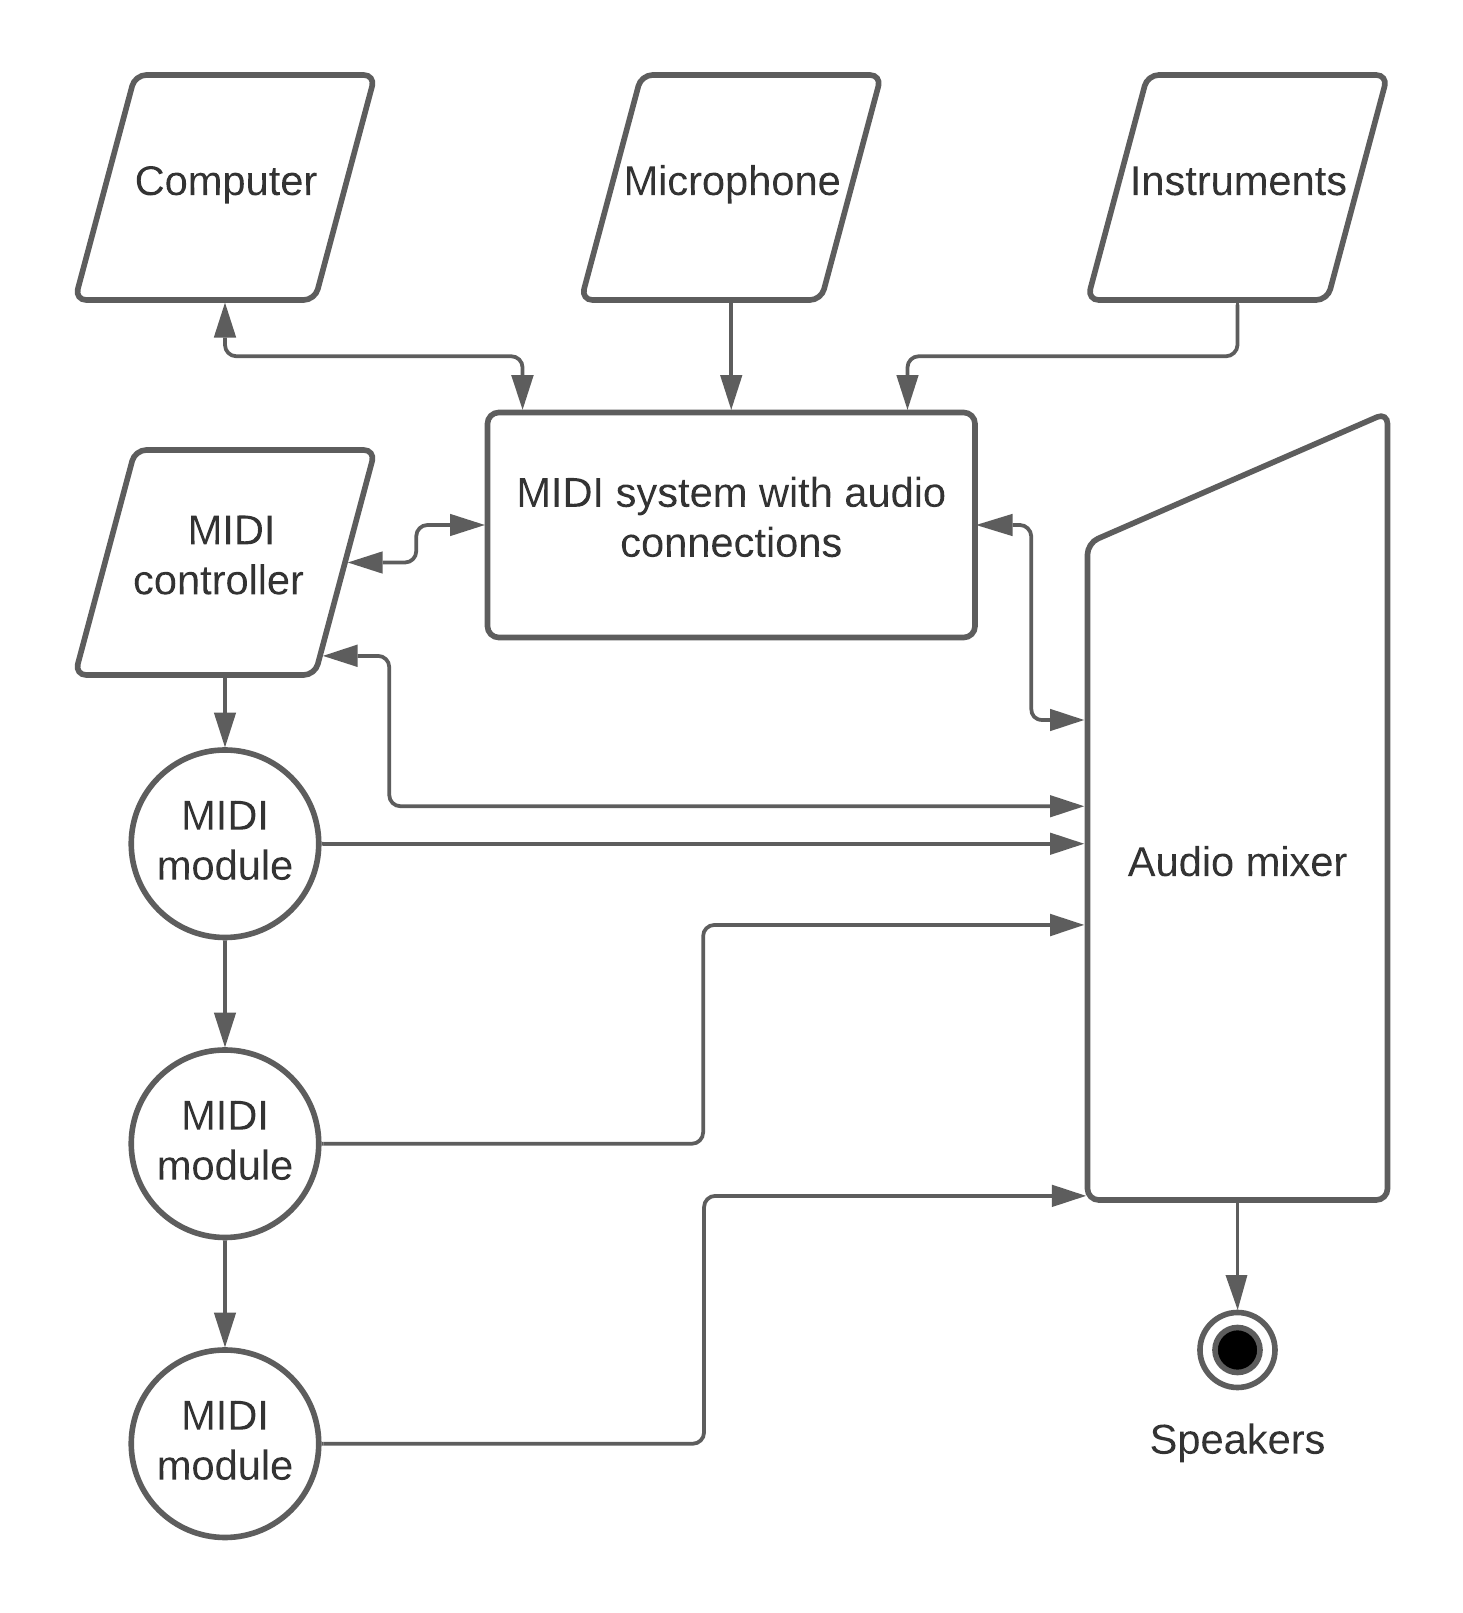
\includegraphics[width=0.35\textwidth]{figures/midi-system-with-audio-connections.png}
	\caption{The MIDI system, with audio connections}
	\label{fig:midi-system-with-audio-connections}
\end{figure}

Additionally, much of MIDI is built around the concept of keyboard notes and pitches. MIDI messages are primarily transmitted through the use of an electronic keyboard. So, for other types of MIDI instruments (such as a violin, or clarinet), there is a restriction to how a note may sound using MIDI. Certain characteristics of non-keyboard instruments (such as the ability of playing discrete semitone pitches) are more easily lost. For players of acoustic instruments, these issues are even more clear. Within MIDI, the velocity is considered to be a single note-on velocity, defining the dynamic response of the note to one value. For players of acoustic instruments, the velocity, or dynamic response, of a singular note is shaped by the player, along with the note's timbre and pitch when played\cite{Kirk_Hunt_2013}.

% TODO: explain discrete semitone pitches

\subsection[How does MIDI work?]{How does MIDI work?}\label{subsection:how-midi}
From a hardware perspective, the MIDI protocol will determine which types of plugs can be used for MIDI connections. There are three possible \say{sockets} that can be used on any MIDI-compatible device:

\begin{enumerate}
	\item MIDI OUT: this will send data to other devices (MIDI receivers). An example of this will include an electronic keyboard which plays a note, and then \say{note messages} are sent out from the MIDI OUT socket.
	\item MIDI IN: this socket will receive the MIDI information from other devices. Using the previous example, if a keyboard's MIDI OUT socket is connected with a MIDI cable to another sound module's IN socket, then the sound module will be able to produce sound on behalf of the keyboard.
	\item MIDI THRU: this socket will relay the messages received at the MIDI IN socket, so more devices will be able to be chained together.
\end{enumerate}\label{enu:list-of-midi-sockets}

\begin{figure}
	\centering
	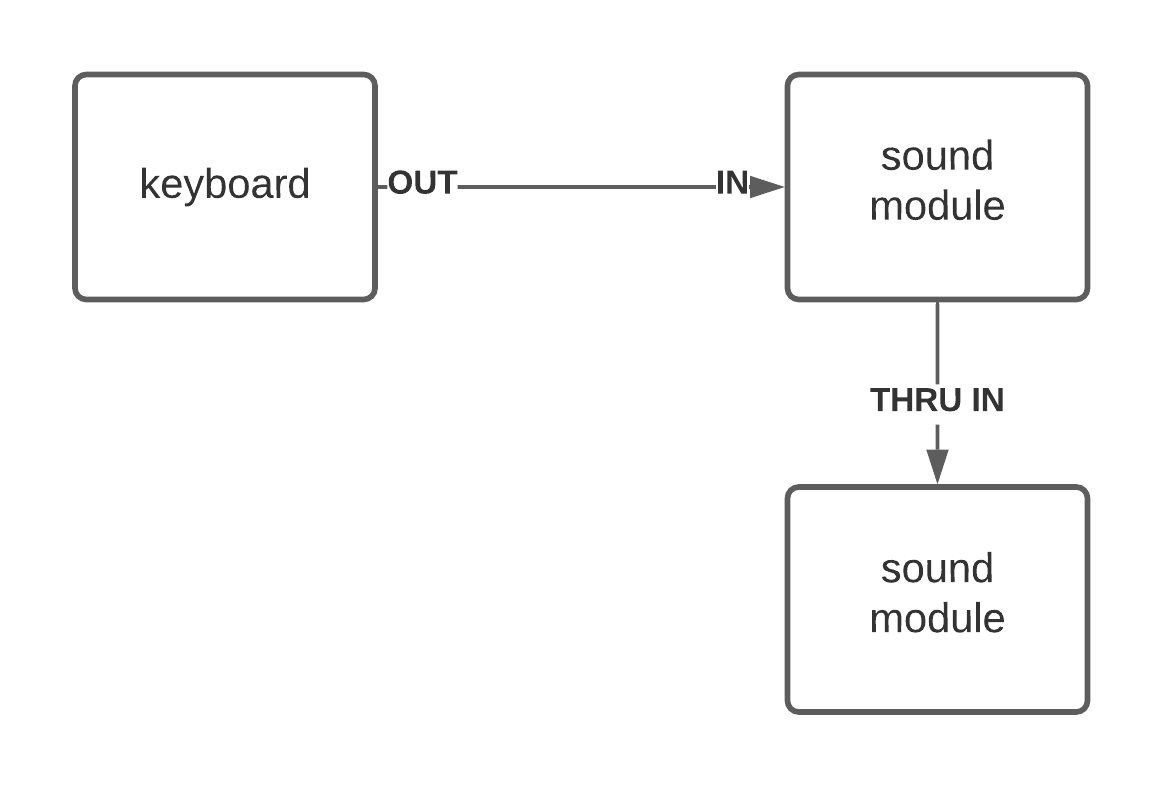
\includegraphics[width=0.5\textwidth]{figures/midi-sockets.png}
	\caption{MIDI sockets using an electronic keyboard}
	\label{fig:midi-sockets}
\end{figure}

Typically, this will result in the flow in Figure \ref{fig:midi-sockets}, as it is normal for a keyboard's OUT port to be connected to a sound module's IN port. This IN socket will then be connected to another sound module, through the THRU IN port of the first sound module, into the IN port of the second sound module. Thus, both modules are now driven by the keyboard\cite{Kirk_Hunt_2013}.

In a software view of the protocol, there are two basic types of messages MIDI is able to send: a \textit{channel} message, and a \textit{system} message. Channel messages are much more common. As previously mentioned, MIDI allows for the use of up to 16 different sounds to be controlled at the same time, through the use of its 16 different channels. So, each sound that must be played concurrently will be placed into a different \textit{MIDI channel}. Within the channel, there are seven distinct messages, each of which contain a specific meaning and role. The first is the \say{Note on} message. This is the most common MIDI message used, and is sent whenever a note on a MIDI controller is played or pressed down, most common as pressing a key on a keyboard. The data contained in this message will tell a sound module how hard and fast a note was played (the \textit{velocity} of a note), as well as which channel the note was played on\cite{Romano_2003}. The pitch of the message represents which key was pressed, and is defined as the number for each semitone on a keyboard. The semitone is the smallest interval of the modern Western tonal system. In equal temperament\footnote{Equal temperament is regarded to be the normal tuning of the West, a 12-note chromatic scale. This is also known as A440, in which the note $A_4$ is tuned relative to the standard pitch of 440Hz, and other notes are tuned as a specific number of semitones from this pitch.}--a tuning of the scale, based on a cycle of 12 identical fifths, and with the octave divided into 12 equal semitones--a semitone is the $\frac{1}{12}$ part of an octave. The notational system (i.e. sheet music) allows for three types of semitones to be distinguished: the diatonic, or the minor second (e.g. E-F, or C\musSharp{}-D), the chromatic, the difference between a major second and a minor second (e.g. F-F\musSharp{}, or D\musFlat{}-D), and the enharmonic, the doubly diminished third (e.g. G\musFlat{}\musFlat{}-E) \cite{Drabkin_Lindley_2001}. Middle C ($C_4$) is number 60 on the keyboard, and each semitone above and below Middle C is incremented or decremented accordingly\cite{Kirk_Hunt_2013}. 

The second is the \say{Note off} message, which turns off a note, or notes when a note is stopped. Like with Note on, Note off also contains values for channel, pitch, and velocity. For this message, only velocity's definition is changed, referring instead to the speed at which a note is released. The final common type of channel MIDI message is the \say{Pitch-bend,} which for electronic keyboard appears in the form of a physical wheel or sideways-moving handle of some type. Like its name implies, users will use this wheel or module to bend the pitch of notes currently being played. If the module is a physical wheel, it will return to its default position of zero (not bending a note) when the player lets go of the wheel. The pitch-bend will contain two pieces of data: the channel, and the pitch bend value. This value ranges from 0-127, with a value of 0 representing that the pitch has a full downwards bend to it, while a value of 127 represents the opposite, with a full upwards bend\cite{Kirk_Hunt_2013}. For this module, the value 64 will roughly indicate the center position on the wheel, and represent that a pitch has no bend applied to it.

MIDI also contains \say{system} messages, sent to all devices within the MIDI system\cite{Romano_2003}. These messages are not limited to a specified number of channels, and allow for a greater variety of data to be sent. There are three basic types of system messages\cite{Kirk_Hunt_2013}:

\begin{enumerate}
	\item real-time: this type of message allows the devices within the MIDI system to synchronize together.
	\item common: this message allows the devices to agree on some type of common musical issues, with tuning and song selection as two examples.
	\item exclusive: this message will exclusively send data to one device type. For manufacturers, these messages are used to send data to only one type of synthesizer or device type, serving as \say{add-ons} to MIDI.
\end{enumerate}\label{enu:midi-system-messages}

\noindent System messages are much harder to understand than channel messages, and so will not be discussed to great detail within the scope of this project.

\subsection[Constructing MIDI Messages]{Constructing MIDI Messages}\label{section:midi-messages}

MIDI messages are composed of three bytes, with a byte defined as a fundamental computation building block which consists of eight binary digits (or bits), either zero or one. Bytes which begin with a zero will be a \say{data byte} and bytes which begin with a one are \say{status bytes.} The most significant bit (MSB, or the leftmost binary bit within a MIDI message) is used to identity the byte type. The MSB of a data byte is 0, while the MSB of a status byte is 1.

\[\textrm{a status byte: } \textit{1xxx nnnn} \] \[\textrm{a data byte: } \textit{0nnn nnnn} \]

A status byte determines the type of MIDI function that will be performed, and encodes channel data, allowing the instruction to be received by a device that is set to respond to the selected channel. A data byte is used to associate a certain value to the event that is given by the accompanying status byte. This will determine the type of message that is sent (as they are normally channel messages) between note on, note off, pitch bend, or another type of message.

% TODO: this is confusing 
After the top bit/MSB of one in a status byte, which begins a MIDI message, the next three bits, or digits, are the bits which actively determine the type of message it is, of which there are eight possible combinations:

\[000, 001, 010, 100, 101, 110, 111 \]

The last four bits of a MIDI message determine which channel the message is delivered through, with 16 combinations for each of the 16 channels, as seen below. %TODO: fix the tables, so this makes sense

% TODO: have better transition between last section to talking about individual message types
\subsubsection{Note On Messages}

The note on message indicates the beginning of a MIDI note. Typically, one note on message is generated each time a note is triggered on a MIDI device, such as a keyboard, controller, or other MIDI instrument\footnote{This includes, pressing down a key, hitting a MIDI drum pad, or playing a MIDI sequence.}. A note on message will contain three bytes of information: the MIDI channel number, the pitch number, and the attack velocity value. As in Table \ref{tbl:byte-structure-note-on}, the first byte specifies that this MIDI message is a note on message, and the MIDI channel that this message will go through. The second byte determines the specific note, of the possible 128 notes numbered 0-127, which will be sounded by the MIDI instrument. The third and final byte of a note on message is the note's velocity, also ranged from 0-127. This will denote the loudness of the sounding note, increasing in volume the higher this value goes. For MIDI instruments which do no interpret the entire 128-numbered range of velocity values, we will instead see an attack velocity value of 64 used, regardless of how loud or soft the note itself may be played. This value of 64 gives the note a dynamic/loudness of \textit{mezzo forte}, or moderately loud. Additionally, a note on message with an attack velocity of 0 will generally be equivalent to a note off message, discussed in the next section. In a note on message with an attack velocity value of 0, the MIDI receiver will generally silence the currently-sounding note, by playing it with a velocity (or volume) value of 0\cite{Huber_2012}.

\begin{table}
	\centering
	\begin{tabular}{|c|c|c|}
	\hline
		Channel number (0-15) & Note number (0-127) & Attack velocity (0-127) \\
		\hline
		(1001 CCCC) & (0NNN NNNN) & (0VVV VVVV) \\
	\hline
	\end{tabular}
	\caption{The structure of a note on MIDI message}
	\label{tbl:byte-structure-note-on}
\end{table}

\subsubsection{Note Off Messages}

\begin{table}
	\centering
	\begin{tabular}{|c|c|c|}
	\hline
		Channel number (0-15) & Note number (0-127) & Release velocity (0-127) \\
		\hline
		(1001 CCCC) & (0NNN NNNN) & (0VVV VVVV) \\
	\hline
	\end{tabular}
	\caption{The structure of a note off MIDI message}
	\label{tbl:byte-structure-note-off}
\end{table}

A note off message is similar to that of a note on message, except that it is a command used to stop playing a MIDI note. A MIDI note on message will play until a corresponding note off message for that note is received by the MIDI receiver. So, a musical composition can, in its most basic form, be written as various MIDI note on and note off messages. There are also three bytes in a MIDI note off message (refer to table \ref{Tbl:byte-structure-note-off}), except that the third byte instead is a release velocity value. This value, also ranging from 0-127, will indicate the velocity in which a key or controller is released. A lower value indicates that the key was released slowly, and a higher value shows the key was released quickly. For MIDI devices which are able to respond to receiving a release velocity value, these are able to be programmed to vary the note's speed of decay, reducing the note's decay time as the release velocity value increases\cite{Kirk_Hunt_2013}. %TODO: explain what MIDI decay is

\subsubsection{Pressure/Aftertouch Messages}

\begin{table}
	\centering
	\begin{tabular}{|c|c|c|}
	\hline
		Channel number (0-15) & Note number (0-127) & Release velocity (0-127) \\
		\hline
		(1000 CCCC) & (0NNN NNNN) & (0VVV VVVV) \\
	\hline
	\end{tabular}
	\caption{The structure of an aftertouch MIDI message}
	\label{tbl:byte-structure-aftertouch}
\end{table}

Pressure messages, also known as \say{Aftertouch} messages, happen after a key is pressed, and the user decides to press down on the key harder. For compatible MIDI devices, aftertouch can generally be assigned to parameters which include vibrato, volume, filter cutoff, and pitch. As defined by MIDI, and the byte structure of an aftertouch message in Table \ref{tbl:byte-structure-aftertouch}, there are two types of aftertouch messages: channel pressure messages and polyphonic key pressure messages\cite{Huber_2012}. %TODO: define all the music terms

\begin{table}
	\centering
	\begin{tabular}{|c|c|c|}
	\hline
		Channel number (0-15) & Note number (0-127) & Pressure value (0-127) \\
		\hline
		(1101 CCCC) & (0NNN NNNN) & (0VVV VVVV) \\
	\hline
	\end{tabular}
	\caption{The structure of a channel pressure MIDI message}
	\label{tbl:byte-structure-channel-pressure-messages}
\end{table}

Channel pressure messages are messages commonly transmitted by instruments which only respond to a singular overall pressure, regardless of the total number of keys played. These messages also contain three bytes of information: the MIDI channel number, the note number, and pressure value, as in table \ref{Tbl:byte-structure-channel-pressure-messages}\cite{Huber_2012}. 

Polyphonic key pressure messages are similar to channel pressure messages, but respond to the pressure changes that are applied to the individual keys of a MIDI keyboard. A MIDI device compatible with this type of MIDI message is able to respond or transmit the individual key pressure messages of each key that is pressed down. How a MIDI device compatible with polyphonic key pressure messages will vary, but typically contain bindings for performance parameters which include vibrato, volume, timbre, and pitch\cite{McGuire_2014}. %TODO: this last sentence doesn't make 100% sense, make better -> define timbre

\subsubsection{Program Change Messages}

\begin{table}
	\centering
	\begin{tabular}{|c|c|}
	\hline
		Channel number (0-15) & Program ID number (0-127) \\
		\hline
		(1100 CCCC) & (0PPP PPPP) \\
	\hline
	\end{tabular}
	\caption{The structure of a program change message}
	\label{tbl:byte-structure-program-change}
\end{table}

Program Change messages are used to change the active program or preset number of a MIDI device. This preset number is a user- or factory-defined number to select a specific sound patch or system setup, to alter the output sound. With this message, up to 128 presets (in accordance to the established 0-127 numbered range available in MIDI) can be selected as a preset\cite{Huber_2012}. Commonly used to switch between presets on a digitally controlled mixing console, change loaded sounds, and more, this message consists of two bytes of information: the MIDI channel number, and the program ID number (0-127), like in Table \ref{tbl:byte-structure-program-change}.


\subsubsection{Pitch Bend Messages}

The pitch wheel is a common module found on most electronic keyboards and MIDI keyboards. The sensitivity of a pitch bend message refers to the responsiveness level (in semitones) of a pitch bend wheel or other pitch bend controller. This message is encoded in two bytes\cite{McGuire_2014}, and yields a total of 16,384 distinct semitone steps to pitch bend. Thus, the range of this message extends from its bottom end of -8192 to +8192, with 0 at the center serving as the instrument's true unaltered pitch\cite{Huber_2012}. This gives the physical pitch bend wheel values between 0 and 127, with 64 as the middle true pitch, as possible value ranges.

\subsubsection{Control Change Messages}

The control change type of MIDI message is typically referred to as a performance controller, as it is capable of communicating with the many knobs and sliders on MIDI controllers. These messages relate the real-time control over these performance parameters. There are three main types of control change messages:

\begin{enumerate}
	\item continuous controllers: controllers which relay a full range (0-127) of variable control settings.
	\item switch controllers: controllers which have an \say{off} and \say{on} state, with no intermediate settings.
	\item channel mode message controllers: controllers which range from the controller numbers 120 and 127, used to set the note's sounding status, the instrument reset, the local control's on/off, all notes off message, and the MIDI mode status of a device.
\end{enumerate}

\begin{table}
	\centering
	\begin{tabular}{|c|c|c|}
	\hline
		Channel number (0-15) & Controller ID number (0-127) & Corresponding controller value (0-127) \\
		\hline
		(1011 CCCC) & (0CCC CCCC) & (0VVV VVVV) \\
	\hline
	\end{tabular}
	\caption{The structure of a program change message}
	\label{tbl:byte-structure-control-change-message}
\end{table}

A control change message will be transmitted whenever the corresponding controllers are varied in real time \cite{Huber_2012}, and consist of three bytes: the MIDI channel number, controller ID number (0-127), and the corresponding controller value (0-127), as in table \ref{tbl:byte-structure-control-change-message}. The second byte of a control change message, which dictates the controller ID number, is used to specify which of the device's program or performance parameters are to be referenced. 

The third byte of the control change message, the controller value, describes the controller itself's actual data value. This is used to specify the position, depth, and/or level of a particular parameter\cite{Huber_2012}.
\section[SuperCollider: A Domain-Specific Language]{SuperCollider: A Domain-Specific Language}\label{chapter:supercollider}

SuperCollider is a domain-specific programming language (DSL) and environment created in 1996 by James McCartney. A domain-specific language is a programming language with a higher level of abstraction, and optimized to solve a specific class of problems. It will use the concepts from the specific field it is built and designed for. A domain-specific language will differ from a ''normal'' programming language in that it is usually less complex than a general-purpose language such as Java. Most often, these are built to be used by non-developers who are familiar with and experts in the domain that the DSL addresses.\footnote{More information can be found in JetBrains' article about DSLs  \url{https://www.jetbrains.com/mps/concepts/domain-specific-languages}} It was built for real-time audio synthesis and algorithmic composition\footnote{This project does not focus on algorithmic composition, which put most simply is a method of composing music using an algorithm or multiple algorithms.}. Since 1996, SuperCollider has evolved into an environment that is actively used and developed upon by both scientists and artists working with sound. In 2002, it was released as open-source software under the GNU General Public License.

The SuperCollider environment itself is made up of two parts: the server \textit{scsynth} and the client \textit{sclang} \cite{McCartney_2002}. scsynth is a real-time audio server which forms the core of the SuperCollider platform \cite{McCartney_2021}. It performs the sound synthesis portion of the environment. As the SuperCollider application itself is is unable to perform sound synthesis, it will send the commands for synthesis to the scsynth server. 

scsynth renders audio, and works similarly to an analog modular synthesizer, where the audio output of a chain of various modules can be routed into another module. Audio in scsynth is created through graphs called Synth Definitions(SynthDefs)\cite{McCartney_2002}, which are definitions of synths, but also able to do anything audio-related within SuperCollider. Before exploring SynthDefs, we first must understand Unit Generators. In SuperCollider, Unit Generators (UGens), in listing \ref{lst:sine-wave-ug}, are the key building blocks for digital synthesis. Just like black boxes in coding, UGens contain complex calculations, and move them into a simple black box which outputs the synth builders. These are modular, and so the output of one UGen can serve as the input for another. 

\begin{listing}
	\begin{lstlisting}
		// This is a simple sine wave unit generator
		{SinOsc.ar(440, 0, 1)}.play;
	\end{lstlisting}
	\caption{A simple sine wave unit generator}
	\label{lst:sine-wave-ug}
\end{listing}

A SynthDef is a pre-compiled graph of UGens. To turn a Unit Generator into a SynthDef, we start with a simple synth, and place it into a UGen. As in listing \ref{lst:simple-synth-wrap-UGen}, we begin with a simple synth, this time a sawtooth wave. Then, we give a name, \\mysaw to the function which will call the UGen. The sawtooth wave is wrapped in a UGen called \say{Out}. We then create a Synth, or a child (instantiation) of a SynthDef, which can be controlled by referencing it with a variable, as in listing \ref{lst:instantiate-synthedef}\cite{McCartney_2021}.

\begin{listing}
	\begin{lstlisting}
		// This is a simple synth, a sawtooth wave
		{Saw.ar(440)}.play
		
		// This will become this synth definition
		SynthDef(\mysaw, {
			Out.ar(0, Saw.ar(440)));
		}).add;
	\end{lstlisting}
	\caption{A simple synth, wrapped into a UGen}
	\label{lst:simple-synth-wrap-UGen}
\end{listing}

\begin{listing}
	\begin{lstlisting}
		// We create a synth using the \mysaw function, and place it into variable 'a'
		a = Synth(\mysaw);
		
		// We create a second synth with \mysaw, and place it into variable 'b'
		b = Synth(\mysaw);
		
		a.free;
		b.free; // frees both synths a and b, to free the resources associated with them before the program closes
	\end{lstlisting}
	\caption{Instantiating a SynthDef to create a Synth}
	\label{lst:instantiate-synthedef}
\end{listing}

sclang, the client, is an interpreted programming language. It controls scsynth using Open Sound Control (OSC)\footnote{Like MIDI, OSC is a communication protocol used for audio.}. It is a dynamically typed, garbage-collected, single-inheritance object-oriented and functional language\cite{Wilson_Cottle_Collins_2016}. With syntax similar to the C programming language, for a developer the architecture of the language strikes the balance between the needs of realtime computations and the flexibility and simplicity of an abstract language. With the similarity between sclang and languages such as Lisp and the C language family, the semicolon and brackets are important to running a SuperCollider program. Brackets in SuperCollider help create a scope within the program for the interpreter. So, as in listing \ref{lst:basic-sc-code}, the following will not run at once, unless each individual line is highlighted then set to run.

\begin{listing}
	\begin{lstlisting}
		var freq = 440;
		var amp = 0.5;
		
		{SinOsc.ar(freq, 0, amp)}.play;
	\end{lstlisting}
	\caption{A basic example of SuperCollider code}
	\label{lst:basic-sc-code}
\end{listing}


Brackets make a program's compilation and runtime much easier to handle. When we run code that is inside brackets, the code will be run all at once, as in listing \ref{lst:good-sc-code}. 

\begin{listing}
	\begin{lstlisting}
		(
			var freq = 440;
			var amp = 0.5;
			{SinOsc.ar(freq, 0, amp)}.play;
		)
	\end{lstlisting}
	\caption{Using brackets in SuperCollider}
	\label{lst:good-sc-code}	
\end{listing}
%!TEX root = ../username.tex
\chapter{Physics of Sound Waves}\label{chapter:theory}

\section{Mathematical Background}\label{section:waveforms}
According to Joseph Fourier, the creator of the Fourier Transform, any periodic signal or sound can be reduced into their individual sine waves, or other waveform types \cite{Broughton_Bryan_2008}. There are five basic periodic waveform types: a sine wave, square wave, sawtooth wave, triangle wave, and pulse wave \cite{Winer_2018}. The pulse wave is a special type of waveform, as it is a non-sinusoidal waveform which includes square waves within it, and is similarly periodic to square waves, but also asymmetrical, but will not be discussed within the scope of this project. The other waveform types repeat in a pattern of motion known as a cycle, and the period is the time length. Each of these waves have its own individual sound and characteristics, and thus will be used for different types of sound synthesis and applications.

In its most basic form, there are three general types of waves \cite{Halliday_Resnick_Walker_2005}.

\begin{enumerate}
	\item Mechanical waves.
	\item Electromagnetic waves.
	\item Matter waves.
\end{enumerate}

Mechanical waves are the most familiar to many, due to its ubiquity; mechanical waves are found as water waves, sound waves, and sonic waves. These waves are known by two key features: a governance by Newton's three laws, and an existence that occurs only within a material medium, such as air or water. Additionally, these waves follow the idea of \textit{simple harmonic motion}, in which the wave oscillates in a specific path, and varies sinusoidally in time, following a sine or cosine function. Electromagnetic waves are the second most familiar type of wave, found in visible and ultraviolet light, x-rays, and radar waves. Unlike mechanical waves, electromagnetic waves do not require any material medium to exist, able to travel through a vacuum at a speed of $c = 299,792,458 \textrm{ } m/s$. Finally, matter waves are the least frequently recognized type of wave, though it is commonly found in technology. These waves work within fundamental particle types, including protons, electrons, atoms, and molecules. 

The speed with which each wave rises and falls is its frequency $f$. If the frequency is too low (less than 20 cycles per second, or 20 Hertz, abbreviated as Hz), little to no noise will be audible by the human ear. If the frequency is too high (generally above 20,000 cycles per second, or 20 kiloHertz, abbreviated kHz), again, few noises besides high-pitched and shrill noises will be audible. The range of human hearing is generally stated as being from 20 cycles per second, with 20 Hertz at the low end to 20,000 cycles per second (20 kHz) at the high end. Older people generally lose the ability to hear the higher frequencies.

For any sine wave, one method of notating the sine wave function is in Equation \ref{eq:physics-sine-wave} \cite{Halliday_Resnick_Walker_2005}, describing a sine wave which oscillates parallel to the y-axes at time \texttt{t}, with the displacement of $y$ at position $x$, variables which will be consistent across all other waves presented, and seen in Table \ref{tbl:global-variables} in Appendix \ref{appendix:global-variables}.

\begin{equation}
	y(x,t) = y_m \sin(k(x + \lambda) - \omega t)
	\label{eq:physics-sine-wave}
\end{equation}

The amplitude of a wave ($y_m$) is the magnitude of the maximum displacement of the wave's crest (peak or trough) from its equilibrium position. As this value is a magnitude, the quantity of amplitude will always be positive, even if it measures the trough of a wave instead of the peak. The phase of wave ($kx - \omega t$) will change linearly with a time \texttt{t}, dependent on the oscillation of the wave. Arbitrarily, as a sine wave oscillates between values of $-1$ and $+1$, the wave's amplitude is at value $-y_m$ and $+y_m$ respectively. Thus, the time-dependent nature of the wave's phase will correspond to the oscillation of the wave, with the amplitude determining the extremeness of the displacement of the wave's crest. The wavelength $\lambda$ of a wave is the distance between repetitions of peaks or troughs, and is parallel to the direction of the wave's travel. Finally, the period of a wave \texttt{T} is the time to move through one full oscillation \cite{Halliday_Resnick_Walker_2005}. Due to the nature of a sine wave to follow the unit circle counterclockwise (discussed more in Subsection \ref{subsection:sine-waves}), the sine wave will begin to repeat when its angle $\theta$ (or argument $k$) is increased by $2\pi$. Thus, we have that Equation \ref{eq:sine-wave-period} is equivalent to Equation \ref{eq:physics-wavelength}.

\begin{equation}
	k = \frac{2\pi}{\lambda}
	\label{eq:physics-wavelength}
\end{equation}

It is important to note that there are two types of frequency within sound waves: $\omega$ (angular frequency) and $f$ (temporal frequency). The temporal frequency $f$ of a wave is defined relative to angular frequency $\omega$, as in Equation \ref{eq:physics-freq-eq}. Frequency $f$ is the number of oscillations per unit time, usually measured in Hertz or kiloHertz. Angular frequency $\omega$ is the frequency of an arbitrary sine wave as it moves counterclockwise around the unit circle.

\begin{equation}
	f = \frac{1}{T} = \frac{\omega}{2\pi}
	\label{eq:physics-freq-eq}
\end{equation}

The final way in which we are able to easily study waves is to monitor the wave forms (the shape of the waves) as the waves move left to right. Alternatively, we could also monitor the wave as it oscillates up and down, but the result is the same: either the displacement of the peaks and troughs of an oscillating wave is perpendicular to the direction of travel of the wave, or the direction of travel of an oscillating wave is parallel to the displacement of the crest of the wave \cite{Halliday_Resnick_Walker_2005}. This first type of motion is a \textit{transverse wave}, and the second is a \textit{longitudinal wave}, as in Figure \ref{fig:transverse-wave-longitudinal-wave}. Both wave shapes are also known as \textit{traveling waves} as they travel from one defined point to another.

\begin{figure}[ht]
  \centering
  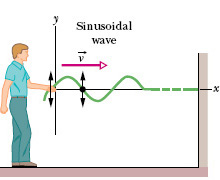
\includegraphics[width=0.3\textwidth]{fig_16_1.jpeg}
  \caption{(a) A single pulse is sent along a stretched string. A typical string element (marked with a dot) moves up once and then down as the pulse passes. The element’s motion is perpendicular to the wave’s direction of travel, so the pulse is a transverse wave. (b) A sinusoidal wave is sent along the string. A typical string element moves up and down continuously as the wave passes. This too is a transverse wave.} \cite{Halliday_Resnick_Walker_2005}
  \label{fig:transverse-wave-longitudinal-wave}
\end{figure}

Simple tones, such as sine waves and cosine waves, are transverse periodic waves which are singular in frequency. These waveforms, as mentioned, are the simple waveforms which compose the building blocks of more complex sounds (waveforms). Arbitrarily, we choose the sine wave to serve as an example of \textit{superposition}, defined as the concept in which two or more waves pass simultaneously through the same region \cite{Halliday_Resnick_Walker_2005}, and several effects may occur simultaneously as their net effect is the sum of the individual effects. Suppose we have two waves which are traveling simultaneously through the same stretched string, and let $y_1(x, t)$ and $y_2(x, t)$ be the displacements the string will experience if each wave were to travel alone the wave alone. The total displacement of the string when the waves overlap will then be

\begin{equation}
	y'(x, t) = y_1(x, t) + y_2(x, t)
\end{equation}

Occasionally, multiple sinusoidal waves of the same wavelength and amplitude moving in the same direction may \textit{interfere} with each other, as the superposition principle applies. The resultant wave of this interference depends on the extent to which the waves are in phase/in step with respect to each other. If the phase of both waves are exactly the same (``in phase,'' in which the peaks and troughs of each wave is the same) then the total displacement is doubled from the displacement of each individual wave. On the other hand, if both waves are exactly ``out of phase'' (the peaks of one wave is the exact same as the troughs of the other) then the total interference will result in the cancellation of noise, as each wave will fully cancel the other \cite{Halliday_Resnick_Walker_2005}. This is how much of the ``noise-cancelling'' technology works in headphones and speakers, in which the phases of multiple waveforms combine to cancel each other, resulting in the perception of no noise. As in Equation \ref{eq:noise-cancelling}, suppose $y_1(x, t)$ is the displacement of $y$ of one wave, and $y_2(x, t)$ be the displacement of another wave. 

\begin{equation}
	\begin{aligned}
	y_1(x, t) &= y_m\sin(kx - \omega t) \\ 
	y_2(x, t) &= y_m\sin(kx - \omega t + \varphi)
	\label{eq:noise-cancelling}
	\end{aligned}
\end{equation}

Waves $y_1(x, t)$ and $y_2(x, t)$ have the same angular frequency $\omega$ (and thus also the same temporal frequency $f$, the same angular wave number $k$ (and thus also the same wavelength $\lambda$), and amplitude $y_m$. Both waves travel in the positive direction of the x-axis, at the same speed. The only difference between the two waves is the phase shift $\varphi$, resulting in the two waves being out of phase, and cancelling the noise of the resultant wave.

\subsection{Sine Waves}\label{subsection:sine-waves}
The first of the basic periodic waves is the sine wave, and is the most common type of periodic wave. The sine wave is a signal with only one frequency, and represents the unidimensional motion for any signal with a phase angle that rotates at a constant rate. It is also based on the trigonometric sine function. On the unit circle, the trigonometric sine function of a phase angle $\theta$ is defined as the ratio of the length of the opposite side and the hypotenuse of a right triangle. The unit circle, with a radius of 1, results in the sine function $sin\theta$ being equal to the y-value in Cartesian coordinates, where the hypotenuse of the right triangle that is formed meets the circle, like in Figure \ref{fig:unit-circle}. We can then use this trigonometric sine wave to synthesize a sine wave audio signal. As sine wave is a continuous periodic wave, in which the wave continues to sound until stopped, we must use the sine wave function on the unit circle continuously. Thus, we use the sine function continuously around the unit circle, going counterclockwise. We notice that in the correlation between Figures \ref{fig:basic-sine-wave} and \ref{fig:unit-circle} moving counterclockwise through the unit circle results in the appropriate rise and fall of the sine wave. $\frac{\pi}{2}$ is the highest y-value within the Cartesian plane, and so denotes a peak in the sine wave, while $\frac{3\pi}{2}$ is the lowest, denoting a trough.

\begin{figure}[h]
	\centering
	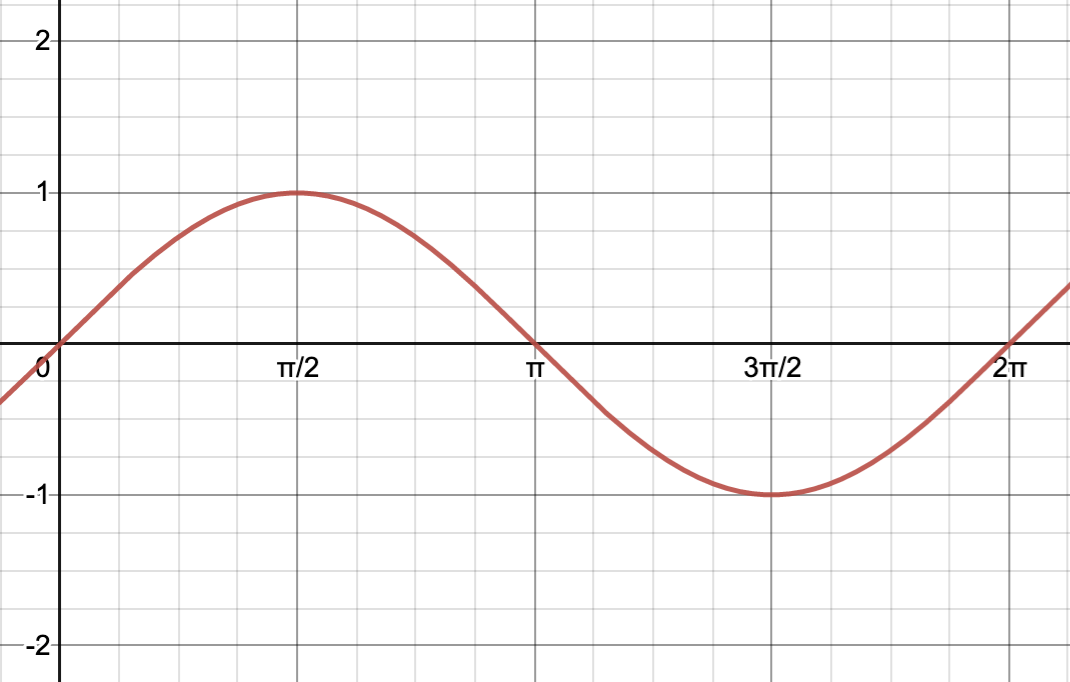
\includegraphics[width=0.5\textwidth]{figures/sine-wave-form.png}
	\caption{A basic sine wave}
	\label{fig:basic-sine-wave}
\end{figure}

\begin{equation}
	y = Asin(B(x + C)) + D
	\label{eq:sine-wave-equation}
\end{equation}

Like with the other periodic waves, sine waves have three important properties: frequency, amplitude, and phase. From the generic function for a sine wave as in Equation \ref{eq:sine-wave-equation}, we are able to compute the various properties. First, \textit{A} is the sine wave's amplitude. This is defined as the height from the center line of the wave to its peak or trough. For our unit sine wave, this value will be 1. Second is the variable \textit{B}, which helps to define the period of the wave, or the distance between one peak and the next, or one trough and the next. With Equation \ref{eq:sine-wave-period}, we see the period is equivalent to taking the total circumference of the unit circle, and dividing it by \textit{B}. Third, the phase shift of a sine wave is denoted by \textit{C}. If the expression is $(x + C)$, then the phase of the sine wave will shift to the left, as the x-value of the wave becomes negative \textit{C}. Otherwise, if the expression is $(x - C)$, then the wave will shift right, with a positive x-value as \textit{C}. Finally, the variable \textit{D} is equivalent to the vertical shift of the wave. This notates the distance that the wave will shift vertically from its unit circle position. As sine waves are only composed of a fundamental frequency, these waves are most used as pure sound tones. Sine waves are a center point of audio synthesis and sound analysis. Other, more complex, periodic waves can be built using some combination of sine waves. 

\begin{equation}
	\frac{2\pi}{B}
	\label{eq:sine-wave-period}
\end{equation}

\begin{figure}
	\centering
	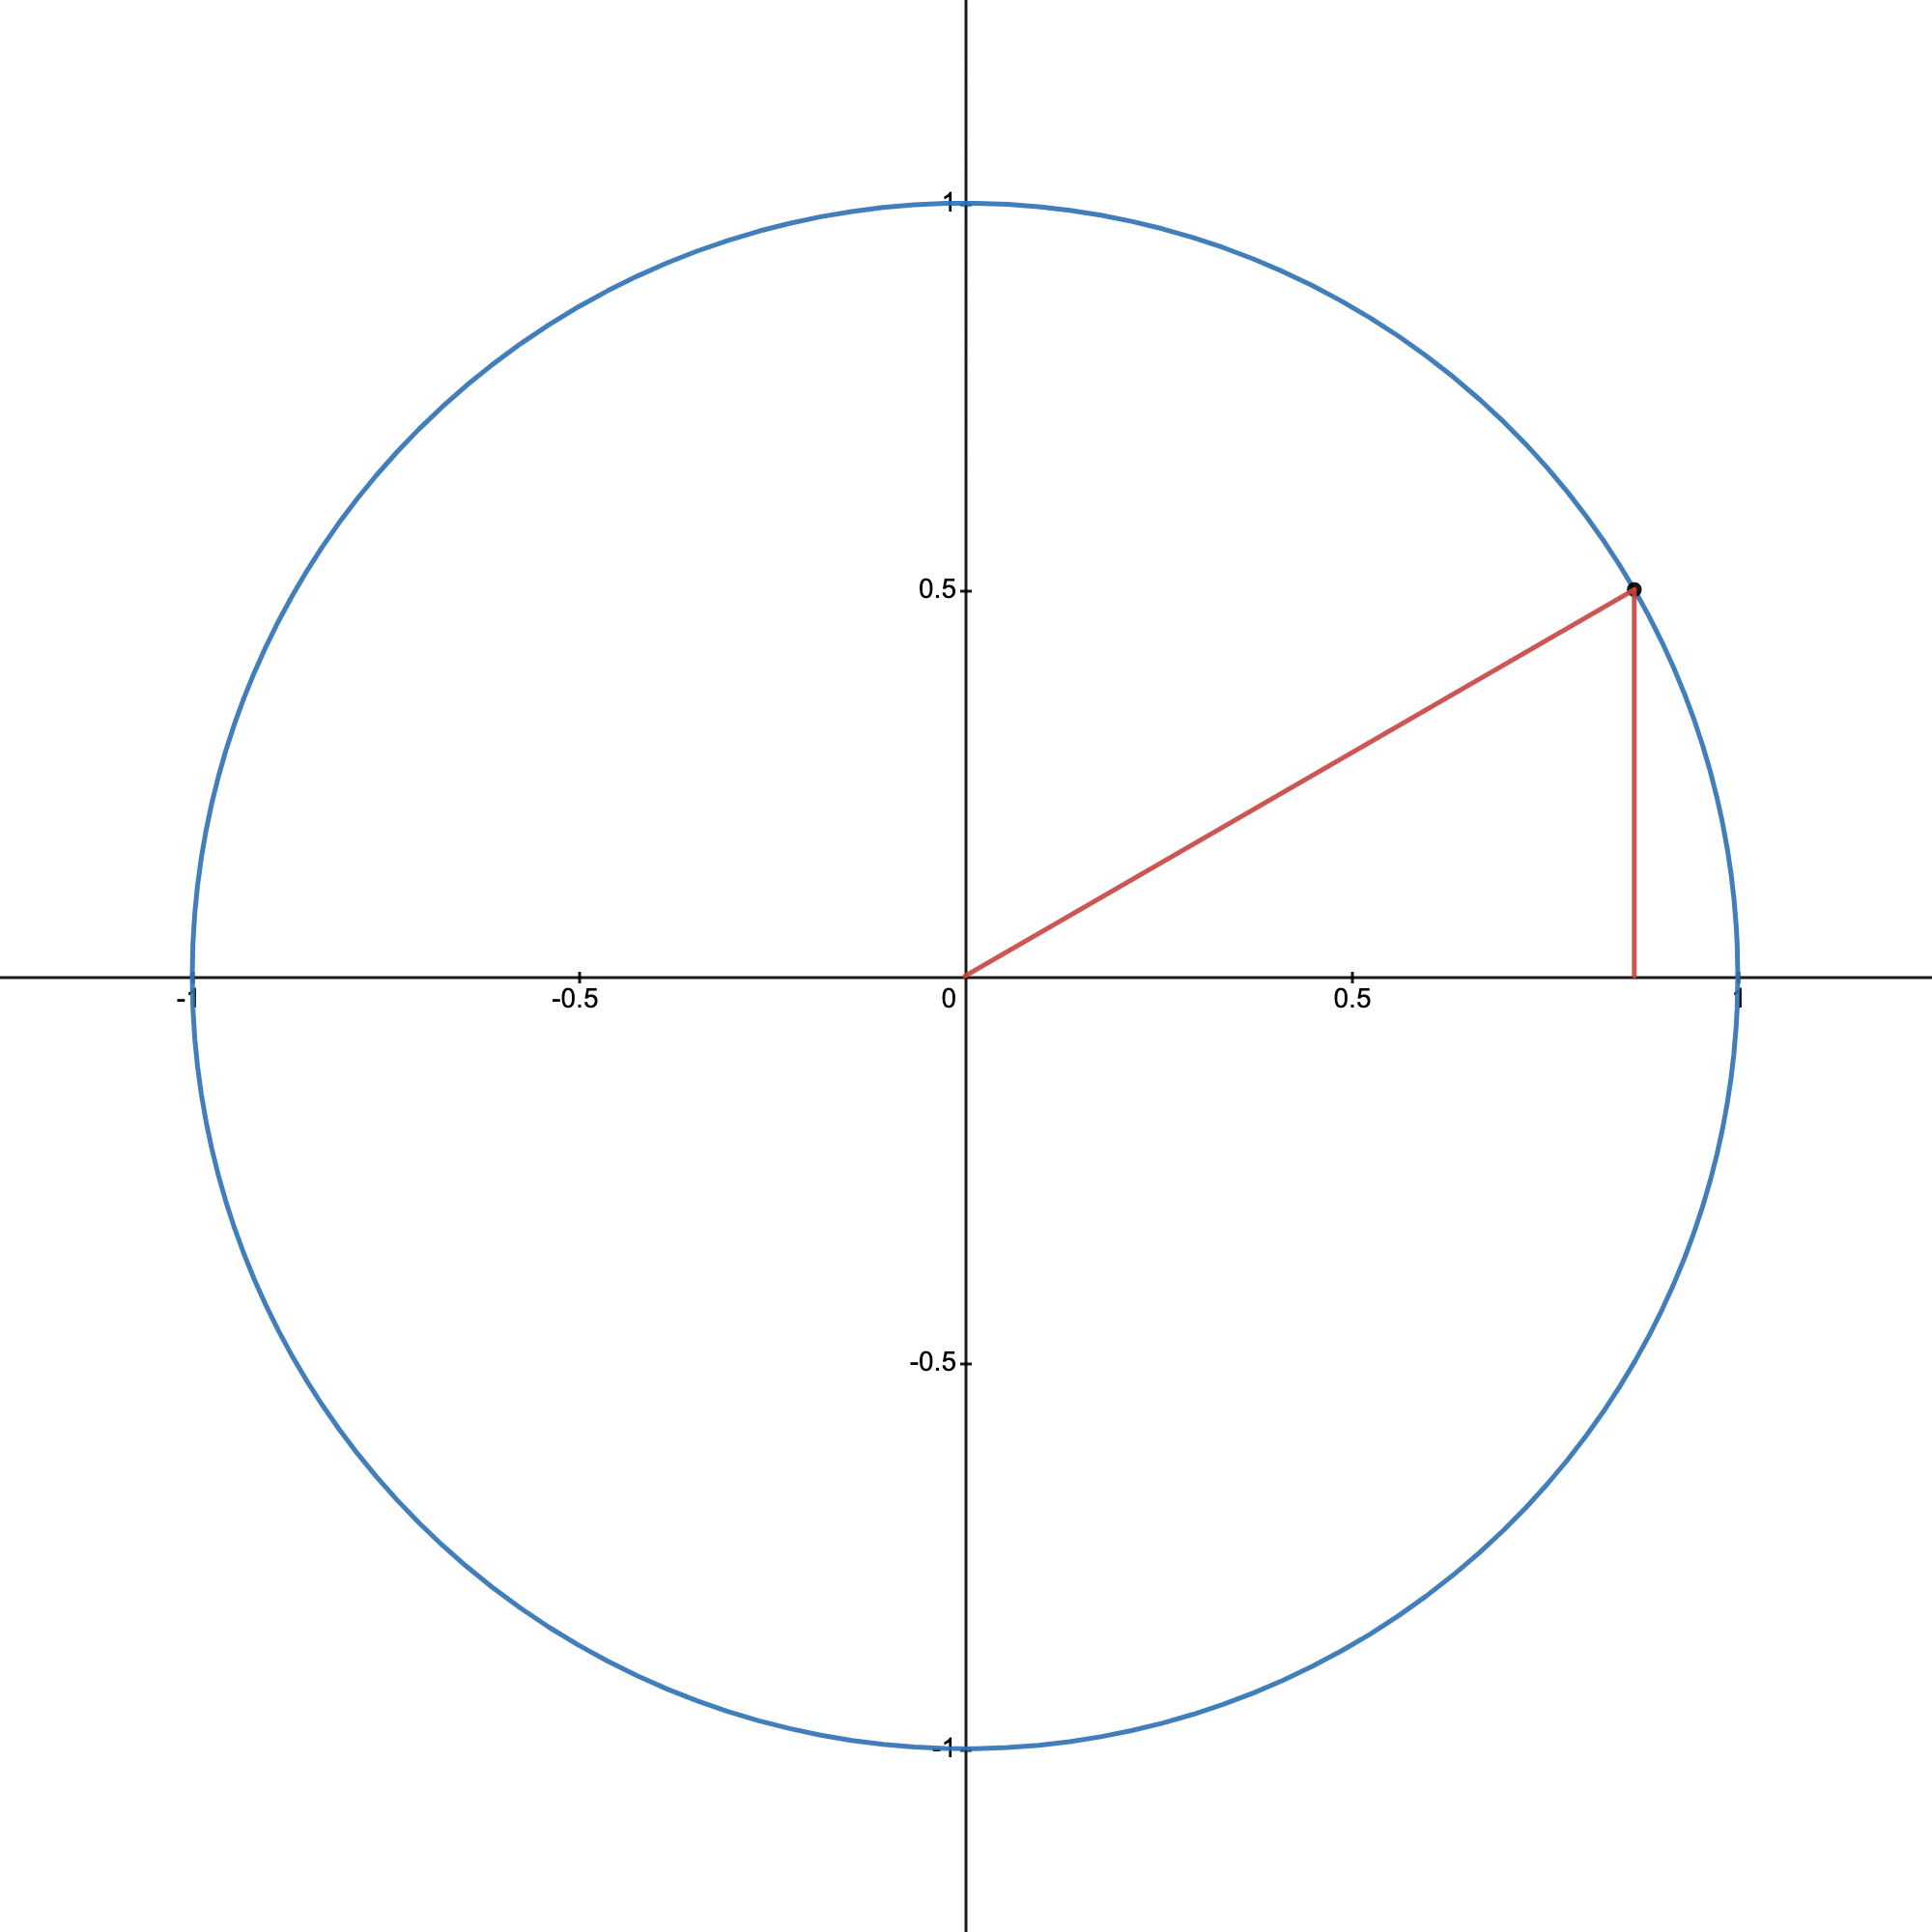
\includegraphics[width=0.5\textwidth]{figures/unit-circle.png}
	\caption{The unit circle}
	\label{fig:unit-circle}
\end{figure}

\subsection{Square Waves}

The square wave is a certain type of pulse wave which allows for a frequency to sound at fixed amplitudes for an arbitrary duration. At its simplest, a square wave can be defined as a sign function of a sinusoidal. A sign function, or a signum function, as in Figure \ref{fig:sign-function}, is an odd mathematical function which extracts the sign of a real number, expressed as $sgn$. Of a real number $x$, it is a piecewise function, defined as in Equation \ref{eq:sgn-function}. So, the square wave is only able to contain odd harmonics, given by its nature of being a type of signum function. Potential harmonics which are not odd or do not fall within exact odd multiples of an arbitrary frequency will cause the wave to become non-square \cite{Case_2007}.

\begin{figure}[ht]
  \centering
  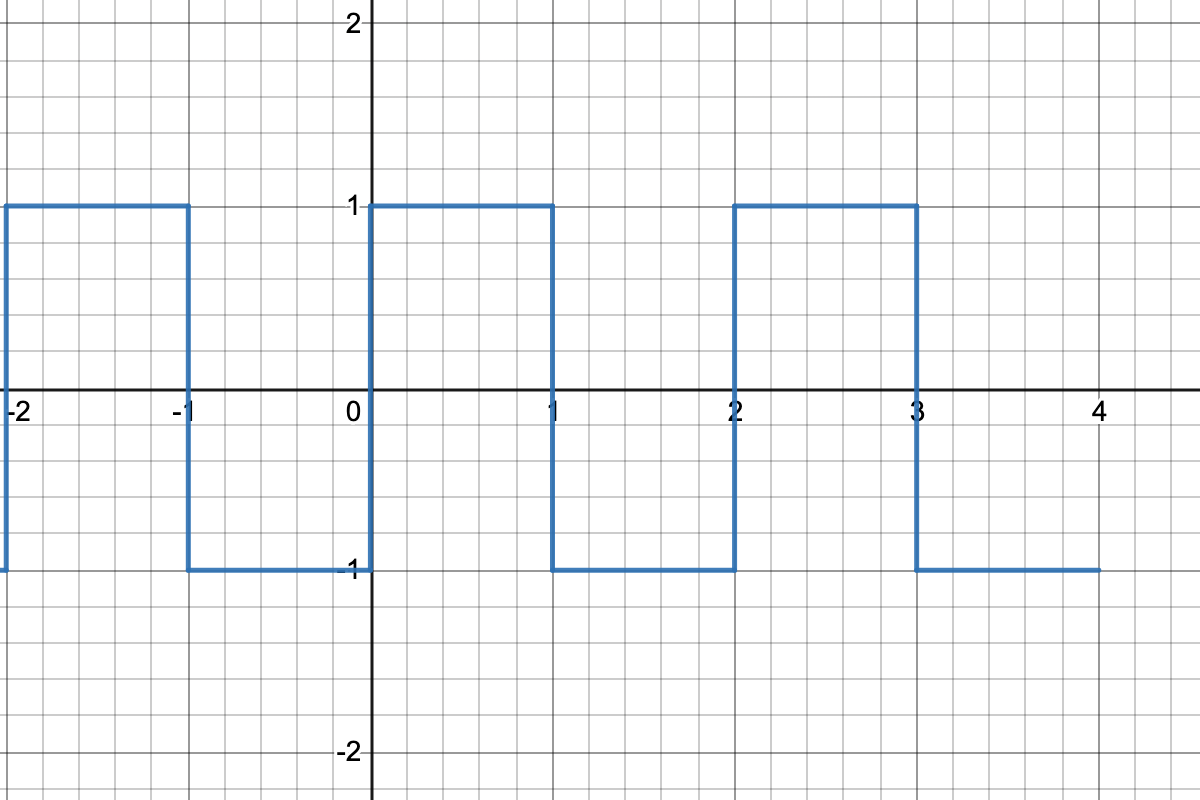
\includegraphics[width=0.5\textwidth]{square-wave.png}
  \caption{A basic square wave}
  \label{fig:square-wave}
\end{figure}

\begin{equation}
	sgn (x): \begin{cases}
		-1 & \textrm{if } x < 0, \\
		0 & \textrm{if } x = 0, \\
		1 & \textrm{if } x > 0
	\end{cases}
	\label{eq:sgn-function}
\end{equation}

\begin{figure}[ht]
  \centering
  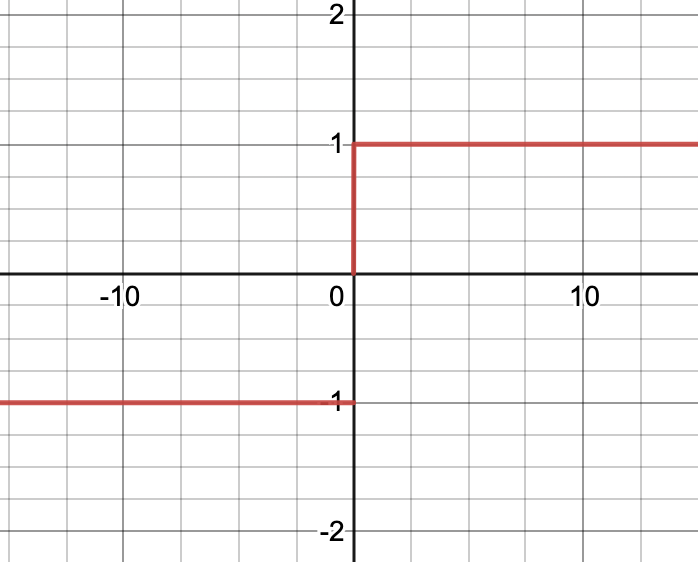
\includegraphics[width=0.5\textwidth]{sign-function.png}
  \caption{A sign function}
  \label{fig:sign-function}
\end{figure}

Thus, we have a square wave equal to Equation \ref{eq:square-wave-function}. The function $x(t)$ will equal 1 when the sinusoidal is positive, -1 when negative, and 0 at the discrete values where the sinusoidal is equivalent to 0. Other aspects of the formula can be altered, similarly to how the function for the sine wave is modified, to produce sound changes. The variable $f$ can be modified like how a period for a sine wave is (variable $B$), in which a larger value, as long as the new value is odd, is able to cause a different frequency result over time \texttt{t}. Amplitude can be increased by multiplying our $A$ value, in Equation \ref{eq:square-wave-function} notated as $sgn$, by some arbitrary odd value. This will increase the value of the amplitude, or the value of $x(t)$ to some other value greater than $+1$ and less than $-1$. Finally, we are also able to modify the period of a square wave, multiplying an odd value by our variable $B$, or $\sin(2\pi)$ \cite{Case_2007}.

More simply, the square wave function can be expressed as an arbitrary summation function of an infinite set of sine waves. Using variables $f$ (frequency), $A$ (amplitude), and $n$ number of harmonics, let $f(x)$ be an arbitrary square wave as a function of time $t$ in Equation \ref{eq:square-wave-summation}, with $n = 2i - 1$, positive values for $i$ produce the odd harmonics of triangle waves. Other changes to $f$, $A$, and $n$ would produce other sound output changes \cite{Wellesley_College_Staff_2021}.

\begin{align}
	x(t) = sgn(sin2\pi ft)
	\label{eq:square-wave-function}
\end{align} 

\begin{equation}
	f(x) = A\sum_{i=1}^{\infty}\frac{\sin(2\pi nft)}{n}
	\label{eq:square-wave-summation}
\end{equation}

The sound produced by a square wave is one that is harsh and bright, that is a sound which has many frequencies in the higher frequency ranges (bright), and lacks much of the lower end of the frequency ranges (harsh). In combination, this results in a sound that becomes grating to hear after some time, and introduces listening fatigue. These waves also only contain odd harmonics, so are most used for woodwinds and reeds \cite{Dowsett_2016}. 

\subsection{Sawtooth Waves}
The sawtooth waveform is also a non-sinusoidal wave, which resembles the teeth of a plain-toothed saw. Similar to the square wave, a sawtooth wave will ramp upwards to a peak amplitude height, then sharply drop to its trough, as in Figure \ref{fig:basic-sawtooth-wave}, creating Equation \ref{eq:sawtooth-sinusoidal-function}, with $frac(x)$ referring to what is in Equation \ref{eq:sawtooth-piecewise-function}, as the fractional part of the equation. 

\begin{equation}
	S(x) = Afrac(\frac{x}{T} + \phi)
	\label{eq:sawtooth-sinusoidal-function}
\end{equation}

\begin{equation}
	frac(x) = x - \lfloor x \rfloor
	\label{eq:sawtooth-piecewise-function}
\end{equation}

\begin{figure}[ht]
  \centering
  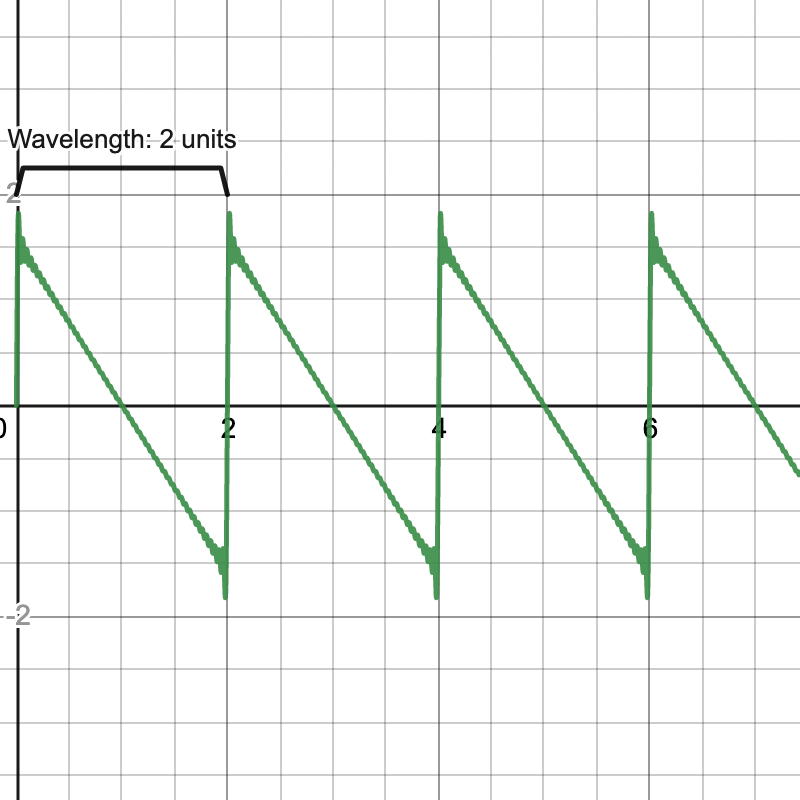
\includegraphics[width=0.3\textwidth]{figures/sawtooth-wave.png}
  \caption{A basic sawtooth wave}
  \label{fig:basic-sawtooth-wave}
\end{figure}

The function $frac(x)$ gives the fractional (or non-integer) part of an arbitrary real number $x$ \cite{Weisstein}. Let $\lfloor x \rfloor$ be defined as the greatest integer which is less than or equal to a real number $x$. Thus, the fractional part of $x$ will be $frac(x) = x - \lfloor x \rfloor$, as seen in Equation \ref{eq:sawtooth-piecewise-function}. For both nonnegative and negative real numbers, $frac(x)$ will be a positive value.

Like with other waveforms, the variable \textit{A} represents the wave's amplitude, and \textit{T} represents the wave's period. The variable $\phi$ denotes the wave's phase, with positive values causing a shift to the left, and negative values a shift to the right. Sawtooth waves are typically created through additive synthesis, much like square waves are, and so we notice that sawtooth waves and square waves have similar periodic equations \cite{Tarr_2019}.

Alternatively, the function for a sawtooth wave can be expressed as the summation of an infinite set of sine waves (which combined, can create a singular sawtooth wave). For Equation \ref{eq:sawtooth-summation-function}, let $f(x)$ be a sawtooth wave as a function of $t$ time in seconds, with frequency $f$, amplitude $A$, and $n$ many harmonics \cite{Wellesley_College_Staff_2021}. Adjustments to this functions can easily be done through modifying the values of $f$ and $A$.

\begin{equation}
	f(x) = \sum_{n=1}^{\infty} \frac{A}{n}\sin(2\pi fnt)
	\label{eq:sawtooth-summation-function}
\end{equation}

Within physical musical instruments, sawtooth waves are most often found within the playing of a string instrument, such as the violin, viola, or cello. As a bowed string oscillates, the bow alternates, in an up-down motion, sticking to the string. The bow will drag the string along as it plays, then slips to allow the string to return to its neutral position \cite{Kapur_Cook_Salazar_Wang_2015} Thus, the nature of the sawtooth wave gives it a bright and energetic sound, and contains both even and odd harmonics. Due to this, sawtooth waves will be used for a variety of instruments, such as strings, brass, pads, and basses \cite{Dowsett_2016}. 


\subsection{Triangle Wave}

A triangle wave is also a non-sinusoidal waveform, named for its triangular shape. Like with square waves, this type of wave only contains odd harmonics, i.e. only containing valid values which are odd numbers. It also shares similarities to the sawtooth wave. In a sawtooth wave, the amplitude of the wave will increase linearly, from a set minimum value (usually 0) to the set maximum value. When the wave reaches this maximum value, the amplitude will immediately return to the minimum value, to begin a new period, or new cycle. Instead, triangle waves will decrease the amplitude of the wave once the maximum value is achieved, as seen with $sin(\pi x)$ in Equation \ref{eq:triangle-wave-function}, until the amplitude reaches the minimum value \cite{Tarr_2019}, as in Figure \ref{fig:triangle-wave}.

\begin{figure}[ht]
  \centering
  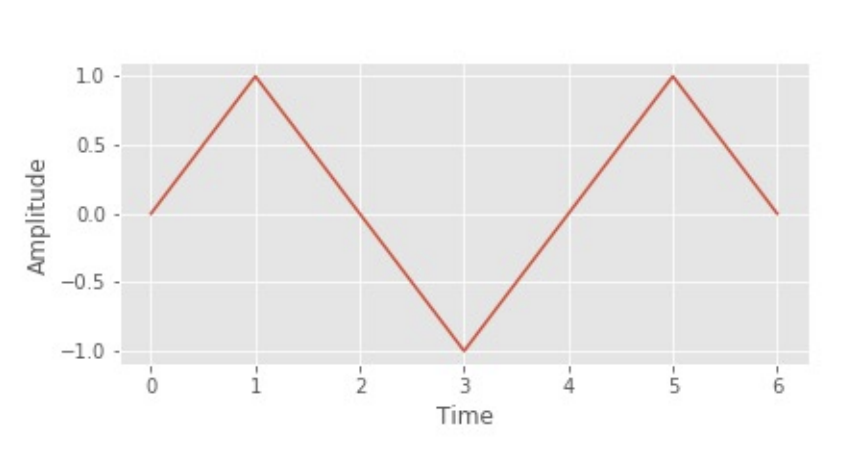
\includegraphics[width=0.4\textwidth]{triangle-waves.png}
  \caption{A basic triangle wave}\cite{Wellesley_College_Staff_2021}
  \label{fig:triangle-wave}
\end{figure}


Like with the other waveforms mentioned, triangle waves can be written as the summation of sine waves. Let $f(x)$ be any triangle wave as a function of time $t$ in seconds, with frequency $f$, amplitude $A$, and $n$ many harmonics, with $n = 2i - 1$. Thus, Equation \ref{eq:triangle-summation-function} will indicate the cycles of a triangle wave. Through adjustments to variables $f$, and $A$, various sound output changes can be achieved. 

\begin{equation}
	f(x) = \frac{2}{\pi}sin^{-1}\lceil sin(\pi x) \rceil
	\label{eq:triangle-wave-function}	
\end{equation}

\begin{equation}
	f(x) = \sum_{i=1}^{\infty} (-1)^i \frac{A}{n^2} \sin(2\pi fnt)
	\label{eq:triangle-summation-function}
\end{equation}

Triangle waves are also ``soft'' sounding waveforms, which decrease in sound faster than some other types of waves. This results in triangle waves being used for piano and flute sounds, as well as other instruments which rely on a quick decay of a note \cite{Dowsett_2016}.

\section{Representing Sound Digitally}

We now understand the physics and mathematics behind sound waves. However, sounds in real life are not composed of simple pure waveforms; sounds in the world around us are made up of multiple harmonics and frequencies layered on top of one another to produce the composite sound which we hear. Sound, like electricity and light, is a form of energy in which molecules in air vibrate and move in a wave pattern. This wave pattern produces the sound waves \cite{Au-Yeung_2021}. Air is able to support multiple sound waves simultaneously, explaining our ability to hear different sounds at the same time. This sound energy is dispersed outwards from the sound source, and will continue to move until the molecules run out of energy, as the energy weakens the further it moves away from the sound source. The sound energy is transferred between molecules, as each molecule moves from an original resting point, transfers energy to another molecule, then returns to its resting point, as in Figure \ref{fig:graphical-rep-vs-physical-sound}. This molecule movement is the oscillation of sound. Molecules become closer together when vibrating, and crowd together in certain places, and thus there are fewer molecules in other places. This visualization of crowds of molecules can be done as a wave, with the peak of a sound wave indicating that there are more molecules together in space (compression of air molecules), and the trough of a sound wave indicating there are fewer molecules (rarefaction) \cite{Toft_2020}. Typically, sound is visualized in a graphical format, with peaks and troughs to a wave rather than drawings showing the compression and rarefaction of air molecules. 

\begin{figure}
  \centering
  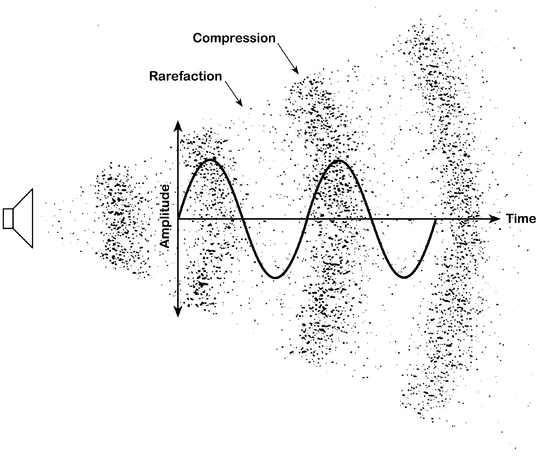
\includegraphics[width=0.4\textwidth]{graphical-rep-vs-physical-sound.jpeg}
  \caption{A graphical representation of sound, vs its physical phenomenon}\cite{Toft_2020}
  \label{fig:graphical-rep-vs-physical-sound}
\end{figure}

Through this periodic nature of waves, the repetitions create what we will recognize to be musical sound, but lacking the specific tonality and timbral qualities of specific instruments. Musical instruments generate a composite set of frequencies, arranged as a layered set of harmonics above the fundamental frequency (the lowest frequency which is played). Thus, the fundamental frequency will be the pitch of the note, and the additional harmonics (also known as overtones) will lie above this pitch and add the tonality or timbre of the note \cite{Toft_2020}. This is what differentiates pure sound waveforms from notes generated from musical instruments, as pure sound waveforms all have pitch, but lack specific timbral quality.\footnote{This is what gives pure sound waveforms their name, ``pure tones,'' as each of these waveforms has pitch but no timbre.} Another factor which dictates what a sound wave will be perceived as is the amplitude of a wave. The wave's amplitude is the distance from the middle of a wave to its crest (peak or trough). Amplitude is also known as the sound's volume, as adjusting the amplitude of a wave will result in a louder sound, and will be further discussed in Section \ref{section:manip-waves}.

To get from an analog sound wave to a digital sound signal, we must sample the continuous analog wave into its digital representation. While an audio signal or sound is a continuous set of values, which are able to be displayed on an oscilloscope (a tool to show oscillations) as a waveform, the digital ``signal'' is a series of numbers, representing various discrete values from the continuous wave. These numbers will represent the values of an audio signal at specific points in time, and are known as \textit{samples} \cite{Russ_2012}. The sampling process to convert from analog (physical) waves to a digital signal involves three steps:

\begin{enumerate}
	\item The audio signal is ``sampled.''
	\item The sample value is converted into a number.
	\item This number is presented at an output port.
\end{enumerate}

The process of sampling will typically produce numbers which are an incomplete representation of the original audio sound, but through careful sampling, this amount of incompleteness can be made insignificant. This same process can be reversed to convert from a digital signal to an analog one, and is known as ``sample replay.'' Sample replay also has three stages and serves as the basis for digital synthesizers, as the conversion from digital signal to analog wave produces the sound that is heard:

\begin{enumerate}
	\item A number is presented to an input port.
	\item This number is converted into an analog signal.
	\item The analog value forms part of an audio signal.
\end{enumerate}

Analog sound exists in two dimensions: time (a period of each wavelength) and space (the displacement of each waveform from the atmospheric pressure). So it makes sense that to convert from analog audio to digital signals, we use these two dimensions: time (\textit{sample rate}) and space (\textit{bit depth}). 

\textit{Sample rate}, or \textit{sample frequency}, is the number of samples which are captured per period (which is commonly measured in Hertz). Typically, digital audio samples of analog audio waves are taken at a rate of 8,000 times per second, or more \cite{Zjalic_2021}. Occasionally, a sound will be sampled that is at a frequency rate higher than 8,000 and the system doing the sampling is unable to identify two points on the waveform to understand the period. Harry Nyquist (1879-1976) was a Swedish physicist and electrical engineer who solved this problem, through the \textit{Nyquist frequency} (or \textit{folding frequency}). Nyquist discovered that in order for an analog audio wave to be accurately represented by a digital signal, and thus also the system which is sampling the audio wave, the wave must be sampled at least twice per wavelength, known as the \textit{Nyquist Theorem} (or \textit{Nyquist-Shannon} theorem) \cite{Zjalic_2021} and visualized in Figure \ref{fig:nyquist-sampling-theorem}. Thus, for a given sample rate, the highest frequency within a system cannot exceed half this sample rate. In other words, the Nyquist frequency is the frequency at 50\% of the sample rate. Otherwise, for a frequency which does not satisfy the requirements for the Nyquist Theorem, a phenomenon called ``aliasing'' would occur, in which signals that exceed half the sample rate are misrepresented as ``alias signals.'' An ``anti-aliasing'' filter would then typically be applied to the signal before sampling occurs, to act as a low-pass filter with a cut-off at the Nyquist frequency. 

This sampling process using the Nyquist frquency and anti-aliasing filter is commonly used in digital audio systems (both for professional and consumer usage). Another tool that is commonly used to improve the anti-aliasing filter is \textit{oversampling} \cite{Huber_Runstein_2018}. Oversampling can increase the effective sample rate between 12 and 128 times the original rate, with three primary reasons for this process. Once the sampling stage is complete, this sampled data will be digitally scaled down to a target data rate and bandwidth for further processing and storage.

\begin{enumerate}
	\item Nyquist filters can be expensive, and difficult to design properly. So by increasing the effective sample rate, and the ceiling for this sample rate, a simpler and less-costly filter can be used.
	\item Oversampling typically results in a higher-quality conversion, for both analog-to-digital (A/D) and digital-to-analog (D/A) conversion.
	\item Multiple samples are usually taken of a single sample level, and so the average noise level will be lower.
\end{enumerate}

\begin{figure}[ht]
  \centering
  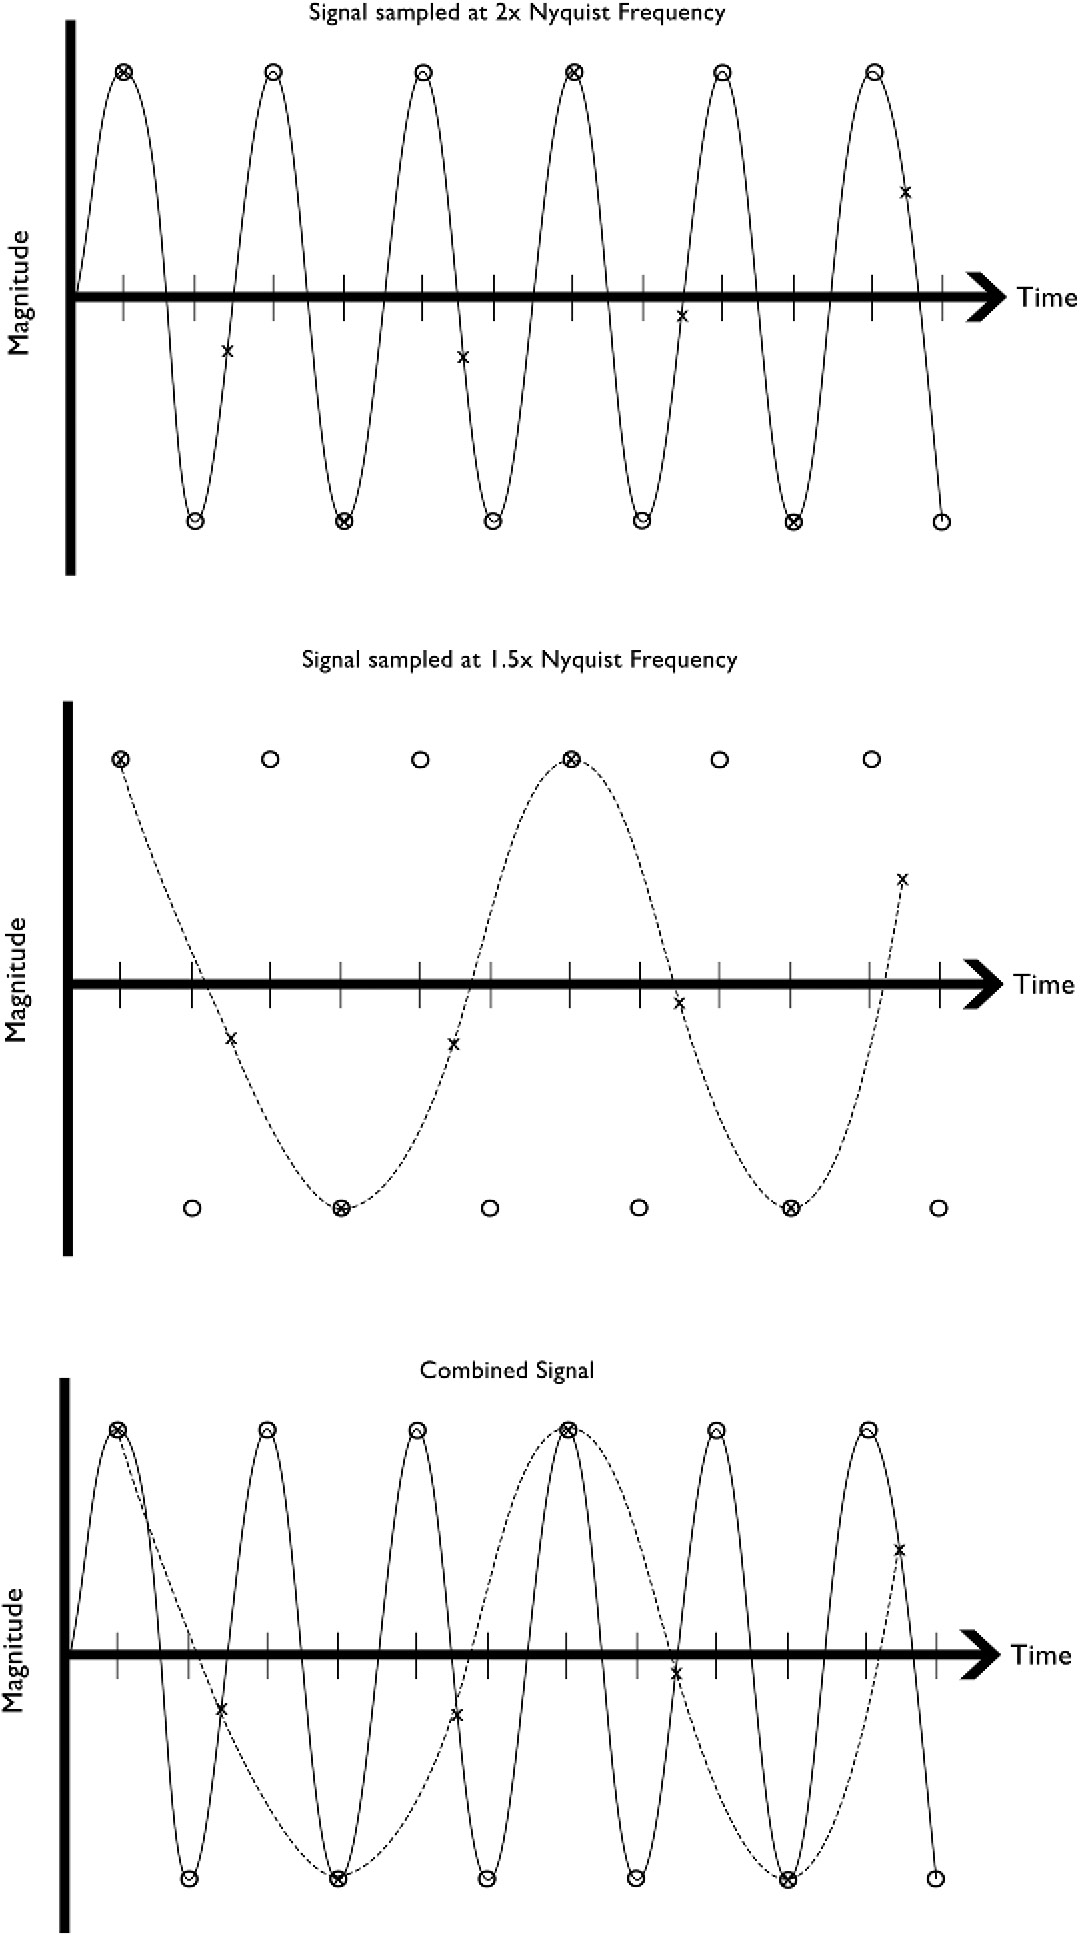
\includegraphics[width=0.5\textwidth]{nyquist-sampling-thoerem.jpeg}
  \caption{The Nyquist sampling theorem visualised. Upper: Signal sampled at 2x Nyquist frequency, Middle: Signal sampled at 1.5x Nyquist frequency (and thus aliasing and not a true representation of the original signal), Bottom: Signal containing both accurate and aliasing components}\cite{Zjalic_2021}
  \label{fig:nyquist-sampling-theorem}
\end{figure}

\textit{Bit depth} is defined as the discrete values which are available within the digital system, representing the magnitude of a continuous electrical signal \cite{Zjalic_2021}, in the form $log_2{x}$. These levels can become exponentially large, and so \textit{quantization} is used, to process data from a broad range into values within a smaller range. It will convert the levels of a continuous analog signal, as the signal after sampling is still in the analog domain, into binary digits (bits). Using bits will allow us to be able to manipulate and store audio data digitally. After sampling the amplitude of an analog audio wave at various precise intervals, we are able to output this amplitude level in its equivalent in bits, which represent the originally sampled amplitude level, known as \textit{bit rates}. The bit ``rate'' can then be defined as the amount of data stored or transmitted per second of time, or in Equation \ref{eq:bit-rate}, measured in kbps \cite{Zjalic_2021}. In general, the higher the value of the bit rate, the higher the quality of the audio data that is stored, since there is more data to represent the captured sound available.

\begin{equation}
	\textrm{bit rate (bits per second)} = \textrm{sample rate (Hz) x } \textrm{bit depth x } \textrm{number of channels}
	\label{eq:bit-rate}	
\end{equation}

From our original three stages of converting analog sound to digital signals, we can now specify the processes which occur in each stage \cite{Huber_Runstein_2018}. Upon playback, the bits are then converted back into analog amplitude values, at precise intervals in time, allowing for the originally recorded amplitude values to be re-created, processed, and played back \cite{Huber_Runstein_2018}. 

\begin{enumerate}
	\item Sampling analog audio wave amplitude levels at precise intervals in time.
	\item Converting these samples into the digital bit value (typically a 16-bit length), which most accurately represents the amplitude levels.
	\item Storing these sample equivalents (the bit values) within digital memory.
\end{enumerate}


\section{Manipulating Sound Waves}\label{section:manip-waves}
As previously mentioned in Section \ref{section:modular-synth-what-is}, modular synthesis involves sending an audio signal through patches or modules in a linear format to achieve the desired sound output changes. To explain how these changes occur to a sound wave, we arbitrarily choose the simple sine wave as an example, as in Figure \ref{fig:sine-wave-period-amplitude}. Sine waves are a waveform which is a function of time \texttt{t}

\begin{figure}[ht]
	\centering
	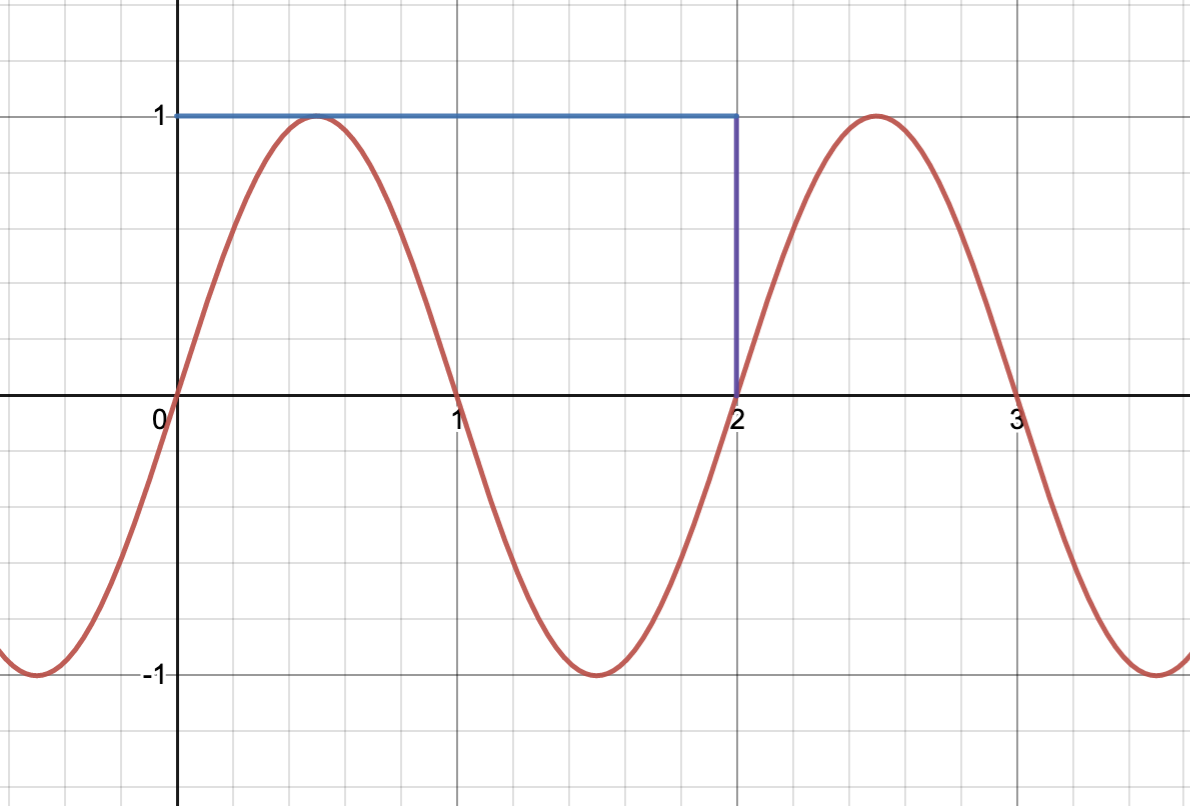
\includegraphics[width=0.3\textwidth]{figures/sine-wave-period-amplitude.png}
	\caption{A basic sine wave, with period demarcated in blue, and amplitude in purple}
	\label{fig:sine-wave-period-amplitude}
\end{figure}

\begin{equation}\label{eq:full-sine-wave-equation}
	y(t) = A \sin(2\pi ft + \varphi)
\end{equation}

with variables $A$, $\varphi$. $A$ is the wave's amplitude, which determines the peak deviation from zero. The frequency is $f$, and $\varphi$ is the wave's phase, which specifies (in radians) where in its cycle the wave's oscillation is at time $t$ \cite{Kirk_Hunt_2013}. When $\varphi$ is not equal to zero, the wave itself will appear to be shifted by the value equal to $\varphi$, which is known as a wave's \say{phase shift.} A negative value will represent a delay in sound, while a positive value will represent an advance in the heard sound.

Thus, there are three primary options when manipulating audio (or a simple waveform); amplitude, frequency, and phase can all be modified at various points to affect the audio output. The first, amplitude, will determine the volume of the wave's sound. The larger the distance between zero and the wave's peak, the louder the human ear will perceive the sound to be\cite{Zjalic_2021}. In Figure \ref{fig:sine-wave-period-amplitude}, amplitude is colored purple, and we see it has a value of 1 (the default value of amplitude of a sine wave from the unit circle), as $A$ does in Equation \ref{eq:full-sine-wave-equation}. By changing the value of $A$ to either $\frac{1}{2}$, or $2$, the peak of the wave will change accordingly, becoming larger or smaller depending on the set value of $A$. This change is reflected in the sound we can hear, as like in Figure \ref{fig:half-sized-sine-wave} and Equation \ref{eq:half-sized-sine-wave}, the volume of this sine wave is halved. Thus, volume ranges can be between soft (at a barely audible \textit{pianissimo}) with an amplitude $A = \frac{1}{2}$, or loud (\textit{fortissimo}), with $A = 4$, for instance.

\begin{equation}\label{eq:half-sized-sine-wave}
	y(t) = \frac{1}{2} \sin(\omega t + \varphi)
\end{equation}

\begin{figure}[ht]
	\centering
	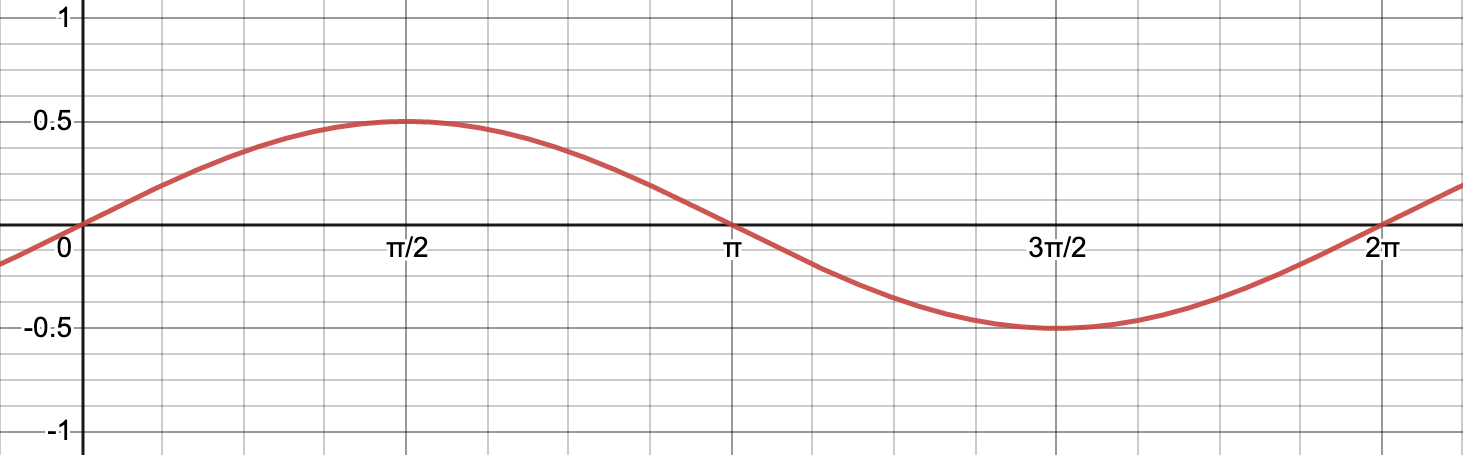
\includegraphics[width=0.5\textwidth]{figures/half-sized-sine-wave.png}
	\caption{A sine wave, with an amplitude of $\frac{1}{2}$}
	\label{fig:half-sized-sine-wave}
\end{figure}

The second option commonly used to manipulate audio is to change an audio signal or wave's frequency. For sound and audio manipulations, the frequency component determines a sound's \say{color,} or \say{timbre.} It is the property of a waveform which determines the output sound's pitch. The high-end of audible frequencies for the human ear is around 20,000 Hz (20 kHz), though this reduces with age. The generally accepted range of human hearing ranges from 20 Hz to 20 kHz, with frequencies below 20 Hz felt more than heard\cite{Rosen_Howell_2011}. This range is further broken down in Table \ref{tbl:frequency-table-of-human-hearing-general} of Appendix \ref{appendix:frequency-table}. Thus, with Equation \ref{eq:full-sine-wave-equation}, we change the value of $w$, which increases the rate of change of the sine wave, increasing the perceived pitch. With the period of the sine wave in Figure \ref{fig:sine-wave-period-amplitude} marked blue, it is this blue section that will increase with an increase in $\omega$. As $\omega$ increases, there are more repetitions of the sine wave's phase, so the audio output's pitch will increase. Pitch is how high or low a sound is perceived to be, and will be determined by the frequency of the vibrations \cite{Toft_2020}. Frequency is the number of wave cycles which pass through a given point per second. A higher frequency will result in a higher pitch, and a lower frequency will result in a lower pitch. For instance, with a frequency of 261 Hz, we perceive the note Middle C to be played. 

Finally, a modification to a wave's phase will determine if the audio signal output is on-time, delayed, or early. The numeric value of $\varphi$ depends on the start of the wave's period. Similar to the changes made to amplitude and frequency, by modifying the value of $\varphi$, we change the phase of the waveform. This will be most noticeable with multiple harmonics or simple waveforms stacked on top of each other, in which each signal will have a phase at a slightly different time, as in Figure \ref{fig:sine-wave-phase-shift}. The period of the blue sine wave has a length of $\frac{\pi}{2}$, but otherwise is a normal unit circle sine wave. The red sine wave is phase shifted, with an $\varphi$ value of positive 2, which shifts the wave negative and to the left, causing the output audio to sound early in comparison to the blue wave. 

\begin{figure}[ht]
	\centering
	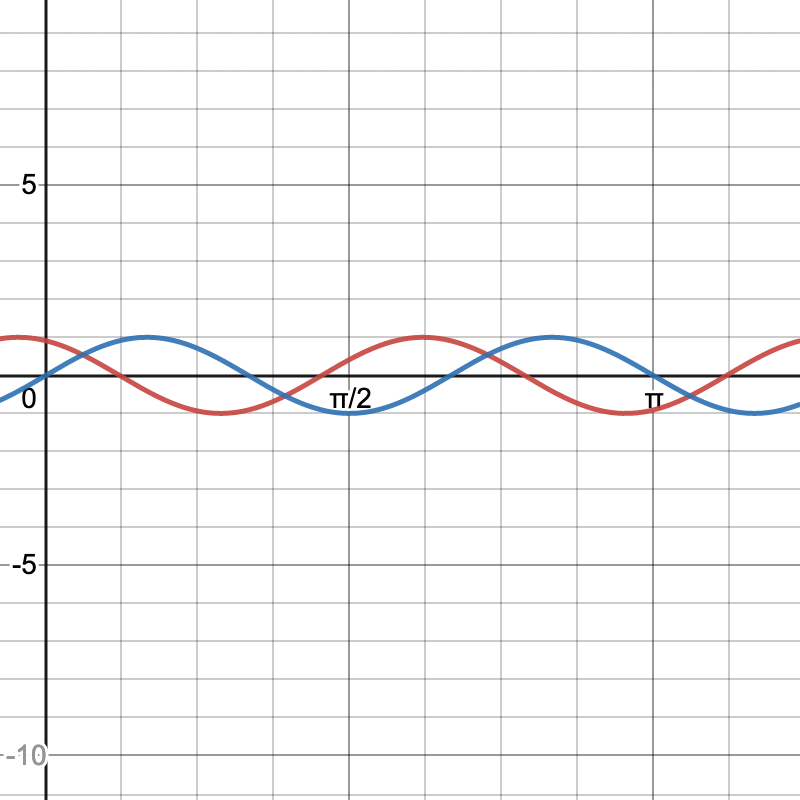
\includegraphics[width=0.5\textwidth]{figures/sine-wave-phase-shift.png}
	\caption{The phase shift in a sine wave}
	\label{fig:sine-wave-phase-shift}
\end{figure}


This type of sound modulation is done through this synthesizer's ``delay'' effect (sometimes known as ``echo'' effect). It is an effect which records an input signal, stores it, then plays it back after a defined time. Typically, the delayed audio is mixed with the live audio input creating an echo effect, where we first hear the original audio, followed by the delayed audio. The value of $D$ in Equation \ref{eq:sine-wave-equation} determines the shift of the wave, and thus also the sound. A positive value (such as $\frac{\pi}{2}$) will shift the sine wave to the left on the Cartesian plane, resulting in a sine wave which sounds early. The same applies to a negative $D$ value, in which a value such as $-\frac{\pi}{6}$ shifts the sine wave to the right, creating a sine wave which sounds ``late'' or delayed.

Other modules can be created through similar logic. To create legato and staccato, we either connect the waves of different frequencies together, or separate the waves to the point there is a clear distinction between the notes. Musically, these two concepts are total opposites; staccato is defined as the style of playing notes in a detached and separated manner, in which each note is clearly distinct from one another. It is typically indicated by a dot directly above or below the notehead, depending on if the stem of the note goes upwards (a dot is placed below the notehead), or goes downwards (a dot is placed above the notehead) \cite{Burkholder_Grout_Palisca_2014}. An example of staccato is in Figure \ref{fig:bartok-dance-five-b-section}, in which there are dots clearly above and below some of the notes, and the location of the dot is dependent on whether the stems of the notes face upwards or downwards. Legato is the directive which defines notes to be played in a smooth and connected manner, with notes that are no longer clearly distinctive from one another, as each note will flow gracefully into the next.

\begin{figure}[h]
  \centering
  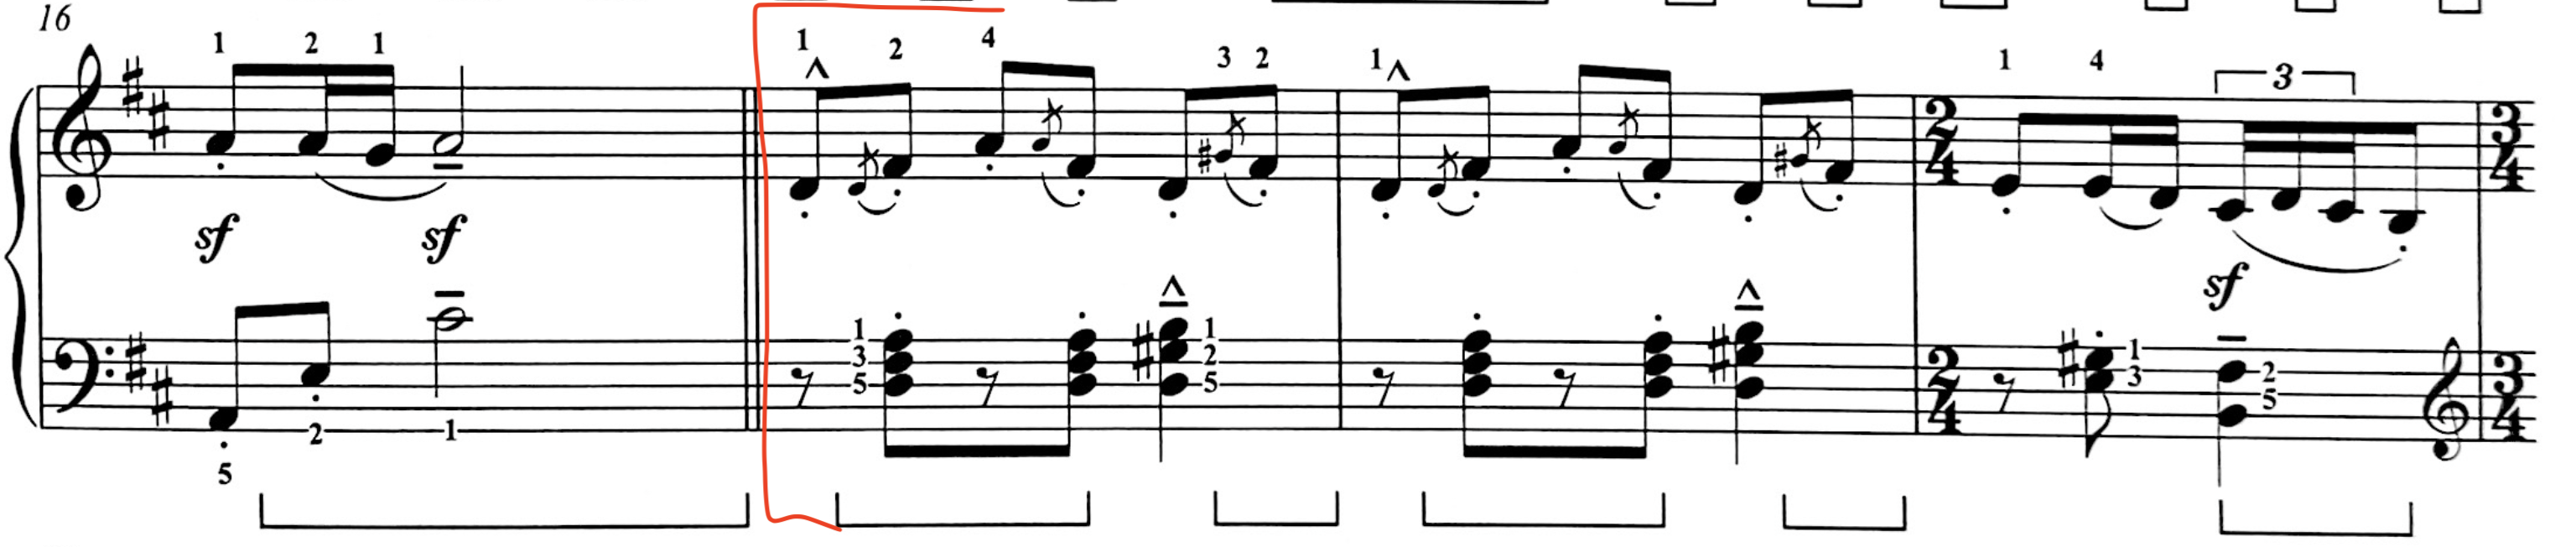
\includegraphics[width=\textwidth]{bartok-dance-five-b-section.jpg}
  \caption{Béla Bartók, Romanian Folk Dances, \textit{Poarga Românească}, mm. 16-19}
  \label{fig:bartok-dance-five-b-section}
\end{figure}

We will also create a module meant to layer specific harmonics over a base frequency: the major third interval, and the perfect fifth interval, which together will form a major chord. A chord can be defined as the simultaneous sounding of two or more notes (typically three or more). Most chords are triadic in nature (that is, containing only three notes), with the interval of a major third or minor third between each of the three notes. The major third interval can be defined as the interval which spans four degrees of the diatonic scale in the Western twelve-semitone tuning system (refer to subsection \ref{subsection:how-midi}), or four semitones \cite{Nave_2017}.\footnote{The major third interval is also enharmonically equivalent to the diminished fourth interval. The enharmonic interval describes notes which sonically are the same, yet notated differently.} The minor third interval contains one fewer degrees than the major third interval, thus having only two degrees of the diatonic scale, and so only three semitones. For instance, the interval between $A$ and $C\musSharp{}$ is a major third, as the note $C\musSharp{}$ lies four semitones away from the note $A$, while the interval between $A$ and $C$ is a minor third, with the note $C$ lying only three semitones away from the note $A$. Notable examples of the major third interval include the first two notes of the song ``When the Saints Go Marching In,'' the first movement of Ludwig van Beethoven's \textit{Fifth Symphony} (Figure \ref{fig:beethoven-fifth} \cite{Beethoven_1862}), or the song ``Swing Low, Sweet Chariot.'' Examples of the minor third interval include the first two notes of the tune of ``Greensleeves,'' (Figure \ref{fig:greensleeves} \cite{Kurtz_2010}) Christmas tune ``What Child is This,'' or The Beatles' ``Hey, Jude.''

\begin{figure}[ht]
  \centering
  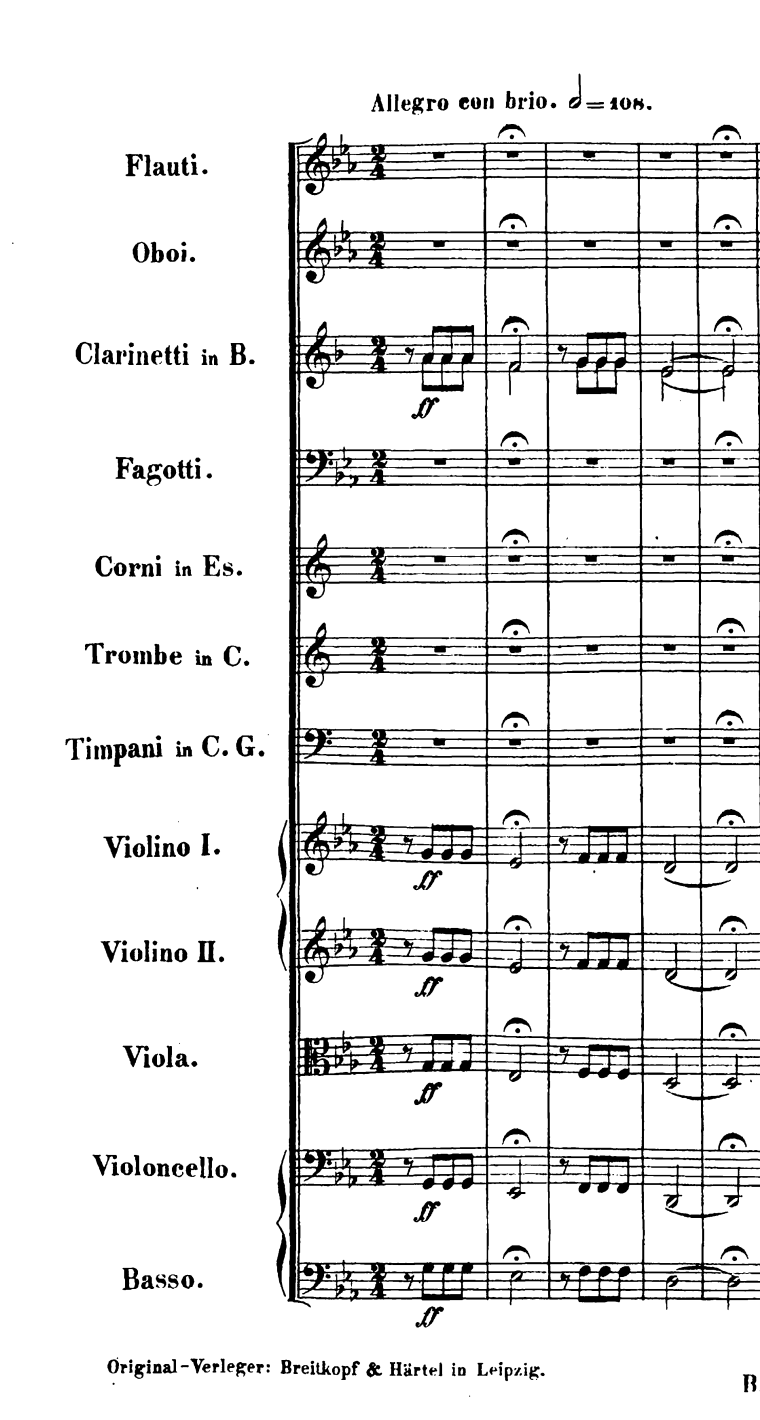
\includegraphics[width=0.5\textwidth]{beethoven-fifth.jpg}
  \caption{Ludwig van Beethoven, Symphony No. 5 in C Minor, \textit{Allegro con brio}, mm. 1-4}
  \label{fig:beethoven-fifth}
\end{figure}

\begin{figure}[ht]
  \centering
  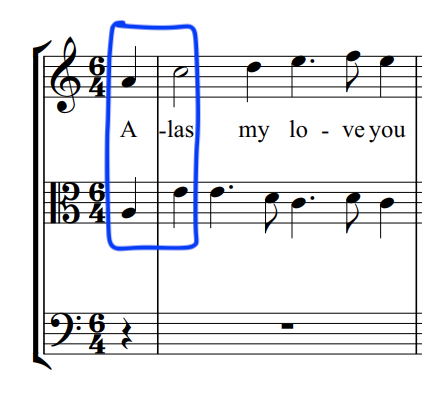
\includegraphics[width=0.4\textwidth]{greensleeves.jpg}
  \caption{``Greensleeves'', mm. 1}
  \label{fig:greensleeves}
\end{figure}

The interval of the third is important to distinguish \textit{major} chords, and \textit{minor} chords, as major chords will have a root note (the tonic note), major third interval, and another minor third interval (or perfect fifth interval above the tonic) stacked on top of one another, while a minor chord will have the tonic, minor third, and perfect fifth. Either multiple waveforms (of the specified major third and perfect fifth intervals) can be stacked to produce the major chord sound, or MIDI inputs can trigger a major chord.

To add the distortion alteration (as opposed to the specific distortion effect) to a sound is simply to add desired textures to a sound, through changing and deforming an audio signal's waveform. For many, a prime example is seen with the use of an electric guitar, as the pedals used with an electric guitar allow for added harmonics, and other changes made to the guitar's sound. One of the most used types of distortion is known as \textit{clipping}, in which the level of a signal (typically amplitude) goes beyond the maximum that a system is able to handle, leading to clipping, as the maximum of the waveforms gets abruptly cut off at the system's maximum. At its best form, distortion can be a gentle audio effect, which can add many types of sounds to a signal, including saturating the sound, and adding overdrive and \textit{fuzz} through adding \textit{gain} (defined as an increase in some type of value). Within the field of distortion, \textit{gain} is referred to as \textit{transmission gain}, in which there is an increase in the power of a signal, expressed in \textit{decibels} (dB), usually done through an arbitrary combination of increasing the amplitude and frequency of a sound wave.

The two most common, and most subtle, types of distortion are saturation and clipping. The result of these two types of clipping is ``soft clipping'' in which the peaks of the signal's waveform are softly rounded, and not abruptly cut off \cite{Tarr_2019}. The signal will be pushed only slightly over the 0 dB threshold. 

The concept of the 0 dB threshold is important, as it is a fundamental aspect of music production and mixing, as well as how to effectively create distortion within a modular synthesizer. Both digital and analog meters for volume, as in Figure \ref{fig:server-meter}, have ranges between negative infinity (or silence), up to 0 dB (the absolute loudest). These decibels are different that the standard decibels used to describe the loudness of everyday sounds. Standard decibels allow us to compare the relative loudness of sounds to each other; a jet taking off sounds at 140 dB, a firecracker is 140-165 dB, and a whisper may be 30 dB \cite{Hearing_Health_Foundation}. These decibels act as a unit measurement for sound, and the National Institute of Occupational Safety (NIOSH) states that while exposure to noise at 85 decibels or above  will cause hearing loss, the exposure dangers for higher levels become exponentially more damaging. While at a noise level of 70 dB would take over 24 hours to cause hearing damage, sound at a level of 115 dB would cause hearing damage at only 28 seconds. The 115 dB volume of a rock concert and symphonic orchestra concert is much more noticeable, especially when comparing to the volume of listening to music on personal devices at maximum volume (105 dB).

The type of decibels used for music production are ``Decibels Full Scale'' (dBFS) when discussing digital music, or ``Sound Pressure Level'' (dB SPL) in the real world. This is the measurement of decibels as it pertains to the levels in an audio recording. Unlike the scale for dB, in which 0 dB is absolute silence, and higher numbers indicate a louder perceived volume, the scale for dBFS is reversed. With the dBFS scale, 0 dB is the maximum level of audio a system can process before it ``clips'' the signal. The lowest detectable level of sound in the system, the ``noise floor,''  can be as low as -150 dB, but is typically between -80 dB and -90 dB. In general, the common range for volume lies between -10 and -18 dB, leaving 10 dB as headroom when combining all audio signals into one master track.

\begin{figure}
  \centering
  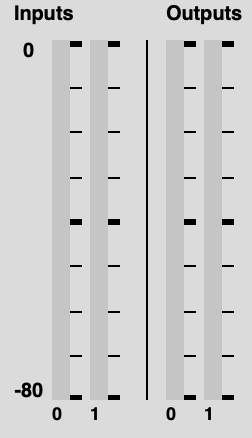
\includegraphics[width=0.2\textwidth]{server-meter.jpg}
  \caption{The server meter in SuperCollider}
  \label{fig:server-meter}
\end{figure}

So, keeping the noise level somewhere between -80 dB and -10 dB will help in introducing distortion to pure sound waveforms. If a signal is ``softly clipped'' (boosted slightly over the 0 dB threshold), the output sound may contain subtle harmonics (other frequencies overlaid on top of the original frequency) or other overtones. 

Overdrive, the distortion effect, and fuzz are three other types of distortion effects, and now are synonymous with electric guitar rigs, pedals, and other similar hardware. Overdrive tends to be the most subtle of the three, with higher gain levels. Distortion and fuzz are more intense, with distortion allowing for large amounts of sustain, harmonics, and a mostly altered sound from the original input, noticeable in heavy rock music and guitar solos. Fuzz is similar to distortion in gain level, but also employs the use of a \textit{frequency multiplier} to produce sound similar to that of a square wave. Distortion using the fuzz effect produces a traditional synth-like effect, with digital artifacts, or overly processed sounds.

\chapter{Building a Modular Synthesizer}\label{chapter:building-a-mod-synth}

In the work done on creating a virtual synthesizer, the result is two input options: pure sound tones (such as the sine waves, square waves, and other waveforms previously mentioned in Section \ref{section:waveforms}), and MIDI. Due to the continuous movement of pure sound waves, modules built for pure tones will be somewhat different from the modules which are built for MIDI input. The following section focuses on the pure sound tones, and the modules built to manipulate these waves. Then, we discuss the ways in which a user can interact with this project's synthesizer through the use of MIDI, and the various sound alterations that result.

\section{The Modules: Pure Waveforms}

The waveforms created through SuperCollider are through Unit Generators (UGens) such as the ``SinOsc'' Unit Generator. As in Listing \ref{lst:sinewave-synthdef}, a simple sine wave is created, with a frequency of 440 Hz ($A_4$, defined as the A in the fourth octave of the keyboard, or Concert A), and a volume of 50. The \texttt{SinOsc} UGen defines the specific properties (frequency, amplitude) of the sine wave, as well as the wave itself. Thus, as previously seen in both Figure \ref{fig:basic-sine-wave} and Equation \ref{eq:sine-wave-equation}, a continuous sine wave has been created.

\begin{listing}
	\begin{lstlisting}
		SynthDef("sinewave", {arg freq=440, vol=50; Out.ar(0, SinOsc.ar(freq, 0, vol))}).add;
	\end{lstlisting}
	\caption{Creating a sine wave SynthDef in SuperCollider}
	\label{lst:sinewave-synthdef}
\end{listing}

\subsection{Volume Slider}
Volume is simply how loud or soft the human ear hears at a particular frequency. The sine wave SynthDef created in Listing \ref{lst:sinewave-synthdef} contains a variable value for volume. In the SynthDef, the volume is initialized at the number 50, which generally correlates to a medium-loud volume of \textit{mezzo forte}. The variable A of the generic sine wave equation in Equation \ref{eq:sine-wave-equation} is equivalent to this change in volume.

As the sine wave Synth Def contains two variables, one for frequency, and one for volume, creating modules for both a volume slider and a pitch knob is straightforward. To create the volume slider, a SuperCollider class called \textit{EZSlider} creates the outline of the volume slider itself, as in Figure \ref{fig:volume-slider-basic}. For the slider's functionality, there are three important parts: the ``controlSpec,'' ``action,'' and ``initVal.'' The ``controlSpec'' defines the ``control spec,'' or the range of values allowed for the specified module. Negative volume does not exist, so this simple volume module will contain valid values for 0 volume (soft, or \textit{pianissimo}) up to 100 volume (loud, or \textit{fortissimo}). Then, the ``action'' argument of the \textit{EZSlider} class determines the function that runs when the value of the volume slider is changed. 

\begin{figure}[h]
  \centering
  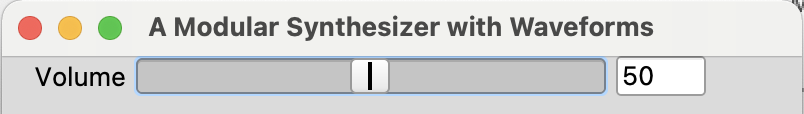
\includegraphics[width=\textwidth]{volume-slider-basic.png}
  \caption{The basic volume slider, with a volume of 50, or \textit{mezzo forte}}
  \label{fig:volume-slider-basic}
\end{figure}

\begin{listing}
	\begin{lstlisting}
		volumeSlider = EZSlider(awindow, label:"Volume", controlSpec:[0,100], action:{|volumeSliderValue| x.set("vol", volumeSliderValue.value)}, initVal:50);
	\end{lstlisting}
	\caption{Creating the volume slider in SuperCollider}
	\label{lst:volume-slider-waveform}
\end{listing}

\begin{listing}
	\begin{lstlisting}
		x = Synth("sinewave");
	\end{lstlisting}
	\caption{Putting the sine wave SynthDef into a Synth, for sound output}
	\label{lst:sinewave-synth}
\end{listing}

In Listing \ref{lst:volume-slider-waveform}, the action that is set involves changing the volume of the Synth created in Listing \ref{lst:sinewave-synth}. In this code example, the SynthDef from Listing \ref{lst:sinewave-synthdef} that is assigned to the variable name ``sinewave'' is now put into a Synth. This Synth, as previously described in Section \ref{section:supercollider}, allows SuperCollider to deal with audio output, as it pushes the created sine wave into the SuperCollider server \textit{scsynth} for immediate playback. So, the SynthDef ``sinewave'' is put into a Synth, known as ``x.'' Within the action, while the sine wave is wrapped in a Synth, $x$ can be manipulated. That is, the sine wave which is in the Synth can be manipulated, resulting in an altered sound. The action itself begins with a reference to the volume slider, $volumeSliderValue$. The Synth, $x$, then references the volume argument from the SynthDef, ``vol,'' which sets the volume for both the SynthDef and the Synth, and uses the \texttt{set} function to set the volume of the Synth equal to the volume that the volume slider contains. The volume of the Synth $x$ will update as the value of the volume slider does, setting the value of \texttt{x.vol} to be equivalent to \texttt{volumeSliderValue.value}. Finally, ``initVal'' simply initializes the starting value of the slider to volume 50 (\textit{mezzo forte}).

\subsection{Pitch Knob: The Pitch Bend}

Pitch, as previously mentioned, is simply a functionality which dictates the frequency of a note that the human ear perceives. Standard Western tuning currently dictates notes to be tuned around the starting pitch of the note A above Middle C (or $A_5$), which is equivalent to 440 Hz. We reference Listing \ref{lst:sinewave-synthdef} again, as a sine wave with both frequency and volume arguments was created here. The frequency of this sine wave is equivalent to the variable \textit{B} in the generic sine wave equation (Equation \ref{eq:sine-wave-equation}).

To create the pitch knob, similar logic to that of the volume slider above is used. In SuperCollider a native class, \textit{EZKnob}, is used. This class will create the knob, as in Figure \ref{fig:pitch-wheel-basic}, to adjust the frequency of the pure tones. This knob class has three arguments: the ``controlSpec,'' ``action,'' and ``initVal.'' In Listing \ref{lst:pitch-knob-waveform}, we see that the controlSpec for the pitch knob is \texttt{freq}, denoting the span of audible frequencies to the human ear, with negative frequencies invalid. The ``action'' argument works similarly to its functionality in the volume slider. It will set the value of \texttt{freq} argument of the SynthDef ``sinewave'' equal to the frequency value of the pitch knob. The final argument of the \textit{EZKnob} class is ``initVal,'' in which the initial value of the pitch knob is set to 440 Hz.

\begin{figure}
  \centering
  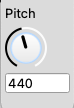
\includegraphics{pitch-wheel-basic.jpg}
  \caption{The basic pitch wheel, with a pitch of 440 Hz, or $A_5$}
  \label{fig:pitch-wheel-basic}
\end{figure}

\begin{listing}
	\begin{lstlisting}
		pitchKnob = EZKnob(awindow, label:"Pitch", controlSpec:\freq, action:{|pitchKnobValue| x.set("freq", pitchKnobValue.value, currentFreq)}, initVal:440);
	\end{lstlisting}
	\caption{Creating the pitch knob in SuperCollider}
	\label{lst:pitch-knob-waveform}
\end{listing}



\subsection{Legato Switch: A Sustain Button}

The \textit{legato} switch for this synthesizer is meant to emulate the \textit{legato} notation found in classical music. \textit{Legato} is a directive, typically found in its full form in classical music, which indicates the performance of a specific passage to be played in a smooth, graceful, and connected style (opposed to the \textit{staccato} notation) \cite{Winer_2018}. It will often be indicated by a slur over the notes, or an accent mark with a line over the notes to be affected, as in Figure \ref{fig:legato-notes-example} \cite{Henle_2009}, marked in blue.

On a physical electronic keyboard, this module is most often seen with a \textit{sustain} button, in which the notes played are extended, and slurred into each other. However, it is important to note that not all slur lines in written sheet music will be meant to be played \textit{legato}. Notes that are to be played \textit{legato} will differ in pitch, connecting notes of different pitches to be played in succession in a smooth manner. This is unlike the notation for tied notes, as in Figure \ref{fig:tied-notes-example} \cite{Lung_2016}, which connect notes that are the same pitch. The durations of the notes which are tied together are combined, and played at that new longer note duration instead. However, further development on this module is not needed. A continuous pure sound wave was created through the SynthDef, and later put into a Synth for sound output. A module to sustain a pure tone and smoothly connect it to the next pure waveform will not alter the output sound of the continuous waveforms which are created within SuperCollider code.

\begin{figure}[h]
  \centering
  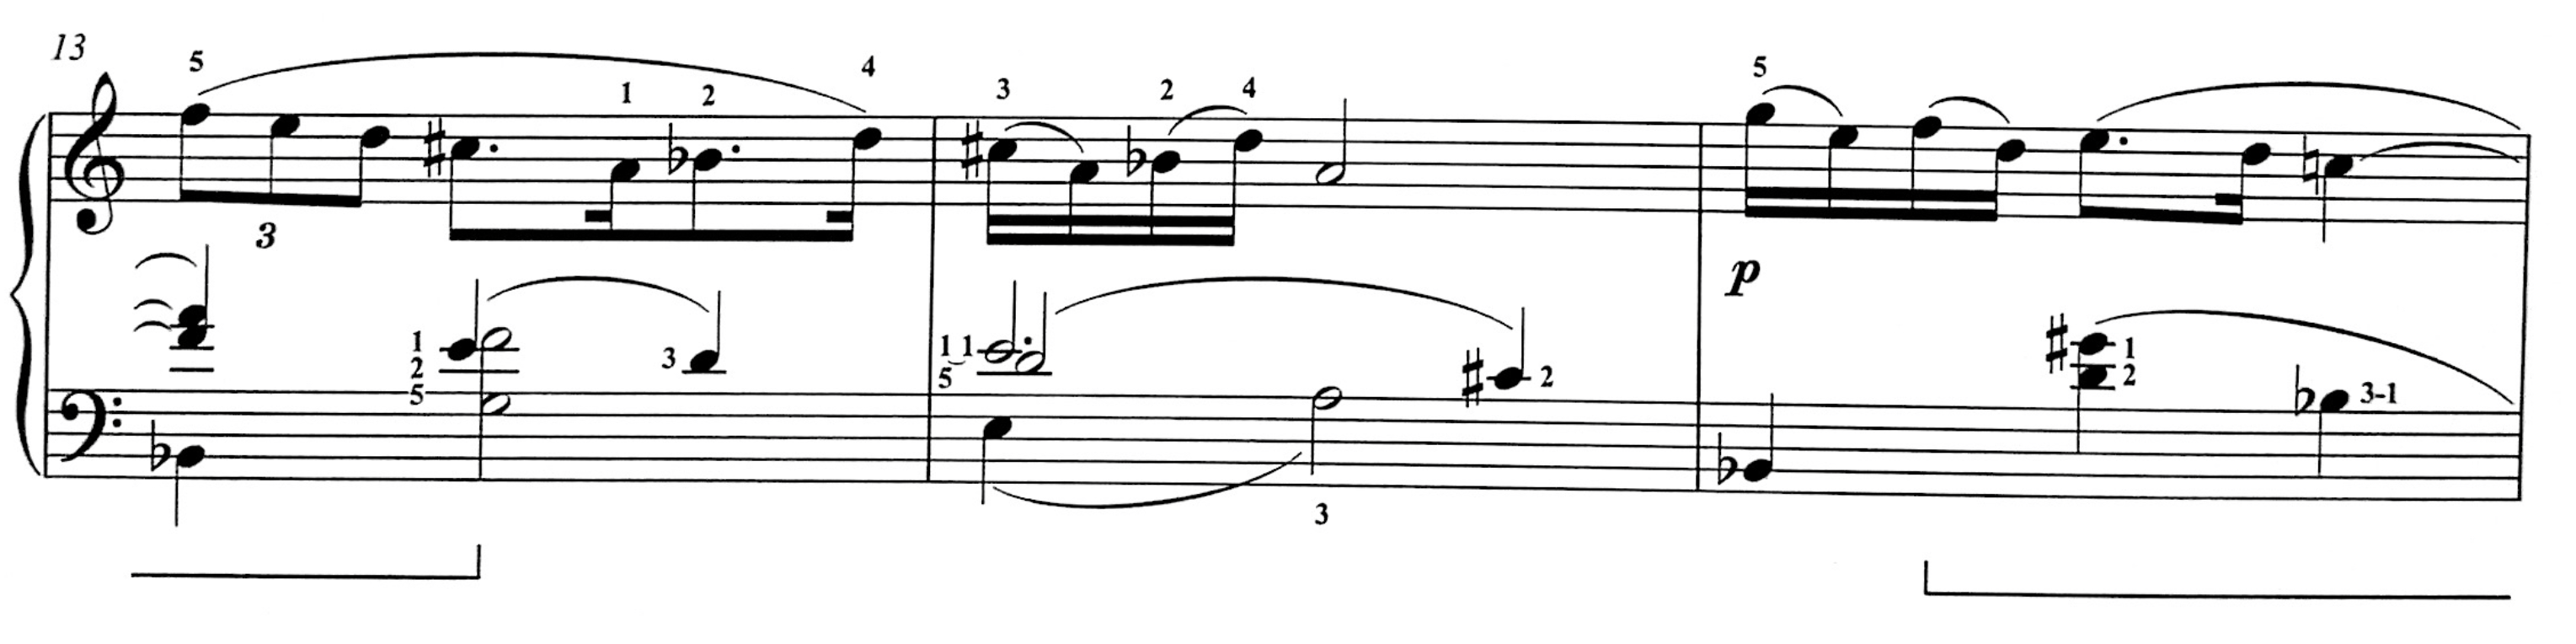
\includegraphics[width=\textwidth]{bartok-dance-four-b-section-second-system.jpg}
  \caption{Béla Bartók, Six Romanian Folk Dances, \textit{Buciumeana},  mm. 13-15}
  \label{fig:legato-notes-example}
\end{figure}

\begin{figure}[h]
  \centering
  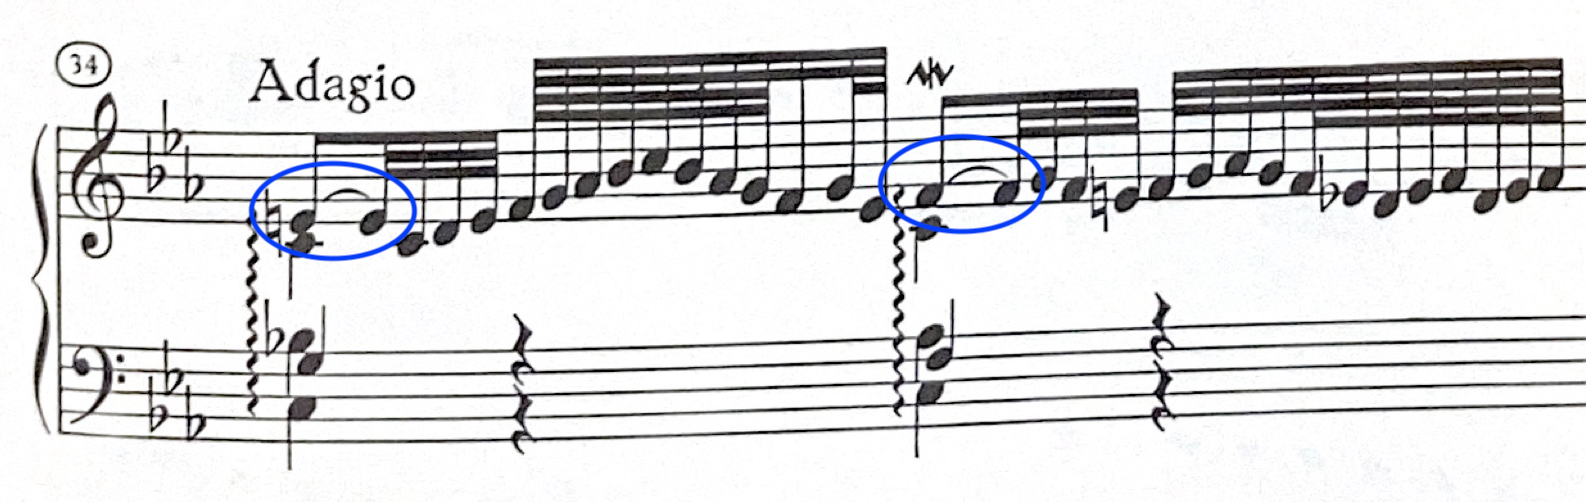
\includegraphics[width=\textwidth]{bach-prelude-second-motive.jpg}
  \caption{Johann Sebastian Bach, The Well-Tempered Clavier Book I, \textit{Prelude in C Minor}, mm. 34-35}
  \label{fig:tied-notes-example}
\end{figure}

\subsection{Major Chord Generator}

The Major Chord Generator within this modular synthesizer involve two pieces: calculating the proper frequencies of the major third and perfect fifth intervals--as they are subject to change from the user's input on the pitch knob--and adding these two intervals to play simultaneously with the original waveform sound. First, to calculate the proper intervals of tonic note to major third, and tonic note to perfect fifth, \textit{interval ratios} (the widths of semitones) are used. As mentioned within Subsection \ref{subsection:how-midi}, the commonly used tuning system in the Western world is the twelve-tone equal temperament system, which divides the octave into 12 parts. Each of these parts are equally tempered (or equally spaced) on a logarithmic scale, such that each ratio is equal to $2^\frac{1}{12}$, or $\sqrt[12]{2} \approx 1.05946$ (the 12th square root of 2, and $a$ in Equation \ref{eq:equal-temperament-eq} \cite{Suits_1998}). This tuning system is normally tuned relative to the standard pitch of 440 Hz, known as \textit{A440}, signifying that the note $A$ (typically $A_4$, or Concert A) is tuned to 440 Hertz, and all other notes are defined relative to this pitch, as some multiple of semitones away from it, either higher or lower in frequency. Thus,  the modular synthesizer created also begins with a starting pitch of A440, every other pitch is defined relative to it ($f_0$ in Equation \ref{eq:equal-temperament-eq}).

Within the twelve-tone equal temperament system, calculating the intervals for the major third and perfect fifth is some multiplication of the single semitone $\sqrt[12]{2}$. As there are four semitones between the tonic note and its major third, the interval ratio is $2^\frac{4}{12}$, or $\sqrt[\frac{4}{12}]{2}$, and seven semitones between the tonic and perfect fifth, the interval ratio is $2^\frac{7}{12}$, or $\sqrt[\frac{7}{12}]{2} \approx \sqrt[12]{128}$, as in Listing \ref{lst:chord-creation} and Equation \ref{eq:equal-temperament-eq}. 

\begin{listing}
	\begin{lstlisting}
		var baseFrequency = 440;
		var thirdFreq = baseFrequency * (2**(4/12));
		var fifthFreq = baseFrequency * (2**(7/12));
	\end{lstlisting}
	\label{lst:chord-creation}
	\caption{Creating the major third and perfect fifth intervals}
\end{listing}

\begin{equation}
	f_n = f_0 * (a)^n
	\label{eq:equal-temperament-eq}
\end{equation}

After calculating the ratio of frequencies, the work on the second part of the module begins. Similar to the work done to create the initial waveform, two additional pure waveforms, and their Synth counterparts, are created (Listing \ref{lst:major-chord-synths}). Then, the only step which remains involves adding the Synths $y$ and $z$ into a variable to play simultaneously (Listing \ref{lst:major-chord-module}) using an array called ``majChord.''

\begin{listing}
	\begin{lstlisting}
		SynthDef("sinewave_third", {arg vol=50; Out.ar(0, SinOsc.ar(thirdFreq, 0, vol))}).add;
		SynthDef("sinewave_fifth", {arg vol=50; Out.ar(0, SinOsc.ar(fifthFreq, 0, vol))}).add;
		y = Synth("sinewave_third");
		z = Synth("sinewave_fifth");
	\end{lstlisting}
	\label{lst:major-chord-synths}
	\caption{Creating SynthDefs for the major third and perfect fifth intervals}	
\end{listing}

\begin{listing}
	\begin{lstlisting}
		majChord = ["sinewave", "sinewave_third", "sinewave_fifth"];
	\end{lstlisting}
	\label{lst:major-chord-module}
	\caption{Combining the three waveform Synths into an array ``majChord''}
\end{listing}

The ``majChord'' variable is placed into a button class \textit{Button}, which has two states, depending on the on/off status of the button itself (Listing \ref{lst:major-chord-button}). Once the button's status is changed to on, all three Synths within the ``majChord'' array will sound at once.

\begin{listing}
	\begin{lstlisting}
		majorChord = Button(awindow, Rect(20, 20, 150, 25)).states_([["Turn Major Chord Off", Color.black, Color.gray], ["Turn Major Chord On", Color.black, Color.yellow]]);	
	\end{lstlisting}
	\label{lst:major-chord-button}
	\caption{Implementing the major chord module using the \textit{Button} class}
\end{listing}

\subsection{Delay Slider}

To create the delay slider, which determines the time which the waveform is delayed, we rely on the same native SuperCollider class we did to create the volume slider: \textit{EZSlider}. Like with the volume slider, we are using the same three arguments: controlSpec, action, and initVal. For the control spec of the delay slider, we must make sure these values match those available in the unit circle, so that the valid range of values is between $\frac{\pi}{6}$ to $\frac{11\pi}{6}$. While it is possible to use values greater than $\frac{11\pi}{6}$, or less than $\frac{\pi}{6}$ in theory, in practice it will sound equivalent to values within this range, as the sine wave will be overlaid directly on top of the possible values in this range. 

\begin{listing}
	\begin{lstlisting}
		delaySlider = EZSlider(awindow, label:"Delay Time", labelHeight:50, labelWidth:100, controlSpec:[(-pi)/6, pi/6], action: {|md| x.set("phase", md.value)}, initVal:0);	
	\end{lstlisting}
	\caption{Creating a delay slider in SuperCollider}
	\label{lst:delay-slider}
\end{listing}

In SuperCollider the time values for delay are calculated in radians, so using the values from the unit circle works well. For the ``action'' argument, similarly to previous modules, the phase of Synth ``x'' is set to be equivalent to the value of the delay slider. The slider itself is initialized to 0, where there is no early or late arrival of the sound.

\subsection{Adding Distortion}

The distortion of a simple pure audio signal involves a SuperCollider class known as \textit{InsideOut}. For this module, both clipping and fuzz are used. As in Listing \ref{lst:distortion-waveforms}, there are two aspects which create the clipping and fuzz effects: a sine wave Unit Generator (UGen), and a \texttt{Pink Noise} UGen. The sine wave UGen allows for the clipping of the sound wave. The \texttt{Pink Noise} UGen is added through the fuzz effect, using the value 30 as the frequency multiplier, and allows us to add a type of colored noise known as ``pink noise.''

\begin{listing}
	\begin{lstlisting}
		// PinkNoise function, with a sine wave UGen at the frequency from pitchKnob
		dist = {InsideOut.ar(SinOsc.ar(baseFrequency) + PinkNoise.ar(0.9, 0), 30, 50)}.scope;
	\end{lstlisting}
	\caption{Creating a distortion module}
	\label{lst:distortion-waveforms}
\end{listing}

Pink noise is used as it is a type of noise which contains all the possible frequencies which a human can hear. Unlike other types of colored noise, pink noise is much less intense. There are multiple types of colored noise, including black, red, blue, brown, and white. However, for music production, the two most popular types of colored noise are white noise and pink noise. White noise operates similarly to white light, encompassing the entire frequency of audible sound from low pitches to high pitches equally. Different frequencies are played randomly across the entire audible range, and normally sounds like radio static \cite{Unison_2021}. When mixing white noise into a pre-existing music mix, white noise fills sonic space similar to how low bass notes fill sonic space in the very low end (refer to Table \ref{tbl:frequency-table-of-human-hearing-general}). Pink noise is very similar to white noise, but constructed differently. It creates equal amplitudes based on the octaves, getting softer and less abrasive-sounding as the pitch rises. Thus, lower frequencies are louder, and higher frequencies are easier to listen to and are softer \cite{Unison_2021}. As it technically has a fundamental frequency, it will sound much more natural than white noise, as natural sounds all have a specific fundamental frequency (defined as the lowest harmonic played).

\section{MIDI Input}\label{section:midi-input}

Input with MIDI in SuperCollider is more complex than creating pure sound waveforms for modular changes; however there are some similarities, we must create three aspects for modular sound synthesis: the \texttt{Synth}, \texttt{SynthDef}, and MIDI functions for MIDI itself to be able to output sound. 

Before any of this, however, the MIDI inputs and the MIDI client must be initialized. As in Listing \ref{lst:initialize-midi}, there are two key steps to using MIDI in SuperCollider: initializing the MIDI client and connecting to the specific MIDI controller that will be used. Once this is done, we can move on to creating the MIDI functionality itself.

\begin{listing}
	\begin{lstlisting}
		MIDIClient.init;
		MIDIIn.connect;
	\end{lstlisting}
	\caption{Initializing the MIDI Client}
	\label{lst:initialize-midi}
\end{listing}

Creating a SynthDef for MIDI input will be the easiest task. To create a SynthDef for MIDI use, we do what is in Listing \ref{lst:midi-synthdef}. 

\begin{listing}
	\begin{lstlisting}
		SynthDef("piano", {arg freq = 440, amp = 0.1, gate = 1;
		var snd, env;
		env = Env.adsr(aLevel, dLevel, sLevel, rTime, amp).kr(2, gate);
		snd = Saw.ar(freq: [freq, freq*1.5], mul: env);
		Out.ar(0, snd)
		}).add;
	\end{lstlisting}
	\caption{Creating a MIDI SynthDef with a ADSR envelope}
	\label{lst:midi-synthdef}	
\end{listing}

Listing \ref{lst:midi-synthdef} describes the necessary aspect in the creation of a SynthDef that will  be compatible with MIDI commands. The ADSR envelope, or ``envelope generator'' (a term which refers to the ``shape'' of a sound, or the contour by which a sound gets louder and softer) is described by its stages: Attack, Decay, Sustain, Release, as in Figure \ref{fig:adsr-envelope} \cite{Puckette_2007}. Some of this was discussed in the Note On and Note Off messages subsections of Section \ref{section:midi-messages}. The order in which sound goes through an envelope generator is important, as sound must travel through the attack, decay, sustain, and release stages in that order, and is unable to go back to any other stage once it comes to a stage. An ADSR envelope generator will first receive a gate input, the variable \texttt{gate}, and raise the value of \texttt{gate} to the maximum volume or voltage (if we were to use a physical envelope generator within an analog synthesizer) the envelope generator is able to output, or the output level that is set over a specific time by the Attack control. The gate is one of the main signal types of a modular synthesizer. It will jump from a base level (normally 0) to a higher one when a new note is meant to start, such as when a user presses down on a MIDI keyboard, or another transition is meant to happen, such as when the next stage of the ADSR envelope is meant to start. When a user presses down on a MIDI keyboard, the gate will typically stay at the level it was given for the duration of that note, and then suddenly drop to its baseline level once the key is released. Thus, when the \texttt{gate} variable is sent through a typical envelope generator like the ADSR envelope generator, the beginning of the gate increases to its maximum volume as it tells the envelope to go through the Attack and Decay stages. As the gate remains at this high level, the envelope may go into the Sustain stage, and then when the gate's volume returns to its baseline level, the envelope will move into the Release stage. 

\begin{figure}
  \centering
  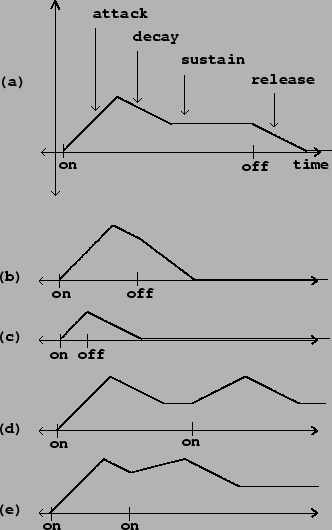
\includegraphics[width=0.4\textwidth]{adsr_envelope.png}
  \caption{ADSR envelope output: (a) with ``on" and ``off" triggers separated; (b) and (c) with early ``off" trigger; (d), (e) re-attacked.} \cite{Puckette_2007}
  \label{fig:adsr-envelope}
\end{figure}

Once the sound reaches this defined high level of the Attack stage, the Decay control will cause the sound to begin dropping in volume, until it reaches the volume set by the Sustain control. If the \texttt{gate} variable is still active (and has a value other than 0), the level set by the Sustain control is maintained until the value of \texttt{gate} returns to 0--which typically signifies the user has released the key on a compatible keyboard or controller. When \texttt{gate} is no longer active, the output volume begins to drop back to a volume of 0, in which the rate of this drop is determined by the Release control. 

A key concept to understanding the ADSR envelope is that there is a difference in behavior when the ADSR envelope is not able to finish the entire four-stage cycle. If the user were to release the key before the Attack or Decay stages finish, then the envelope may skip to the Release stage, passing over the Sustain control entirely, and continuing to the Release control with the current volume level. However, if the user were to re-trigger the envelope by sending a new \texttt{gate} through to the synthesizer, a digital envelope generator will return the volume level back to 0, and restart the envelope cycle.

Other arguments within the SynthDef of Listing \ref{lst:midi-synthdef} include \texttt{freq}, and \texttt{amp}, which will help in modifying the input MIDI key presses. Creating the Synth and MIDI functions for proper MIDI functionality are much more difficult. When creating the waveform modules, there was no need to develop functionality for the waveforms, as they were a native aspect of SuperCollider. Within the MIDI modules, creating the Synth and MIDI functions must be done simultaneously. As in Listing \ref{lst:midi-note-on-and-off}, the two primary MIDI messages that will be used are note on and note off. To create a Synth using the ``piano'' SynthDef from Listing \ref{lst:instantiate-synthedef}, it will be wrapped within the SuperCollider MIDI function for note on: \texttt{MIDIdef.noteOn}. With the proper MIDI functionality created, similar modules to those developed for pure waveforms can be made.

\begin{listing}
	\begin{lstlisting}
		on = MIDIdef.noteOn(\keyDown, {arg vel, note, vol;
				notesArray[note] = Synth("piano", [\freq, note.midicps, \amp, vel.linlin(aLevel, dLevel, sLevel, rTime)]);
			});

		off = MIDIdef.noteOff(\keyUp, {arg vel, note;
				notesArray[note].set(\gate, 0);
			});
	\end{lstlisting}
	\caption{Creating MIDI note on and MIDI note off messages}
	\label{lst:midi-note-on-and-off}	
\end{listing}


\section{The Modules: In Midi}\label{section:the-modules-midi}

Within SuperCollider, the \texttt{Env} class supports the creation of an ADSR envelope, which will allow us to create the modules for the MIDI controller. As in Listing \ref{lst:template-adsr-envelope}  \cite{McCartney_2021}, SuperCollider has native functionality for an ADSR envelope. The first four arguments of the \texttt{ADSR} envelope are consistent as we create the maximum levels for the Attack, Decay, Sustain, and Release stages. The other variable which we are interested in is \texttt{peakLevel}, which in this project is known as \texttt{amp}. This variable is different from \texttt{gate}, as seen in Listing \ref{lst:midi-synthdef}. The \texttt{gate} variable helps determine the current active stage of the ADSR envelope, helping sound move through the envelope one stage at a time. The \texttt{amp} variable on the other hand defines the peak level of each of the stages itself. It is the defining high level of the Attack Stage. Through changing the levels of the Attack, Decay, Sustain, and Release stages, we can modify the input sound from a MIDI controller. 

\begin{listing}
	\begin{lstlisting}
		Env.adsr(attackTime: 0.01, decayTime: 0.3, sustainLevel: 0.5, releaseTime: 1.0, peakLevel: 1.0, curve: -4.0, bias: 0.0)
	\end{lstlisting}	
	\caption{Template for creating an ADSR envelope in SuperCollider}
	\label{lst:template-adsr-envelope}
\end{listing}


\subsection{Volume Slider}

The first module of the MIDI synthesizer, the ``volume'' slider, is a misnomer. While the result is the same, and the output sound from the MIDI controller has a different dynamic level, the logic of the module is different from that of the volume slider within the waveform synthesizer. As mentioned, the \texttt{amp} variable determines the peak level of a MIDI note within an ADSR envelope. Thus, the manipulation of \texttt{amp} is important to adjusting the output volume heard by the user. To then create this amp slider, the SuperCollider class \textit{EZSlider} creates the amp slider, with three arguments: ``controlSpec,'' ``action,'' and ``initVal.'' The control spec for this slider is the same as the volume slider for the waveforms, and cannot be negative, as both negative volume and thus a negative amp value does not exist. Valid values of the control spec is thus between 0.1 and 1, the typical range for an \texttt{amp} value. Then the ``action'' of the slider will determine the volume output of the MIDI input. 

\begin{listing}
	\begin{lstlisting}
		ampSlider = EZSlider(awindow, label:"Amp Volume", labelHeight: 100, labelWidth: 150, controlSpec: ControlSpec(0.1, 1, \lin), action:{|ampSliderValue| note.set(\amp, ampSliderValue.value)}, initVal:0.3);
	\end{lstlisting}	
	\caption{Creating the amp slider for MIDI}
	\label{lst:midi-amp-slider}
\end{listing}

In Listing \ref{lst:midi-amp-slider}, the ``action'' involves altering the input signal from a MIDI controller. The \texttt{note} which holds the information for each note on message is accessed, and the value of the \texttt{note}'s \texttt{amp} is set to be equivalent to the slider's value. The \texttt{amp} value will not continuously update itself, a difference from the volume slider. This difference in functionality is due to the nature of both pure sound waveforms and MIDI signal inputs. Within pure sound waveforms, the signal is continuous, and continues to sound until an external force stops the signal. MIDI signals, on the other hand, rely primarily on the usage of note on and note off messages to send sound to a tool which can properly output it. Thus, the \texttt{amp} of the MIDI note on message of Listing \ref{lst:midi-note-on-and-off} will only update when a new MIDI note on message is sent. Finally, the initial value of the slider is at a \textit{mezzo forte} value of 0.3.

\subsection{Major Chord Generator}

A major chord generator for MIDI will create a major chord, and sound two additional frequencies on top of a MIDI note which a user plays. This will create a triadic chord, with two intervals from the base MIDI note: the major third, and the perfect fifth. The major third interval spans four degrees of the diatonic scale within equal temperament, and the perfect fifth spans seven. As with the major chord generator which was built for pure sound waveforms, the major chord generator for MIDI involves the same two aspects: calculating the proper interval frequencies for the major third and perfect fifth interval, and pushing these two intervals to the SuperCollider server \textit{scsynth}. Using Equation \ref{eq:equal-temperament-eq} and the code from Listing \ref{lst:chord-creation}, we understand that the interval of a major third will have a frequency of $440 * 2^\frac{4}{12}$ and the perfect fifth a frequency of $440 * 2^\frac{7}{12}$.

Thus, having already created the proper intervals for the module, we then must push the intervals to play on \textit{scsynth}. This is different from creating this module for pure waveforms in that we no longer must put the major third and perfect fifth intervals into an array for playback. The SynthDef for MIDI is contained within an ADSR envelope, which has more modularity and independence than pure sound waveforms. Thus, we wrap both the variable for the major third interval (\texttt{thirdInterval}) and the perfect fifth interval (\texttt{fifthInterval}) into variables titled \texttt{thirdIntervalSynth} and \texttt{fifthIntervalSynth} respectively. These variables utilize similar logic to the implementation of \texttt{MIDIdef.noteOn}, layering the intervals on top of the user input.

\begin{listing}
	\begin{lstlisting}
		thirdIntervalSynth = Synth("piano", [\freq, thirdInterval, \amp, vel.linlin(0, 127, 0, 1)]);
		fifthIntervalSynth = Synth("piano", [\freq, fifthInterval, \amp, vel.linlin(0, 127, 0, 1)]);
	\end{lstlisting}
	\label{lst:midi-maj-chord}
	\caption{Creating a major chord in MIDI}
\end{listing}

\subsection{Adding Staccato}

The staccato and legato buttons for the MIDI synthesizer are similar. For this module, we rely heavily on two aspects of the ADSR envelope, the Attack level, and the Decay level. In combination, a shorter attack time and a shorter decay time will create a sudden perceived drop in the volume level of a MIDI input signal. As in Listing \ref{lst:midi-note-on-and-off}, we have created four variables which contain the values for each of the four stages of the ADSR envelope: \texttt{aLevel} for Attack, \texttt{dLevel} for Decay, \texttt{sLevel} for Sustain, and \texttt{rTime} for Release. For this module, the values for \texttt{aLevel} and \texttt{dLevel} are set to 0. With Attack set to 0, the sound of the MIDI input will hit immediately after the signal is begun. Decay set to 0 results in no time for the sound's level to fall from its peak of \texttt{amp} to the \texttt{dLevel}.

\subsection{Adding Legato}

The legato button emulates the musical concept of legato. On a physical MIDI keyboard, a legato button will more often be referenced as a \textit{sustain} button, in which the lengths of notes are extended, and flow into one another. For the concept of legato, it is imperative that each note meant to be played legato are of different pitches. If the pitches of notes meant to be played legato are the same, the duration of these notes will simply be elongated--and the notes tied together--to be the sum of each individual note. Two other aspects of the ADSR envelope are important to extend the sounding of a MIDI note, and to connect it to another MIDI note: Attack and Release. As mentioned, increasing the level of the Attack stage will result in the sound of a MIDI input signal lengthening. This results in more time needing to pass before the gate will move onto the second stage of the ADSR envelope. Extending the time the gate is in the Release stage is also important. For proper legato within MIDI, the Release stage will need to be extended, as the ADSR envelope is only within the note on MIDI message. The note within the MIDI note on message will continue to sound, even after the MIDI note off message is sent through SuperCollider.


\subsection{Distortion}

Distortion, the altering and deforming of an audio signal's waveform, is done to add specific textures and harmonic over what an instrumentalist would play. For this module, we add regular distortion to the input MIDI signal, to add additional harmonics. Regular distortion is the easiest type of distortion to implement for MIDI, as it is similar to how distortion would be added in rock music, and guitar solos, with Jimi Hendrix songs as one example. Distortion in this module will be a kind of gentle distortion in which two pure sound waveforms are added on top of the MIDI signal, when a note on message is sent. 

This module is built differently than the distortion module for pure sound waveforms. With pure sound waveforms, we used simple unit waves--such as sine waves and sawtooth waves--and altered the sound through a native SuperCollider class. The pure sound waves were only ever able to output one frequency at a time, a limitation which does not hold true with MIDI. MIDI can output multiple frequencies at once, through the use of multiple note on messages. So it is much easier to simply add pink noise to a sine wave, at the same frequency as the wave which the user is playing, and run that aggregated sound through a class. With MIDI, though we are also adding additional harmonics over an input MIDI signal, we are not adding colored noise. Instead, as in Listing \ref{lst:midi-distortion}, we borrow some logic from the major chord generator, but use a tritone interval instead of the pleasant-sounding major third and perfect fifth intervals. In place of these two intervals, the tritone interval is used. 

The tritone is the interval of an augmented fourth,\footnote{Enharmonically equivalent to the diminished fifth, both the augmented fourth interval and the diminished fifth interval will sound the same to a listener, but are notated differently.} and in the Medieval era of music was known to be the ``devil in music'' or the ``devil's interval'' because it is the most dissonant interval in the diatonic scale. The diatonic scale is the type of scale which we have discussed, and defined as the scale which contains five whole tones and two semitones \cite{Burkholder_Grout_Palisca_2014}. The major and natural minor scales are diatonic in nature, with the semitones falling between the third and fourth tones in the major scale, and the seventh and eighth tones. In C Major, these semitones would fall between the notes E-F (scale degrees three and four), and notes B-C (scale degrees seven and eight). The minor scale is slightly different, with semitones falling between the second and third scale degrees, and the fifth and sixth degrees. In A Minor, these semitones occur between C-D (degrees three and four), and E-F (degrees five and six).

The tritone is made up of six semitones, and is the interval between C and F\musSharp{}, for example. Its unpleasant sound to the human ear can be traced back to a phenomenon found within the human brain: it is hardwired to find harmony and symmetry within music, and is resistant towards dissonant sounds (rather than pleasing consonant sounds). Intervals which sound pleasing to the human ear are those in which there is a simple ratio between the frequencies. This is clear in the ratios of very pleasant intervals: the octave, which contains the very pleasing 2:1 ratio, and the perfect fifth, which has a ratio of 3:2 \cite{Gann}. These frequency intervals continue through the remaining notes of the scale, oscillating between consonant and dissonant intervals. The tritone, as the most dissonant of all the intervals on the diatonic scale, contains a frequency ratio of 45:32 (or 64:45, depending on the tuning method). 

Distortion for MIDI is not meant to sound as pleasing as adding additional harmonics to an electric guitar signal through an amplifier may be. Instead, for the purposes of this module, the tritone interval is used, to give the distortion an unpleasing effect. The distortion effect is also used for this module, albeit in the simple way of adding two pure sound waveforms over the input MIDI signal. As the tritone interval is six semitones away from a root note, we first calculate the tritone interval to be $f_n = 440 * 2^\frac{6}{12}$, using Concert A as the base frequency. Then, as in Listing \ref{lst:midi-distortion}, the tritone frequency is added to two waveform UGens, \texttt{SinOsc} and \texttt{Saw}, which will add the necessary unpleasant sounds to the MIDI input note's frequency.

\begin{listing}
	\begin{lstlisting}
		tritone = baseFrequency * (2**(6/12));
			
		SynthDef("distortionSynthDef", {arg out = 0;
			Out.ar(out, SinOsc.ar(tritone, 0, 50), Saw.ar(tritone, 0, 50))
		}).add;
	\end{lstlisting}
	\caption{Adding distortion in MIDI}
	\label{lst:midi-distortion}
\end{listing}


\subsection{Manually Adjusting the ADSR Envelope}

The final module for the MIDI synthesizer will be a method of manually adjusting the values for the four pieces of the ADSR envelope. The first five modules of the MIDI synthesizer are ``presets,'' (also known as a ``patch'') or pre-defined modules which are pre-programmed into the synthesizer. These presets, which are also found as all five modules in the pure sound waveform version of the synthesizer, allow a user to understand how an output sound may be changed, without requiring a more in-depth understanding of waveforms or ADSR envelopes. Presets found within a synthesizer are typically modules built to function in a particular way, such that a certain effect can be used to a specified degree. Each synthesizer contains ``parameters'' (like with this modular synthesizer in its ADSR envelope) which allow a user to shape a sound, altering the sound depending on how a user may press, hold, and release keys of a controller. Thus, presets are best understood to be a ``snapshot'' of these parameters (the level of Attack, Decay, Sustain, and Release) at specified values.

The easiest method used to alter the levels of Attack, Decay, Sustain, and Release will be through the SuperCollider class \textit{EZKnob}. This knob class allows for small changes in the value of a variable, and for more flexibility than a simple button may allow. This results in the ability of a user to change the sound of an ADSR envelope to their liking, and can even manually replicate the results of the five other modules, as in Figure \ref{fig:adsr-knobs}. To create the four knobs of Figure \ref{fig:adsr-knobs}, we use the \textit{EZKnob} class four times, once per each knob. Each knob will have the same logic, only affecting different aspects of the ADSR envelope, and with a different initial value to the knob, as in Listing \ref{lst:midi-adsr-manual}. The knob which controls Release will have a larger control spec than the three other stages of the envelope, as we have set the value of Release to be larger within the legato module, to make the legato of MIDI inputs clear.

\begin{figure}[h]
  \centering
  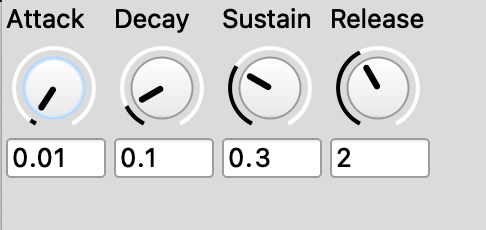
\includegraphics[width=0.4\textwidth]{adsr_knobs.png}
  \caption{The ADSR knobs}
  \label{fig:adsr-knobs}
\end{figure}


\begin{listing}
	\begin{lstlisting}
		attackKnob = EZKnob(awindow, label: "Attack", controlSpec: [0, 1], action:{|attackKnobValue| aLevel = attackKnobValue.value}, initVal: 0.01);

		decayKnob = EZKnob(awindow, label: "Decay", controlSpec: [0, 1], action:{|decayKnobValue| dLevel = decayKnobValue.value}, initVal: 0.1);

		sustainKnob = EZKnob(awindow, label: "Sustain", controlSpec: [0, 1], action:{|sustainKnobValue| sLevel = sustainKnobValue.value}, initVal: 0.3);

		releaseKnob = EZKnob(awindow, label: "Release", controlSpec: [0, 5], action:{|releaseKnobValue| rTime = releaseKnobValue.value}, initVal: 2);
	\end{lstlisting}	
	\caption{Manually adjusting the values of an ADSR envelope}
	\label{lst:midi-adsr-manual}
\end{listing}

As stated, the ability to manually adjust the values for the four stages of the ADSR envelope will allow for greater flexibility, over the pre-programmed values within the other modules of the synthesizer. The combinations of increasing or decreasing the four values will result in different sounds, such that different instruments will appear to have resulted from the alterations. The values for the ADSR envelope which we create in the beginning, in Listing \ref{lst:template-adsr-envelope}, create a sound similar to that of a piano. A piano has a low Attack value, a short Decay time, a relatively medium length but low amp level Sustain, and a short Release time. Other instrument and sound examples, like in Figure \ref{fig:adsr-examples} \cite{Swisher_2019}, are also possible. By setting the Attack and Decay values to be in the middle of the control spec, and Sustain and Release close to 0, a sound similar to that of a kick drum and snare drum is achieved. To create a sound similar to that of a bass guitar or upright bass, set the Decay and Sustain values to be in the middle of the control spec or high, and Attack and Release values to be low. Increasing the level of Attack also will emphasize the initial ``hit'' of the MIDI note on message, causing the sound to appear to be closer. Within music production, this sound would appear to have emphasized the highs and mids (roughly 500 Hz to 4 kHz), and it would become more prominent in a mix. The same is true on the flip side, in which turning down the Attack will make the sound seem to be further away, and give the overall sound more ``space'' and a bigger soundstage. This is best seen in rhythm guitars and bass guitars and upright bass, in which the sound is needed, but should not be a prominent part of a mix. The other method of creating a larger soundstage within the ADSR envelope and a mix is to increase the level of Sustain, as if the microphone used to record the instrument was placed further away. 

\begin{figure}
  \centering
  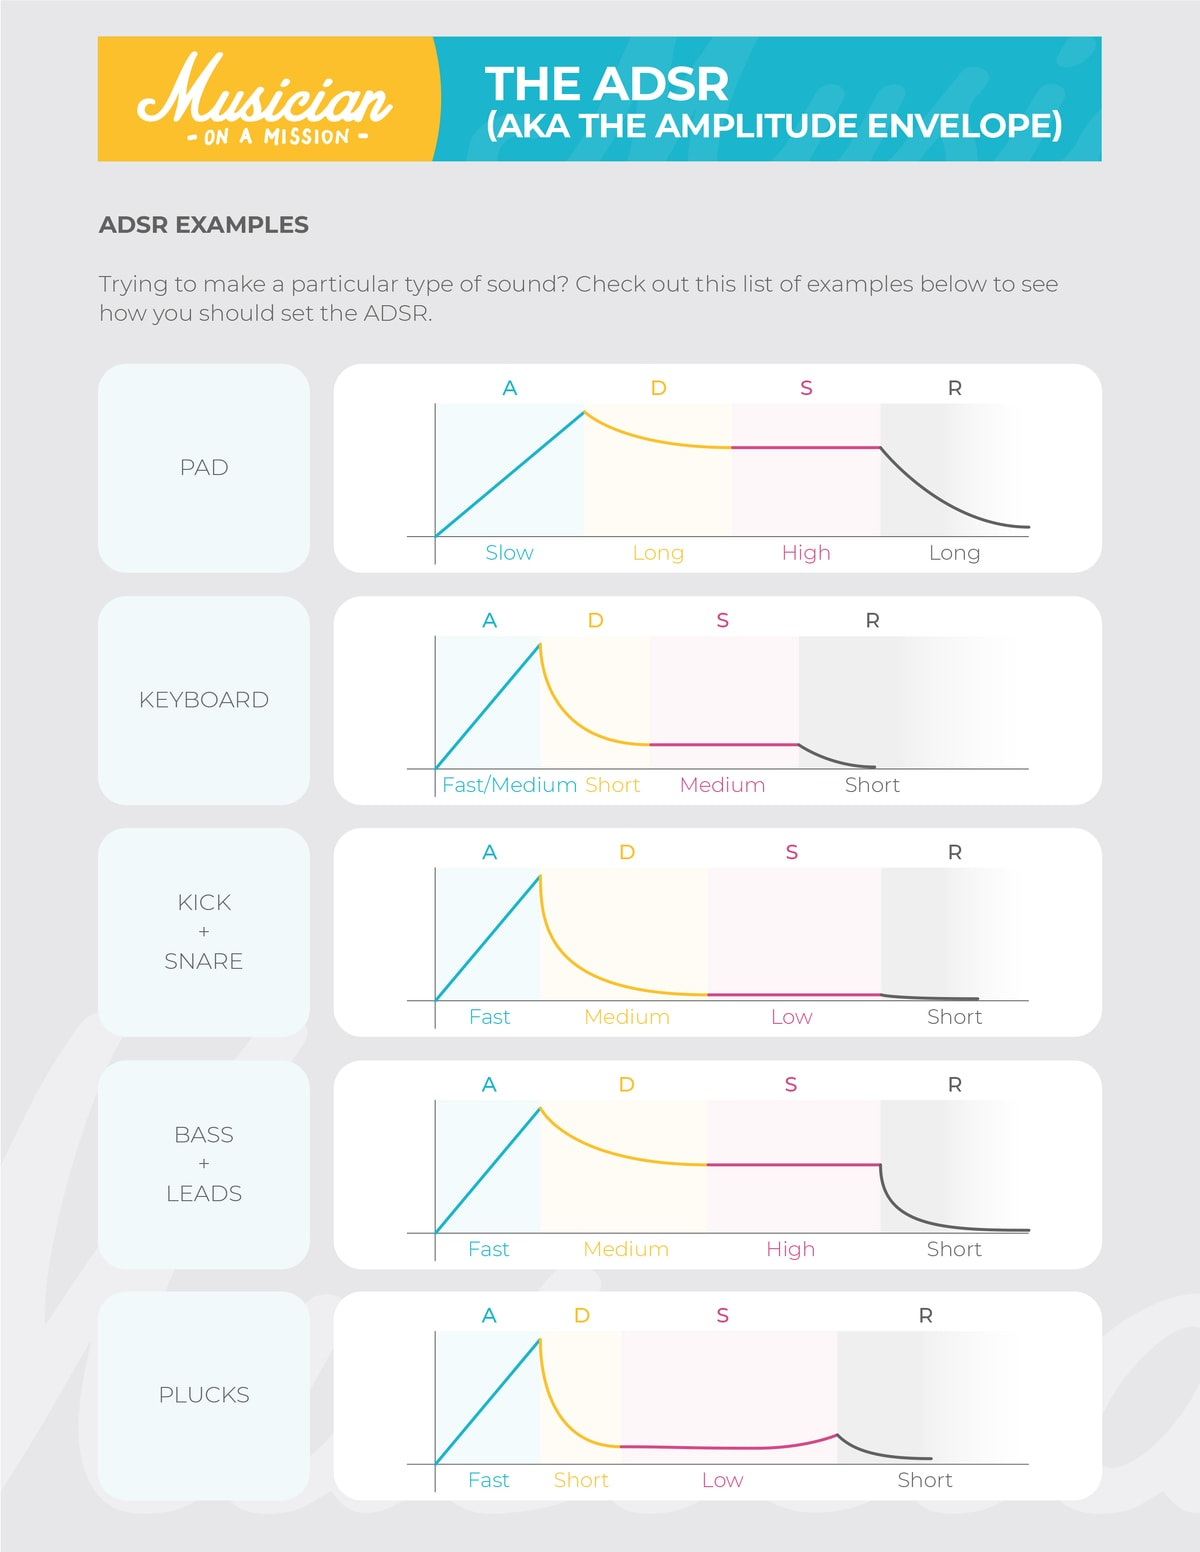
\includegraphics[width=0.4\textwidth]{adsr_examples.jpeg}
  \caption{Other examples of ADSR values} \cite{Swisher_2019}
  \label{fig:adsr-examples}
\end{figure}
\chapter{Conclusion and Future Work}\label{conclusion}

This project resulted in the successful implementation of a modular synthesizer, in which both pure sound waveforms and MIDI signals are used as inputs. Within the timeframe available, we accomplished a set of minimal goals necessary for success. While this thesis project ends with a positive result, there are also multiple ways in which this synthesizer can be improved upon, or extended. To conclude, we review the limitations of implementing this application, the necessary goals of this project, which we accomplished, in addition to the areas in which further research and development can be pursued. 

\section{Challenges}\label{section:limitations}

The development of a virtual modular synthesizer has achieved its goals, but limitations in the process of implementation still exist. The most noticeable in the development of this synthesizer, involves the scope of functions in SuperCollider. SuperCollider has two types of scope for functions and variables: local, and environmental (similar to how many other languages function). If a variable is declared within a certain scope, like a function, the variable will thus have a local value only within that scope, as variable \texttt{a} does in Listing \ref{lst:good-sc-code}. This code lies between parenthetical brackets (simply known as ``brackets'' in SuperCollider) which determine the scope of a variable. However, lowercase letters (a-z, with the exception of `s' which by default is used as a reference to the \textit{scsynth} server) are able to be used with declaration, as are ``environmental'' variables, with contain the \texttt{\~} symbol \cite{McCartney_2016}. While good that some variables are able to be accessed outside a particular scope, this is not good software development. Only single lowercase letters can be global, and if we were to use longer variable names, we would use environmental variables, declared with the \texttt{\~} symbol, and are seen as global variables within SuperCollider. So for the purposes of developing a modular synthesizer, we avoid the usage of global variables to store the necessary information for each module. This requires us to place each module into the same scope, nested into only one set of parenthetical brackets, rather than multiple. We lose the ability to create different functions in different files or classes of code, as the modules must maintain their modularity, or their ability to function in any order, and affect each other.

\section{Completed Goals}

There were several goals that we needed to accomplish in order to build a fully functional modular synthesizer in SuperCollider:

\begin{enumerate}
	\item The application is capable of creating pure sound waveforms and altering these waves.
	\item The application is capable of accepting and altering MIDI input.
	\item The user interface is clean and simple, and makes the interactions the user has with the application easy.
\end{enumerate}

It is clear that the ability of this modular synthesizer to accept and alter either type of input is a minimal requirement of this application, as it is the purpose behind the development of this synthesizer. However, that does not mean that having a clean user interface is a less-important goal. If the functionalities (modules) of this module synthesizer are not implemented with a clean user interface, then the synthesizer may be useless. It necessitates the inclusion of a high-quality and easy-to-use interface, so a user is able to understand each module within this synthesizer, as well as the ways in which each module is meant to alter an output sound. 

\section{Future Work}

The current iteration of this modular synthesizer is easily able to alter input sounds and signals, and output a modification. However, this does not mean that all available features for a modular synthesizer are included in the scope of this project; there are still many ways in which additional features can be added or expanded, including:

\begin{itemize}
	\item Implementing a pitch oscillator for MIDI, which would adjust the frequency of the input signal up or down an octave.
	\item Layering additional sounds and harmonics over both pure sound waveforms and a MIDI input signal, rather than solely harmonics which make up a major chord.
	\item Implementing various fades and filters, to clean up and remove certain frequencies from an output sound.
	\item Adding multichannel support. 
	\item Increasing or decreasing the soundstage of an output sound, determining whether sounds are heard to be very close to the user, or far away.
	\item Adding compression, to ``glue'' sounds together, to make it appear that the sounds belong together, and are not simply layered over one another.
\end{itemize}

Pitch is an important aspect of both music and modular synthesizers. To obtain the correct sound for the instrument of choice, the pitch will need to be altered. For instance, if a user would like to use a bass guitar sound or a bass synth, then the sound will need to be in a lower octave, and the pitch cannot always be Concert A. The ability to layer various sounds over top of each other is an aspect of synthesis which is not fully explored in this project. Layering sounds will allow a user to create a fuller tone and sound, of which the frequencies may or may not be the same. In this synthesizer, we have layered two sounds over a user defined base frequency: a major third interval, and the perfect fifth interval. Additional frequencies which are either the same as the defined base frequency, or within a small difference of the base frequency will result in a bigger sound.

Filters are a fundamental aspect of modular frequencies, especially with the high-pass, low-pass, and band-pass filters. Each of these filter types allow a specific range of frequencies to be removed from the output sound, i.e. high-pass filters allow higher frequencies through, low-pass filters allow lower frequencies, and band-pass filters allow a band, or a certain range, of frequencies. Through the ability to filter out various frequencies, a user's desired sound output can be more easily fulfilled. 

Stereo audio, or multichannel audio, is another aspect of music which is frequently used, but less often within DSP. Creating stereo sound for a modular synthesizer involves increasing the width of the sound. Most noticeable if a user uses headphones while using a synthesizer, stereo audio will feed audio into both the left and right channels, into the left and right ears separately, with slightly different sounds fed into each channel. Thus, sound can be placed as if it were to the left or right of the user, widening the sound output. Adding space to sound output from a modular synthesizer will also allow individual harmonics the room to be heard, and for a user to ``locate'' where the sound is coming from in space. This could also be achieved through the use of heavy reverb and delay effects. Compression would be a useful module to add as well. Using a compressor such as the \textit{bus compressor} would compress every layer of the sound output together into one. This will make the aggregate output sound as if it were one layer, instead of multiple harmonics.

Overall, these features are not essential to create a functioning synthesizer and thus have not yet been implemented. However, these features do add additional benefits and sound modification options to the user, and would be worth implementing in the future. 
%\chapter[Modular Synthesizer]{Building a Virtual Analog Modular Synthesizer}\label{chapter:building-a-mod-synth}

implementation details?
%\input{chapters/chapter5}
%\input{chapters/chapter6}
%\input{chapters/chapter7}
%\chapter{Conclusion and Future Work}\label{conclusion}

This project resulted in the successful implementation of a modular synthesizer, in which both pure sound waveforms and MIDI signals are used as inputs. Within the timeframe available, we accomplished a set of minimal goals necessary for success. While this thesis project ends with a positive result, there are also multiple ways in which this synthesizer can be improved upon, or extended. To conclude, we review the limitations of implementing this application, the necessary goals of this project, which we accomplished, in addition to the areas in which further research and development can be pursued. 

\section{Challenges}\label{section:limitations}

The development of a virtual modular synthesizer has achieved its goals, but limitations in the process of implementation still exist. The most noticeable in the development of this synthesizer, involves the scope of functions in SuperCollider. SuperCollider has two types of scope for functions and variables: local, and environmental (similar to how many other languages function). If a variable is declared within a certain scope, like a function, the variable will thus have a local value only within that scope, as variable \texttt{a} does in Listing \ref{lst:good-sc-code}. This code lies between parenthetical brackets (simply known as ``brackets'' in SuperCollider) which determine the scope of a variable. However, lowercase letters (a-z, with the exception of `s' which by default is used as a reference to the \textit{scsynth} server) are able to be used with declaration, as are ``environmental'' variables, with contain the \texttt{\~} symbol \cite{McCartney_2016}. While good that some variables are able to be accessed outside a particular scope, this is not good software development. Only single lowercase letters can be global, and if we were to use longer variable names, we would use environmental variables, declared with the \texttt{\~} symbol, and are seen as global variables within SuperCollider. So for the purposes of developing a modular synthesizer, we avoid the usage of global variables to store the necessary information for each module. This requires us to place each module into the same scope, nested into only one set of parenthetical brackets, rather than multiple. We lose the ability to create different functions in different files or classes of code, as the modules must maintain their modularity, or their ability to function in any order, and affect each other.

\section{Completed Goals}

There were several goals that we needed to accomplish in order to build a fully functional modular synthesizer in SuperCollider:

\begin{enumerate}
	\item The application is capable of creating pure sound waveforms and altering these waves.
	\item The application is capable of accepting and altering MIDI input.
	\item The user interface is clean and simple, and makes the interactions the user has with the application easy.
\end{enumerate}

It is clear that the ability of this modular synthesizer to accept and alter either type of input is a minimal requirement of this application, as it is the purpose behind the development of this synthesizer. However, that does not mean that having a clean user interface is a less-important goal. If the functionalities (modules) of this module synthesizer are not implemented with a clean user interface, then the synthesizer may be useless. It necessitates the inclusion of a high-quality and easy-to-use interface, so a user is able to understand each module within this synthesizer, as well as the ways in which each module is meant to alter an output sound. 

\section{Future Work}

The current iteration of this modular synthesizer is easily able to alter input sounds and signals, and output a modification. However, this does not mean that all available features for a modular synthesizer are included in the scope of this project; there are still many ways in which additional features can be added or expanded, including:

\begin{itemize}
	\item Implementing a pitch oscillator for MIDI, which would adjust the frequency of the input signal up or down an octave.
	\item Layering additional sounds and harmonics over both pure sound waveforms and a MIDI input signal, rather than solely harmonics which make up a major chord.
	\item Implementing various fades and filters, to clean up and remove certain frequencies from an output sound.
	\item Adding multichannel support. 
	\item Increasing or decreasing the soundstage of an output sound, determining whether sounds are heard to be very close to the user, or far away.
	\item Adding compression, to ``glue'' sounds together, to make it appear that the sounds belong together, and are not simply layered over one another.
\end{itemize}

Pitch is an important aspect of both music and modular synthesizers. To obtain the correct sound for the instrument of choice, the pitch will need to be altered. For instance, if a user would like to use a bass guitar sound or a bass synth, then the sound will need to be in a lower octave, and the pitch cannot always be Concert A. The ability to layer various sounds over top of each other is an aspect of synthesis which is not fully explored in this project. Layering sounds will allow a user to create a fuller tone and sound, of which the frequencies may or may not be the same. In this synthesizer, we have layered two sounds over a user defined base frequency: a major third interval, and the perfect fifth interval. Additional frequencies which are either the same as the defined base frequency, or within a small difference of the base frequency will result in a bigger sound.

Filters are a fundamental aspect of modular frequencies, especially with the high-pass, low-pass, and band-pass filters. Each of these filter types allow a specific range of frequencies to be removed from the output sound, i.e. high-pass filters allow higher frequencies through, low-pass filters allow lower frequencies, and band-pass filters allow a band, or a certain range, of frequencies. Through the ability to filter out various frequencies, a user's desired sound output can be more easily fulfilled. 

Stereo audio, or multichannel audio, is another aspect of music which is frequently used, but less often within DSP. Creating stereo sound for a modular synthesizer involves increasing the width of the sound. Most noticeable if a user uses headphones while using a synthesizer, stereo audio will feed audio into both the left and right channels, into the left and right ears separately, with slightly different sounds fed into each channel. Thus, sound can be placed as if it were to the left or right of the user, widening the sound output. Adding space to sound output from a modular synthesizer will also allow individual harmonics the room to be heard, and for a user to ``locate'' where the sound is coming from in space. This could also be achieved through the use of heavy reverb and delay effects. Compression would be a useful module to add as well. Using a compressor such as the \textit{bus compressor} would compress every layer of the sound output together into one. This will make the aggregate output sound as if it were one layer, instead of multiple harmonics.

Overall, these features are not essential to create a functioning synthesizer and thus have not yet been implemented. However, these features do add additional benefits and sound modification options to the user, and would be worth implementing in the future. 

%%%%%%%%%%%%%%%%%%%%%%%%%%%%%%%%%%%%%%%%%%%%%%%%%%%%%%%
%
%  This section starts the back matter. The back matter includes appendices, indicies, and the
%  bibliography
%
%%%%%%%%%%%%%%%%%%%%%%%%%%%%%%%%%%%%%%%%%%%%%%%%%%%%%%%

\backmatter

\chapter{The Frequency Ranges Within the Human Range of Hearing}\label{appendix:frequency-table}
\begin{table}
	\begin{tabular}{|p{20em}  p{25em}|}
		\hline
		General Frequency Range & Description of Range \\ 
		\hline
		<20Hz - 60Hz & The lowest threshold of human hearing. This includes many frequencies that are felt and not heard, and provides the \say{rumble} feeling in music. This range gives much of music its power, and is typically known as \say{sub-bass}. \\
		\hline
		60Hz - 250Hz & This range determines the amount of \say{warmth} and how full the sound is perceived to be. The notes fundamental to rhythm lives in this range, and too much sound in this frequency range will result in the overall sound being \say{boomy}, or muddy-sounding and messy. It is otherwise known as the the \say{bass} frequency. \\
		\hline
		250Hz - 500Hz & The lower harmonics of many instruments are in this range. It is generally known as the \say{lower midrange} of frequencies, and can introduce listening fatigue and a telephone-quality to the sound if this range is emphasized too much. \\
		\hline
		500Hz - 2 kHz & This range is considered the middle of the midrange. It gives many instruments prominence in a mix, and determines how audible one instrument or vocalist is in comparison to another. If this range is emphasized, audio output may sound tinny and small, which could lead to listening and ear fatigue, as the human ear is sensitive to the human voice, and the frequencies it covers. \\
		\hline
		2 kHz - 4 kHz & The \say{upper midrange} is responsible for much of the attack sounds on percussive and rhythmic instruments. This range may add presence to the mix if boosted, but if it is emphasized too much, it may mask some speech recognition sounds. Listening fatigue may also set in if this range is emphasized too much, as the slightest boost in this range will result in a noticeable change in the sound's timbre. \\
		\hline
		4 kHz - 6 kHz & This range is known as the \say{presence} range. It defines a sound's clarity and the definition of voices and instruments that are present. If this range is boosted, instruments and voices may sound physically closer to the listener, and vice versa, with reducing this range causing instruments and voices to sound further away. However, if this range is emphasized too much, a harsh, irritating sound may occur. \\
		\hline
		6 kHz - 20 kHz & This range controls the \say{brilliance} and clarity of sounds within the mix. Instead of pitches, this range is composed entirely of harmonics, and brings \say{sparkle} to the sound. This range also may easily cause ear fatigue, as an over-emphasis can increase the hiss heard, and produce sibilance, or an unpleasant tonal harnshness which can happen with consonant syllables (most noticeably: S, T, and Z), especially on vocals. \\
		\hline
	\end{tabular}
\caption{The general frequencies ranges, within the range of human hearing}\cite{Suits_1998}\cite{Zjalic_2021}
\label{tbl:frequency-table-of-human-hearing-general}
\end{table}
\chapter{Variables Used}\label{appendix:global-variables}
\begin{table}[h!]
	\begin{tabular}{| c | l |}
		\hline
		Variable & Definition \\
		\hline
		\multirow{2}{*}{f} & temporal frequency (measured in Hertz): \\ & the number of oscillations per unit time \\
		t & time \\
		T & period of a wave \\
		\multirow{2}{*}{$\omega$} & angular frequency: frequency of a sine or \\ & cosine wave as it moves counterclockwise around the unit circle \\
		x & position of a wave along the x-axis \\
		y & displacement of a wave laterally \\
		$y_m$ & amplitude \\
		$\lambda$ & wavelength \\
		\hline
	\end{tabular}
\caption{Variables used in this paper}
\label{tbl:global-variables}
\end{table}
\chapter{Music Theory Terms}\label{appendix:music-theory-terms}
The following list contains the definitions of frequently used musical terms in this paper. Additionally, terms which may augment the understanding of the changes made musically are included. 
\begin{itemize}
    \item {\textbf{Frequency}: the perceived pitch of a sound.}
    \item {\textbf{Volume}: the perceived loudness of a sound.}
    \item {\textbf{Timbre}: the quality of a sound, which helps to differentiate between instruments.}
    \item {\textbf{Staccato}: a directive for notes to be played detached and separated.}
    \item {\textbf{Legato}: a directive for notes to be played smoothly and connected.}
    \item {\textbf{Tie/tied notes}: for this directive, a curved line is drawn over or under the heads of notes of the same pitch. This indicates that there should be no break in the playing of these notes, and should be played as one singular note.}
    \item {\textbf{Chord}: the simultaneous sounding of two or more notes. Typically, a chord will be composed of three notes in total, created a \textit{triad}.}
    \item {\textbf{Major chord}: a chord composed of a root note (the tonic note), a major third interval above the tonic note, and a perfect fifth interval above the tonic note.}
    \item {\textbf{Tonic note}: the note of a chord or a song, which determines the key signature.}
    \item {\textbf{Key signature}: a set of sharp (\musSharp{}, or flat (\musFlat{}) symbols placed on the staff at the beginning of sheet music or a section of music.}
    \item {\textbf{Major third interval}: the interval that spans four semitones. For example, the interval between $C$ and $E$ is a major third.}
    \item {\textbf{Minor third interval}: the interval that spans three semitones. For instance, the interval between $A$ and $C$ is a minor third.}
    \item {\textbf{Texture}: how a sound is organized, and the number of layers within a sound.}
    \item {\textbf{Treble clef}: a type of musical notation to indicate the pitches represented by the lines and spaces on sheet music. Also known as the ``G-clef,'' the second line from the bottom represents the note \textit{G} above Middle C. This clef is the most common clef seen. Typically, the treble clef will contain the note Middle C, as well as notes above Middle C.}
    \item {\textbf{Alto clef}: a type of musical notation to indicate the pitches represented by the lines and spaces on sheet music. This clef is also known as the ``C-clef'' or the ``Viola clef,'' as only certain instruments, which include the viola, use this clef. The middle line of this clef represents the note Middle C.}
    \item {\textbf{Pianissimo}: a directive to perform an indicated passage of a composition or piece very softly. Abbreviated as \textit{pp}.}
    \item {\textbf{Fortissimo}: a directive to perform an indicated passage of a composition or piece very loudly. Abbreviated as \textit{ff}.}
    \item {\textbf{Interval ratio}: the ratios of the frequencies of pitches in a musical interval. As an interval is the ``distance'' between two pitches, the ratio assists musicians to work with relative pitch measures applicable to a range of instruments intuitively, rather than a set of memorized frequency values.}
    
    For instance, suppose we have a guitar as in Figure \ref{fig:guitar-math}. The \textit{interval ratio} will then be inverse to the length of the string. The total length of the string in red has a 1:1 ratio, and the remaining pitches can be described as some ratio to this total string length. On the E string of this guitar (the top string of Figure \ref{fig:guitar-math}), the note an octave above the note E is still E. Then, this note E one octave above the root note E is 12 frets above the root. As noted in the Figure, pressing down on fret 12 of the E string (or any string) results in the length of the string being halved, and an interval ratio of $\frac{1}{2}$. This produces the note one octave above the starting note.
    \item {\textbf{Equal temperament}: a system of tuning the scale, in which the octave is evenly divided into 12 equal semitones. It is based on the cycle of 12 identical fifths, or the ``circle of fifths'' \cite{Cochrane_2011}.}
    
    \begin{figure}[H]
        \centering
        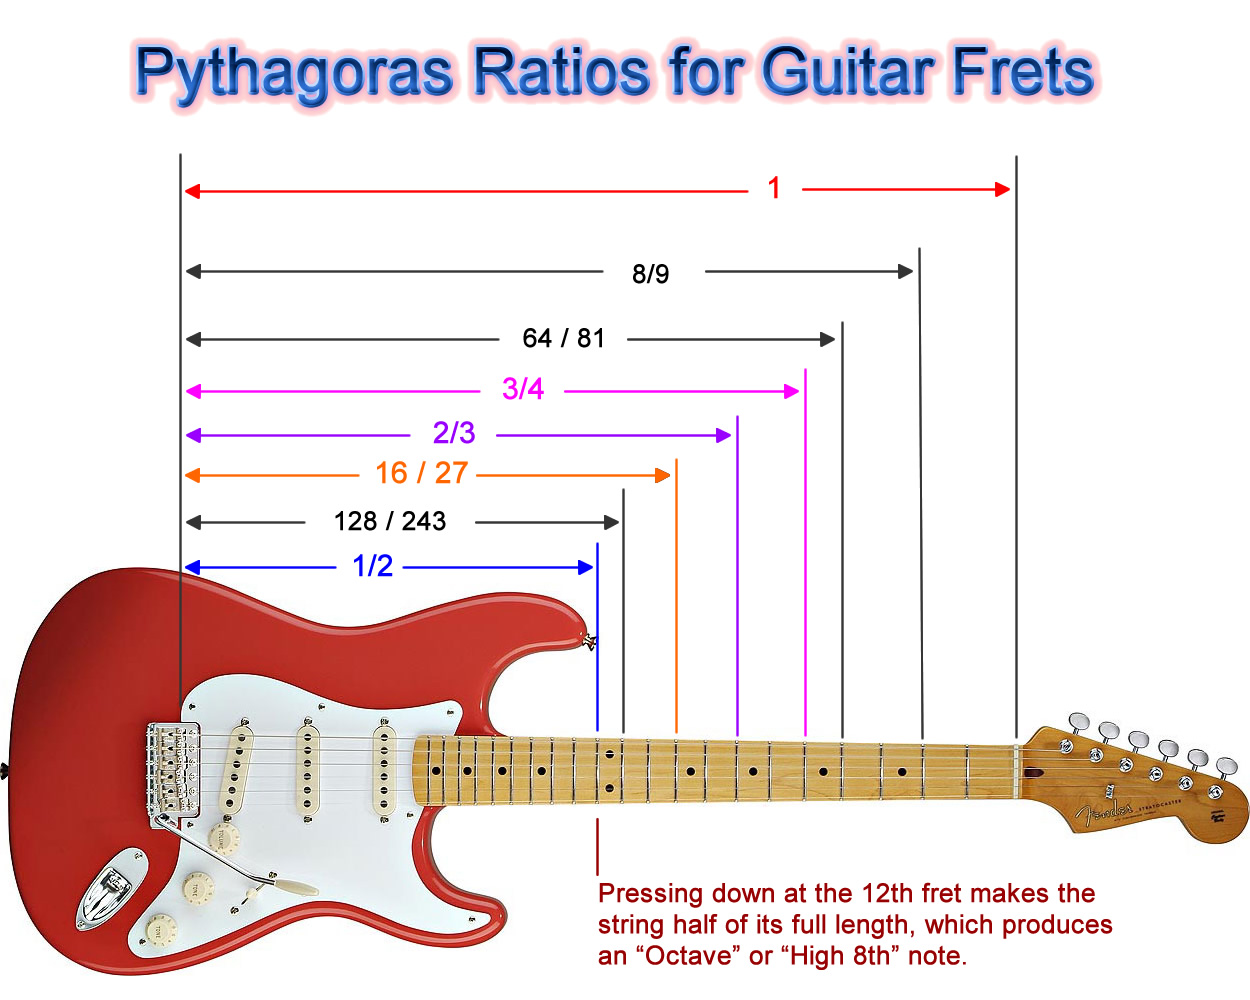
\includegraphics[width=0.4\textwidth]{figures/guitar-math.jpeg}
        \caption{Pythagoras Ratios for Guitar Frets}\cite{Passy_2012}
        \label{fig:guitar-math}
    \end{figure}
    
\end{itemize}
%\input{appendices/java}
%\input{appendices/cpp}
%\input{appendices/afterword}


%%%%%%%%%%%%%%%%%%%%%%%%%%%%%%%%%%%%%%%%%%%%%%%%%%%%%%%
%
%  This section would be used if you are not using BibTeX. Look at Kopka and Daly for how to
%  format a bibliography manually as well as how to use BibTeX.
%
%%%%%%%%%%%%%%%%%%%%%%%%%%%%%%%%%%%%%%%%%%%%%%%%%%%%%%%

%\begin{thebibliography}{99}
%\bibitem{}
%\bibitem{}
%\end{thebibliography}

%%%%%%%%%%%%%%%%%%%%%%%%%%%%%%%%%%%%%%%%%%%%%%%%%%%%%%%
%
%  We used BibTeX to generate a Bibliography. I would recommend this method. However, it is
%  not required.
%
%%%%%%%%%%%%%%%%%%%%%%%%%%%%%%%%%%%%%%%%%%%%%%%%%%%%%%%

\renewcommand\bibname{References} % changes the name of the Bibliography

%\nocite{*} % This command forces all the bibliography references to be printed -- not just 
              % those that were explicitly cited in the text.  If you comment this out, the bibliography
              % will only include cited references.
\bibliographystyle{acm}
% \ifthenelse{\boolean{woosterchicago}}{
% \bibliographystyle{woosterchicago}}{\ifthenelse{\boolean{achemso}}{
% \bibliographystyle{achemso}}{\bibliographystyle{plainnat}}}
% if you have used the woosterchicago class option then your references and citations will be in Chicago format. If you have used the achemso class option then your references and citations will be in the American Chemical Society format. If you do not specify a citation format then the default Wooster format will be used.
\bibliography{references} % load our Bibliography file

%%%%%%%%%%%%%%%%%%%%%%%%%%%%%%%%%%%%%%%%%%%%%%%%%%%%%%%
%
%                                                                Index
%
%  Uncomment the lines below to include an index. To get an index you must put 
%  \index{index text} after any words that you want to appear in the index.
%  Subentries are entered as \index{index text!subentry text}. You must also run the
%  makeindex program to generate the index files that LaTeX uses. The PCs are set to run
%  makeindex automatically.
%
%%%%%%%%%%%%%%%%%%%%%%%%%%%%%%%%%%%%%%%%%%%%%%%%%%%%%%%

%\ifthenelse{\boolean{index}}{
%\cleardoublepage
%\phantomsection
%\addcontentsline{toc}{chapter}{Index}
%\printindex}{}

%%%%%%%%%%%%%%%%%%%%%%%%%%%%%%%%%%%%%%%%%%%%%%%%%%%%%%%
%
%                                                                Colophon
%
%  A Colophon is a section of a printed document that acknowledges the designers and printers of the work.
% The colophon also includes information about the fonts and paper used in the printing. It is not required 
% for your IS and can be commented out.
%
%%%%%%%%%%%%%%%%%%%%%%%%%%%%%%%%%%%%%%%%%%%%%%%%%%%%%%%

%\ifthenelse{\boolean{colophon}}{
%\begin{colophon}
%This Independent Study was designed by Dr. Jon Breitenbucher.\newline
%It was edited and set into type in Wooster, Ohio,\newline
%using the \ifthenelse{\boolean{xetex}}{\XeTeX\ typesetting system designed by Jonathan %Kew}{\LaTeX\ typesetting system designed by Leslie Lamport}\newline
%and based on the original \TeX\ system of Donald Knuth.\newline
%It was printed and bound by Office Services at The College of Wooster.
%
%The text face is Adobe Garamond Pro, designed by Robert Slimbach.\newline
%This is the Opentype version distributed by Adobe Systems\newline
%and purchased as part of the Adobe Type Classics for Learning.
%
%The paper is standard laser copier paper and not of archival quality.
%\end{colophon}}{}
\clearpage\thispagestyle{empty}\null\clearpage
\end{document}